%==============================================================================
% Bakalárska práca — FIT VUT v Brne
% Analýza hashovacích funkcií pre mechanizmus RSS na FPGA sieťovej karte
%
% Postavené na oficiálnej šablóne FIT VUT (2008 Michal Bidlo, 2022 Jaroslav
% Dytrych, 2025 Petr Veigend). Kontakt na správcu šablóny: sablona@fit.vutbr.cz
%
% Kompilácia: pdfLaTeX + BibTeX (v Overleafe stačí Recompile)
% Z konzoly:  make    (viď Makefile)
%==============================================================================
% POZNÁMKY K ÚPRAVÁM OPROTI ORIGINÁLU:
%  - trieda je nastavená na slovenčinu: \documentclass[slovak]{fitthesis}
%  - text práce je rozdelený do súborov kapitoly/*.tex a prilohy/*.tex
%    namiesto pôvodných projekt-01-kapitoly-chapters.tex a
%    projekt-30-prilohy-appendices.tex
%  - pridaný % =====================================================================
%  osnova-makra.tex
%  Makrá na zobrazovanie pokynov v osnove.
%
%  AKO TO FUNGUJE:
%  - kým píšeš, nechaj \osnovatrue  -> pokyny sa vysádzajú sivou farbou
%  - pred odovzdaním daj \osnovafalse -> všetky pokyny zmiznú z PDF,
%    text ostane v zdrojáku (nemusíš nič mazať)
% =====================================================================

\usepackage{xcolor}

\newif\ifosnova
\osnovatrue          % <<< PRED ODOVZDANÍM ZMEŇ NA \osnovafalse

\definecolor{pokyntext}{RGB}{105,105,115}
\definecolor{pokynlinka}{RGB}{180,180,190}
\definecolor{pozorfarba}{RGB}{150,60,60}

% --- základný blok pokynov: \begin{navod}{Nadpis} ... \end{navod} ----
\newenvironment{navod}[1]
  {\ifosnova
     \par\medskip
     \begingroup
     \color{pokyntext}\small\sffamily
     \begin{list}{}{%
       \setlength{\leftmargin}{1.2em}%
       \setlength{\rightmargin}{0.5em}%
       \setlength{\itemindent}{0pt}%
       \setlength{\listparindent}{0pt}%
       \setlength{\parsep}{2pt}%
       \setlength{\topsep}{2pt}}%
     \item[]{\color{pozorfarba}\textbf{#1}}\par\vspace{2pt}%
   \else
     \begingroup\setbox0\vbox\bgroup
   \fi}
  {\ifosnova
     \end{list}\endgroup\par\medskip
   \else
     \egroup\endgroup
   \fi}

% --- jednoriadkové skratky -------------------------------------------
\newcommand{\rozsah}[1]{\ifosnova{\color{pokyntext}\small\sffamily\textbf{Rozsah:} #1\par\medskip}\fi}
\newcommand{\pokyn}[1]{\ifosnova{\color{pokyntext}\small\sffamily #1\par\medskip}\fi}
\newcommand{\pozor}[1]{\ifosnova{\color{pozorfarba}\small\sffamily\textbf{Pozor:} #1\par\medskip}\fi}

% --- TODO priamo v texte (zostane viditeľné aj v „čistom“ režime, aby
%     si ho pri finálnej kontrole nemohol prehliadnuť) ----------------
% Poznámka: titulná strana šablóny sádže niektoré polia verzálkami, čím sa
% \color{todored} zmení na \color{TODORED} — preto je farba definovaná
% v oboch tvaroch. Nemaž ani jednu z nich.
\definecolor{todored}{rgb}{0.80,0.10,0.10}
\definecolor{TODORED}{rgb}{0.80,0.10,0.10}
\DeclareRobustCommand{\TODO}[1]{{\color{todored}\textbf{[TODO: #1]}}}

% --- pomocné makrá používané naprieč prácou ---------------------------
\newcommand{\NDK}{NDK}
\DeclareRobustCommand{\permille}{\textperthousand}
 — makrá na zobrazovanie pokynov v osnove
%    (pred odovzdaním prepni v tom súbore \osnovatrue na \osnovafalse)
%  - anglická vetva (\ifenglish) bola odstránená, práca je po slovensky
%==============================================================================

\documentclass[slovak]{fitthesis}          % bez zadania — pre priebežnú prácu
%\documentclass[slovak,zadani]{fitthesis}  % <<< PRED ODOVZDANÍM: vloží zadani.pdf
%\documentclass[slovak,zadani,print]{fitthesis}  % čiernobiela tlač
%\documentclass[slovak,zadani,cprint]{fitthesis} % farebná tlač, čierne odkazy

% Základné balíčky sú v súbore fitthesis.cls (okrem iného graphicx, amsmath,
% amssymb, booktabs, listings, xcolor, enumitem, todonotes).
% Tu pridávame len to, čo v šablóne nie je:
\usepackage{siunitx}      % jednotky a čísla (\SI, \num) — ak nepoužiješ, zmaž
\usepackage{subcaption}   % podobrázky (\begin{subfigure}) — ak nepoužiješ, zmaž

% Nastavenie cesty k obrázkom / Setting of a path to the pictures
\graphicspath{{obrazky-figures/}{./obrazky-figures/}}

%---rm---------------
\renewcommand{\rmdefault}{lmr}%zavede Latin Modern Roman jako rm
%---sf---------------
\renewcommand{\sfdefault}{qhv}%zavede TeX Gyre Heros jako sf
%---tt------------
\renewcommand{\ttdefault}{lmtt}% zavede Latin Modern tt jako tt

% vypne funkciu šablóny, ktorá automaticky nahrádza úvodzovky
\csdoublequotesoff

\usepackage{url}

% =======================================================================
% balíček "hyperref" musí byť uvedený ako posledný, preto nemôže byť v šablóne
\ifWis
\ifx\pdfoutput\undefined % nejedeme pod pdflatexem
\else
  \usepackage{color}
  \usepackage[unicode,colorlinks,hyperindex,plainpages=false,pdftex]{hyperref}
  \definecolor{hrcolor-ref}{RGB}{223,52,30}
  \definecolor{hrcolor-cite}{HTML}{2F8F00}
  \definecolor{hrcolor-urls}{HTML}{092EAB}
  \hypersetup{
	linkcolor=hrcolor-ref,
	citecolor=hrcolor-cite,
	filecolor=magenta,
	urlcolor=hrcolor-urls
  }
  \def\pdfBorderAttrs{/Border [0 0 0] }
  \pdfcompresslevel=9
\fi
\else % pre tlač budú odkazy čierne
\ifx\pdfoutput\undefined
\else
  \usepackage{color}
  \usepackage[unicode,colorlinks,hyperindex,plainpages=false,pdftex,urlcolor=black,linkcolor=black,citecolor=black]{hyperref}
  \definecolor{links}{rgb}{0,0,0}
  \definecolor{anchors}{rgb}{0,0,0}
  \def\AnchorColor{anchors}
  \def\LinkColor{links}
  \def\pdfBorderAttrs{/Border [0 0 0] }
  \pdfcompresslevel=9
\fi
\fi
% Riešenie problému, keď klikacie odkazy na obrázky vedú za obrázok
\usepackage[all]{hypcap}

% Makrá na pokyny v osnove (pred odovzdaním: \osnovafalse v osnova-makra.tex)
% =====================================================================
%  osnova-makra.tex
%  Makrá na zobrazovanie pokynov v osnove.
%
%  AKO TO FUNGUJE:
%  - kým píšeš, nechaj \osnovatrue  -> pokyny sa vysádzajú sivou farbou
%  - pred odovzdaním daj \osnovafalse -> všetky pokyny zmiznú z PDF,
%    text ostane v zdrojáku (nemusíš nič mazať)
% =====================================================================

\usepackage{xcolor}

\newif\ifosnova
\osnovatrue          % <<< PRED ODOVZDANÍM ZMEŇ NA \osnovafalse

\definecolor{pokyntext}{RGB}{105,105,115}
\definecolor{pokynlinka}{RGB}{180,180,190}
\definecolor{pozorfarba}{RGB}{150,60,60}

% --- základný blok pokynov: \begin{navod}{Nadpis} ... \end{navod} ----
\newenvironment{navod}[1]
  {\ifosnova
     \par\medskip
     \begingroup
     \color{pokyntext}\small\sffamily
     \begin{list}{}{%
       \setlength{\leftmargin}{1.2em}%
       \setlength{\rightmargin}{0.5em}%
       \setlength{\itemindent}{0pt}%
       \setlength{\listparindent}{0pt}%
       \setlength{\parsep}{2pt}%
       \setlength{\topsep}{2pt}}%
     \item[]{\color{pozorfarba}\textbf{#1}}\par\vspace{2pt}%
   \else
     \begingroup\setbox0\vbox\bgroup
   \fi}
  {\ifosnova
     \end{list}\endgroup\par\medskip
   \else
     \egroup\endgroup
   \fi}

% --- jednoriadkové skratky -------------------------------------------
\newcommand{\rozsah}[1]{\ifosnova{\color{pokyntext}\small\sffamily\textbf{Rozsah:} #1\par\medskip}\fi}
\newcommand{\pokyn}[1]{\ifosnova{\color{pokyntext}\small\sffamily #1\par\medskip}\fi}
\newcommand{\pozor}[1]{\ifosnova{\color{pozorfarba}\small\sffamily\textbf{Pozor:} #1\par\medskip}\fi}

% --- TODO priamo v texte (zostane viditeľné aj v „čistom“ režime, aby
%     si ho pri finálnej kontrole nemohol prehliadnuť) ----------------
% Poznámka: titulná strana šablóny sádže niektoré polia verzálkami, čím sa
% \color{todored} zmení na \color{TODORED} — preto je farba definovaná
% v oboch tvaroch. Nemaž ani jednu z nich.
\definecolor{todored}{rgb}{0.80,0.10,0.10}
\definecolor{TODORED}{rgb}{0.80,0.10,0.10}
\DeclareRobustCommand{\TODO}[1]{{\color{todored}\textbf{[TODO: #1]}}}

% --- pomocné makrá používané naprieč prácou ---------------------------
\newcommand{\NDK}{NDK}
\DeclareRobustCommand{\permille}{\textperthousand}



% Informácie o práci / Information about the thesis
%---------------------------------------------------------------------------
\projectinfo{
  %Praca / Thesis
  project={BP},            % typ práce BP/SP/DP/DR
  year={2026},             % rok odovzdania
  date=\today,             % dátum odovzdania
  %Nazov prace / thesis title
  title.cs={Návrh a analýza variantov distribúcie paketov do DMA kanálov jednotkou RSS frameworku NDK},
  title.en={Design and Analysis of Packet Distribution Variants for the RSS Unit of the NDK Framework},
  %title.length={14.5cm},   % odkomentuj, ak sa titulok zle zalamuje
  %sectitle.length={14.5cm},
  %dectitle.length={14.5cm},
  %Autor / Author
  author.name={Marcel},
  author.surname={Kopták},
  %author.title.p={Bc.},
  %author.title.a={},
  %Ustav / Department
  department={UPSY},       % Ústav počítačových systémov — over podľa zadania
  % Školiteľ / supervisor
  supervisor.name={Jiří},
  supervisor.surname={Matoušek},
  supervisor.title.p={Ing.},
  supervisor.title.a={Ph.D.},
  % Školiteľ špecialista (nevypĺňa sa pri BP)
  specialist.name={},
  specialist.surname={},
  specialist.title.p={},
  specialist.title.a={},
  % Klúčové slová / keywords
  keywords.cs={RSS, Receive Side Scaling, DMA kanály, rozloženie záťaže, RETA, Toeplitz, veľké toky, simulácia, FPGA, sieťová karta, NDK, CESNET},
  keywords.en={RSS, Receive Side Scaling, DMA channels, load balancing, RETA, Toeplitz, elephant flows, simulation, FPGA, network interface card, NDK, CESNET},
  % Abstrakt / Abstract
  % ---------------------------------------------------------------------
  % POKYN: abstrakt píš až na konci, 150--200 slov, v tomto poradí:
  %  (1) kontext — vysokorýchlostné FPGA karty a platforma NDK združenia CESNET
  %  (2) problém — nerovnomerná záťaž DMA kanálov pri distribúcii jednotkou RSS
  %  (3) čo si urobil — simulátor do 128 kanálov, metriky, varianty úprav RSS,
  %      analýza nad vzorkami reálnej prevádzky CESNET
  %  (4) hlavný výsledok — hash nerozhoduje, veľké toky áno; orákulum JSQ znižuje
  %      preťaženie o 63--88 %; doplniť výsledok najlepšej varianty
  %  (5) prínos — odporúčanie pre jednotku RSS v NDK
  % ---------------------------------------------------------------------
  abstract.cs={\TODO{abstrakt v slovenčine — štruktúru nájdeš v komentári nad týmto riadkom}},
  abstract.en={\TODO{doslovný preklad slovenského abstraktu; nechaj si ho jazykovo skontrolovať}},
  % Prehlásenie
  % POZOR: šablóna 2025 vyžaduje uviesť použité nástroje umelej inteligencie.
  % Upravte podľa skutočnosti — príklad je nižšie.
  declaration={Prehlasujem, že som túto bakalársku prácu vypracoval samostatne pod vedením pána \TODO{meno vedúceho}.
Ďalšie informácie mi poskytli \TODO{konzultanti, napr. z~CESNETu -- alebo vetu zmažte}.
Uviedol som všetky literárne pramene, publikácie a ďalšie zdroje, z~ktorých som čerpal.
\TODO{Ak ste použili nástroje umelej inteligencie, uveďte ich konkrétne, napr.: Pre jazykovú revíziu technickej správy som použil nástroj X. Pri tvorbe programového kódu som využíval nástroj Y.}},
  % Poďakovanie (nepovinné — ak nechceš, celý riadok zakomentuj)
  acknowledgment={\TODO{Poďakovanie vedúcemu práce, prípadne konzultantom z~CESNETu za poskytnutie datasetov a prístup k~hardvéru. 2--4 vety.}},
  % Rozšírený abstrakt (cca 3 normostrany) — pri BP sa spravidla nevyžaduje
  %extendedabstract={},
  %extabstract.odd={true},
  faculty.cs={Fakulta informačních technologií},
  faculty.en={Faculty of Information Technology},
  department.cs={Ústav počítačových systémů},
  department.en={Department of Computer Systems}
}

% rieši prvý/posledný riadok odseku na predchádzajúcej/nasledujúcej strane
\clubpenalty=10000
\widowpenalty=10000

% checklist
\newlist{checklist}{itemize}{1}
\setlist[checklist]{label=$\square$}

\begin{document}
  % Vysadenie titulných strán / Typesetting of the title pages
  % ----------------------------------------------
  \maketitle
  % Obsah
  % ----------------------------------------------
  \setlength{\parskip}{0pt}

  {\hypersetup{hidelinks}\tableofcontents}

  % Zoznam obrázkov a tabuliek
  \ifczech
    \renewcommand\listfigurename{Seznam obrázků}
  \fi
  \ifslovak
    \renewcommand\listfigurename{Zoznam obrázkov}
  \fi
  {\hypersetup{hidelinks}\listoffigures}

  \ifczech
    \renewcommand\listtablename{Seznam tabulek}
  \fi
  \ifslovak
    \renewcommand\listtablename{Zoznam tabuliek}
  \fi
  {\hypersetup{hidelinks}\listoftables}

  \ifODSAZ
    \setlength{\parskip}{0.5\bigskipamount}
  \else
    \setlength{\parskip}{0pt}
  \fi

  % vynechanie strany v obojstrannom režime
  \iftwoside
    \cleardoublepage
  \fi

  % Text práce / Thesis text
  % ----------------------------------------------
  % !TEX root = ../projekt.tex
% =============================================================================
% STAV: pracovný podklad. Prepísať vlastnými slovami, doplniť citácie.
% =============================================================================
\chapter{Úvod}
\label{chap:uvod}

Rýchlosť počítačových sietí rastie rýchlejšie než výkon jedného jadra procesora.
Pri rýchlostiach 100\,Gb/s a viac už jedno jadro nestíha spracovať všetky prijaté
pakety, preto sieťová karta rozdeľuje prevádzku do viacerých DMA kanálov a každý
kanál obsluhuje iné jadro. \TODO{citácia a konkrétne čísla: čas na jeden paket pri 100\,Gb/s}

Štandardným mechanizmom tohto rozdelenia je \emph{Receive Side Scaling} (RSS).
Z~hlavičky paketu vypočíta hash a podľa neho vyberie DMA kanál. Všetky pakety jedného
toku tak skončia v~tom istom kanáli, čo zachová ich poradie. Cenou za túto vlastnosť je
nerovnomerná záťaž: toky majú veľmi rozdielnu veľkosť a kanál, na ktorý padne niekoľko
veľkých tokov, je preťažený, zatiaľ čo iné kanály majú voľnú kapacitu.

Cieľom práce je navrhnúť a analyzovať varianty distribúcie paketov do DMA kanálov
jednotkou RSS frameworku NDK, vyvíjaného združením CESNET. Práca uvažuje úpravy, ktoré
zachovávajú pravidlo ,,jeden tok = jeden kanál``, aj úpravy, ktoré rozdeľujú pakety
jedného toku na podmnožinu kanálov. Na ich vyhodnotenie vznikol simulátor jednotky RSS
pre najviac 128 DMA kanálov, ktorý pracuje so vzorkami reálnej sieťovej prevádzky.

\TODO{Sem patrí 2--3 vety o hlavnom výsledku, až keď budú hotové varianty z~kapitoly~\ref{chap:vyhodnotenie}.}

\paragraph{Štruktúra práce.}
Kapitola~\ref{chap:ndk} predstavuje platformu NDK. Kapitola~\ref{chap:rss} popisuje
mechanizmus RSS. Kapitola~\ref{chap:metodika} zavádza metriky a metodiku merania
a kapitola~\ref{chap:simulator} implementovaný simulátor. Kapitola~\ref{chap:analyza}
analyzuje východiskové RSS a ukazuje, čo jeho nerovnomernosť spôsobuje.
Kapitola~\ref{chap:varianty} navrhuje varianty úprav, kapitola~\ref{chap:vyhodnotenie}
ich vyhodnocuje a kapitola~\ref{chap:zaver} prácu uzatvára.

  % !TEX root = ../projekt.tex
% =============================================================================
% STAV: iba osnova (bod 1 zadania). Faktami o NDK som kapitolu zámerne neplnil:
% v repozitári k nim nemám zdroje, musia prísť z dokumentácie NDK a od vedúceho.
% =============================================================================
\chapter{Platforma NDK}
\label{chap:ndk}

\TODO{Celá kapitola: čerpať z~dokumentácie NDK a konzultácií s~vedúcim. Odhad 4--6 strán.}

\section{Združenie CESNET a vysokorýchlostné FPGA karty}
\TODO{Čo je CESNET, prečo FPGA, aké karty a rýchlosti sa používajú.}

\section{Architektúra NDK}
\TODO{Bloky firmvéru a cesta paketu od MAC po DMA. Obrázok architektúry.}

\section{DMA kanály}
\TODO{Čo je DMA kanál, koľko ich NDK podporuje, ako sa mapujú na jadrá.
Od vedúceho: pri 100\,Gb/s sa používa približne 8 DMA kanálov. Nájsť citovateľný zdroj.}

\section{Jednotka RSS v~NDK}
\TODO{Kde v~pipeline je, aký hash a kľúč používa, veľkosť RETA, spôsob konfigurácie.
\textbf{Overiť:} simulátor predpokladá Toeplitz, 128 položiek RETA a plnenie $i \bmod n$.}

  % !TEX root = ../projekt.tex
% =============================================================================
% STAV: technický obsah hotový podľa simulátora, chýbajú citácie (bod 2 zadania).
% =============================================================================
\chapter{Mechanizmus RSS}
\label{chap:rss}

RSS rozhoduje o~kanáli každého paketu v~štyroch krokoch:

\begin{enumerate}
  \item z~hlavičky paketu zostaví vstup hashu (\emph{tuple}),
  \item voliteľne ho upraví tak, aby oba smery toku dali rovnaký výsledok (\emph{symetria}),
  \item vypočíta 32-bitový hash s~tajným kľúčom,
  \item spodnými bitmi hashu vyberie položku tabuľky RETA, ktorá určí DMA kanál.
\end{enumerate}

\TODO{Obrázok tejto reťaze. Citácia pôvodnej špecifikácie RSS.}

\section{Vstup hashu}
\label{sec:tuple}

Simulátor používa 36-bajtový vstup. IPv4 adresy sú uložené ako IPv4-mapované IPv6 adresy
(\texttt{::ffff:a.b.c.d}), takže rovnaký formát pokrýva obe verzie IP.

\begin{table}[ht]
  \centering
  \small
  \caption{Rozloženie 36-bajtového vstupu hashu.}
  \label{tab:tuple}
  \begin{tabular}{r l @{\qquad} r l}
    \toprule
    \multicolumn{2}{c}{Plný tuple} & \multicolumn{2}{c}{Iba IP} \\
    Bajty & Pole & Bajty & Pole \\
    \midrule
    0--15  & zdrojová IP   & 0--15  & zdrojová IP \\
    16--17 & zdrojový port & 16--31 & cieľová IP \\
    18--33 & cieľová IP    & 32--35 & nuly \\
    34--35 & cieľový port  &        & \\
    \bottomrule
  \end{tabular}
\end{table}

Protokol do hashu nevstupuje. Porty sú zapísané v~sieťovom poradí bajtov.

\section{Symetria}
\label{sec:symetria}

Bez symetrie majú dva smery toho istého spojenia rôzny tuple a môžu skončiť v~rôznych
kanáloch. Aplikácie, ktoré spracúvajú celé spojenie, však potrebujú oba smery spolu.
Simulátor porovnáva tri režimy:

\begin{description}
  \item[none] tuple sa nemení,
  \item[xor] obe polovice sa nahradia hodnotou $\mathit{src} \oplus \mathit{dst}$,
  \item[sort] väčšia polovica (porovnanie po bajtoch) ide vždy prvá.
\end{description}

Hranica polovíc je na offsete 18 pri plnom tuple a 16 pri variante iba s~IP.

\section{Hashovacie funkcie}
\label{sec:hashe}

Referenčnou funkciou je Toeplitzov hash, štandard pre RSS. Porovnávali sa s~ním
jhash (lookup3), Chaskey, HalfSipHash a jednoduchá tabelácia (\emph{simple tabulation}).
Simulátor má navyše obálky pre multiply-shift (NH), SipHash a XOR hash.
Každá funkcia sa hodnotí so 16 náhodnými 40-bajtovými kľúčmi s~pevným semienkom.

\TODO{Ku každej funkcii 1 odsek: princíp, citácia, náročnosť v~HW. Skrátiť oproti pôvodnému
zadaniu, hash už nie je hlavná téma.}

\section{Tabuľka RETA}
\label{sec:reta}

RETA (\emph{redirection table}) je tabuľka, ktorá prevádza hash na kanál. Spodných
7 bitov hashu vyberie jednu zo 128 položiek. Položka~$i$ je predvolene nastavená na kanál
\begin{equation}
  \mathit{kanal}(i) = i \bmod n .
\end{equation}

\paragraph{Kvantizácia RETA.}
Ak $n$ nedelí 128, položky sa nedajú rozdeliť rovnomerne. Pri $n=20$ má 8 kanálov po
7 položkách a 12 kanálov po 6. Pri $n=40$ má 8 kanálov po 4 položkách a 32 kanálov po 3.
Aj dokonalý hash preto dáva nenulové preťaženie (definícia v~sekcii~\ref{sec:metriky}):
\begin{align}
  n=20: &\quad 8 \cdot \left(\tfrac{7}{128} - \tfrac{1}{20}\right) \cdot 1000 = 37{,}5\,\text{\textperthousand}, \\
  n=40: &\quad 8 \cdot \left(\tfrac{4}{128} - \tfrac{1}{40}\right) \cdot 1000 = 50{,}0\,\text{\textperthousand}.
\end{align}
Namerané hodnoty pri váhe \texttt{flow} sú 38,2 a 51,3\,\textperthousand, teda takmer celé
preťaženie pri týchto počtoch kanálov spôsobuje tabuľka, nie hash.

\section{Hlavné obmedzenie RSS}

RSS rozhoduje iba podľa hlavičky. Nevie, aký veľký tok je ani ako sú kanály práve
zaťažené. Keďže celý tok ide do jedného kanála, jeden veľký tok (\emph{elephant flow})
môže kanál preťažiť bez ohľadu na kvalitu hashu. Túto hypotézu overuje
kapitola~\ref{chap:analyza}.

  % !TEX root = ../projekt.tex
% =============================================================================
% STAV: hotové podľa kódu, doplniť citácie metrík (bod 3 zadania, 1. časť).
% =============================================================================
\chapter{Metriky a metodika merania}
\label{chap:metodika}

\section{Dáta}
\label{sec:data}

Vstupom sú záznamy tokov zo siete CESNET v~CSV s~11 stĺpcami: začiatok a koniec toku,
zdrojová a cieľová IP adresa a port, protokol a počty bajtov a paketov v~oboch smeroch.
Hlavným vzorkom je \texttt{odid1}: približne 35 miliónov záznamov, ktoré po rozvinutí
dávajú približne 2,28 miliardy paketov a súčasne až približne 782 tisíc živých smerov tokov.

\TODO{Doplniť: odkiaľ dáta sú, kedy a na akej linke boli zachytené, priemerná rýchlosť v~Gb/s.}

\paragraph{Známe vlastnosti dát.}
\begin{itemize}
  \item \textbf{Zrkadlené duplicity.} \texttt{odid1} obsahuje zrkadlené záznamy tokov
        (približne 12\,\% riadkov a 42\,\% paketov). Na výreze dát nadhodnocovali preťaženie
        o~2--4\,\%, poradie funkcií nemenili. Výsledky v~tejto práci sú zatiaľ
        \textbf{s~duplicitami}. \TODO{Rozhodnúť: finálne čísla na \texttt{odid1\_dedup}, alebo to uviesť ako obmedzenie.}
  \item \textbf{Okrajový efekt.} Na začiatku záznamu chýbajú už bežiace toky a na konci
        zostávajú iba dlhé toky. Pri Toeplitze, váhe \texttt{packet} a 32 kanáloch je priemerné
        preťaženie v~prvých 10\,\% okien 138,1\,\textperthousand, v~stredných 80\,\% 90,2
        a v~posledných 10\,\% 137,1\,\textperthousand.
\end{itemize}

\section{Rekonštrukcia prúdu paketov}
\label{sec:rekonstrukcia}

Dáta popisujú toky, RSS však pracuje s~paketmi. Každý smer toku sa preto rozvinie na pakety
rozložené rovnomerne medzi začiatkom a koncom toku. Paket $k$ z~$N$ má čas
\begin{equation}
  t_k = t_\mathit{start} + (t_\mathit{end} - t_\mathit{start}) \cdot \frac{k}{N-1} .
\end{equation}
Pakety všetkých tokov sa spájajú podľa času pomocou minimovej haldy. Halda obsahuje iba
živé toky, preto pamäť nerastie s~počtom paketov.

\emph{Obmedzenie:} skutočné pakety rovnomerne rozložené nie sú, zhluky v~rámci toku
simulácia nevidí.

\section{Váha paketu}
\label{sec:vahy}

\begin{description}
  \item[flow] každý smer toku je jedna jednotka; meria kvalitu hashu bez vplyvu veľkosti toku,
  \item[packet] každý paket má váhu 1,
  \item[byte] paket váži priemernú veľkosť paketu svojho toku.
\end{description}

\section{Metriky}
\label{sec:metriky}

Nech $x_i$ je záťaž kanála~$i$ v~okne, $n$ počet kanálov a $W=\sum_i x_i$ celková záťaž okna.

\paragraph{Preťaženie} je podiel záťaže nad spravodlivým podielom, v~promile:
\begin{equation}
  O = \frac{\sum_{i} \max\left(0,\, x_i - W/n\right)}{W/1000} .
\end{equation}
Hodnota 0 znamená dokonale rovnomerné rozdelenie. Prakticky je to podiel prevádzky, ktorý by
bolo treba presunúť z~preťažených kanálov, aby boli všetky rovnako zaťažené.

\paragraph{Jainov index férovosti}~\TODO{citácia}
\begin{equation}
  J = \frac{\left(\sum_i x_i\right)^2}{n \sum_i x_i^2} , \qquad J \in \left[\tfrac{1}{n}, 1\right].
\end{equation}

\paragraph{Normalizované $\chi^2$}, kde $e = W/n$:
\begin{equation}
  \chi^2_\mathit{norm} = \frac{1}{W} \sum_i \frac{(x_i - e)^2}{e} .
\end{equation}

\section{Okná merania}
\label{sec:okna}

Záťaž sa vyhodnocuje v~nezávislých oknách s~pevným počtom paketov. Po každom okne sa
počítadlá vynulujú a neúplné posledné okno sa zahodí. Výsledok jednej konfigurácie je priemer
cez okná a cez 16 kľúčov. Okná sa porovnávali v~dvoch režimoch:

\begin{description}
  \item[pevné okno] 150\,000 paketov pre každý počet kanálov,
  \item[dynamické okno] 18\,750 paketov na kanál, teda $18\,750 \cdot n$ paketov
        (150\,000 pri 8 kanáloch, 2\,400\,000 pri 128).
\end{description}

Dôvod dynamického okna: pri pevnom okne pripadá pri 128 kanáloch na kanál iba približne
1\,170 paketov. Dynamické okno drží rovnaký počet paketov na kanál.

\paragraph{Zvažované a zamietnuté: výber časti tokov.}
Väčšia linka nesie viac prevádzky, preto sme skúšali simulovať menší počet kanálov na
pomernej časti tokov (8 kanálov = 1/16 tokov). Zamietli sme to, lebo by sa pri malom počte
kanálov nepoužila väčšina dát a výsledok by závisel od toho, ktoré veľké toky sa do výberu
dostanú.

\emph{Obmedzenie dynamického okna:} všetky počty kanálov vidia rovnakú prevádzku, takže
pri 128 kanáloch trvá okno 16-krát dlhšie a na kanál pripadá menej tokov.
\TODO{Overiť na datasete s~vyššou prevádzkou, ak ho vedúci poskytne.}

  % !TEX root = ../projekt.tex
% =============================================================================
% STAV: hotové podľa aktuálneho kódu (bod 3 zadania, 2. časť).
% =============================================================================
\chapter{Simulátor jednotky RSS}
\label{chap:simulator}

Simulátor \texttt{rss\_sim} je napísaný v~C++17. Na zachytenej prevádzke simuluje
jednotku RSS s~najviac 128 DMA kanálmi a pre každé okno vyhodnotí záťaž kanálov.
Zámerne oddeľuje \emph{rozhodovanie} (RSS) od \emph{merania}, aby nová varianta RSS
nemohla ovplyvniť spôsob merania.

\section{Architektúra}

\begin{table}[ht]
  \centering
  \small
  \caption{Hlavné časti simulátora.}
  \label{tab:subory}
  \begin{tabular}{l p{9.5cm}}
    \toprule
    Súbor & Úloha \\
    \midrule
    \texttt{settings}    & načítanie konfiguračného súboru \\
    \texttt{parser}      & prevod riadku CSV na tuple a počty paketov \\
    \texttt{flow\_expand} & rekonštrukcia prúdu paketov v~čase (halda) \\
    \texttt{rss}         & reťaz RSS: symetria, hash, RETA alebo modulo, orákulum JSQ \\
    \texttt{simulation}  & rozhodnutia tokov, počítanie paketov, okná, zápis výsledkov \\
    \texttt{metrics}     & preťaženie, Jainov index, $\chi^2$ \\
    \texttt{wrappers/}   & jednotné rozhranie ôsmich hashovacích funkcií \\
    \texttt{analyze.py}  & súhrnná tabuľka a graf \\
    \bottomrule
  \end{tabular}
\end{table}

Beh sa nastavuje jediným súborom:

\begin{lstlisting}
data      = data/odid1.csv
out       = results/result.csv
hash      = toeplitz        # jhash chaskey halfsiphash simpletab ...
tuple     = full            # ip
symmetry  = none            # xor sort
reta      = on              # off
scaling   = on              # off = fixed window
weighting = packet          # flow byte
keys      = 16
channels  = 8 16 20 32 40 64 128
window    = 150000          # used when scaling = off
can_size  = 18750           # packets per channel, scaling = on
\end{lstlisting}

\section{Priebeh simulácie}

Generátor prúdu paketov volá simulátor v~troch momentoch:

\begin{enumerate}
  \item \textbf{Začiatok toku.} Simulátor pridelí toku pamäťový slot. Reťaz RSS vypočíta
        kanál pre každý kľúč a počet kanálov (16~$\times$~7 = 112 hodnôt) a orákulum JSQ
        vyberie svoj kanál.
  \item \textbf{Paket.} Simulátor iba prečíta uložené kanály a pripočíta váhu paketu do
        histogramov. Hash sa pri pakete nepočíta. Keď sa okno daného počtu kanálov naplní,
        vypočítajú sa metriky, zapíše sa riadok výsledkov a vynulujú sa počítadlá tohto
        počtu kanálov.
  \item \textbf{Koniec toku.} Slot sa uvoľní pre ďalší tok, takže pamäť závisí od počtu
        súčasne živých tokov, nie od ich celkového počtu.
\end{enumerate}

\section{Orákulum JSQ}
\label{sec:jsq}

Orákulum \emph{Join the Shortest Queue} (JSQ) slúži ako \textbf{dolná hranica}: ukazuje, čo
sa dá dosiahnuť pri zachovaní pravidla ,,jeden tok = jeden kanál``, ak by jednotka poznala
veľkosť a trvanie toku už pri jeho začiatku. V~hardvéri sa takto realizovať nedá.

Nový tok ide do kanála s~najmenšou očakávanou záťažou na konci aktuálneho okna:
\begin{equation}
  \mathit{ch} = \arg\min_{i} \left( h_i + t_\mathit{left} \cdot r_i \right) ,
\end{equation}
kde $h_i$ je záťaž doručená v~tomto okne, $r_i$ súčet rýchlostí živých tokov na kanáli a
$t_\mathit{left}$ odhad času do konca okna (chýbajúce pakety delené rýchlosťou všetkých živých
tokov). Toky kratšie než 1\,ms sa do rýchlostí nezapočítavajú.

Skúšali sme štyri verzie (syntetické dáta, váha \texttt{packet}, porovnanie s~Toeplitzom):

\begin{description}
  \item[A] kumulatívna záťaž od začiatku: horšie než hash o~4--10\,\%,
  \item[B] záťaž aktuálneho okna: $-19$\,\% pri 8 kanáloch, $+1$\,\% pri 128,
  \item[C] najmenej aktívnych tokov: približne ako hash,
  \item[D] doručená záťaž a očakávaný zvyšok (vzorec vyššie): $-23$\,\% pri 8 kanáloch,
        $-5$\,\% pri 128. Túto verziu sme ponechali.
\end{description}

\section{Overenie správnosti}

Pri prepise simulátora sa výsledky porovnávali s~pôvodnou implementáciou:

\begin{itemize}
  \item na malom testovacom datasete všetkých 180 kombinácií (5 hashov, 2 tuple,
        3 symetrie, RETA zap./vyp., 3 váhy), spolu 108\,360 riadkov,
  \item na celom \texttt{odid1} 212\,660 riadkov (15\,190 okien, 7 počtov kanálov, Toeplitz a JSQ).
\end{itemize}

Najväčší relatívny rozdiel bol menší než $10^{-5}$ a pochádza zo zaokrúhlenia uložených
hodnôt pri priemerovaní cez kľúče. Hodnoty JSQ na \texttt{odid1} sa zhodovali presne.

\TODO{Doplniť čas behu a spotrebu pamäte na \texttt{odid1}.}

  % !TEX root = ../projekt.tex
% =============================================================================
% STAV: výsledky na odid1 sú hotové. Chýbajú ďalšie vzorky (bod 5 zadania).
% Všetky čísla pochádzajú zo super_results/ (pevné okno) a results/baseline.csv
% (dynamické okno, Toeplitz, packet, bez symetrie).
% =============================================================================
\chapter{Analýza východiskového RSS}
\label{chap:analyza}

Táto kapitola odpovedá na otázku, \emph{čo spôsobuje nerovnomernú záťaž kanálov}. Od odpovede
závisí, ktoré úpravy z~kapitoly~\ref{chap:varianty} majú zmysel.

Ak nie je uvedené inak, výsledky sú z~\texttt{odid1} s~plným tuple, RETA so 128 položkami,
16 kľúčmi a pevným oknom 150\,000 paketov (15\,190 okien pri váhach \texttt{packet}
a \texttt{byte}, 287 pri \texttt{flow}).

\section{Príčinou sú veľké toky}
\label{sec:slony}

% !TEX root = ../projekt.tex
\begin{table}[ht]
  \centering
  \small
  \caption{Toeplitz bez symetrie, pevné okno 150\,000 paketov, \texttt{odid1}: priemer cez 16 kľúčov a všetky okná.}
  \label{tab:toeplitz-vahy}
  \begin{tabular}{r rr rr rr}
    \toprule
    & \multicolumn{2}{c}{flow} & \multicolumn{2}{c}{packet} & \multicolumn{2}{c}{byte} \\
    Kanály & [\textperthousand] & Jain & [\textperthousand] & Jain & [\textperthousand] & Jain \\
    \midrule
    8 & 5,5 & 1,000 & 52,3 & 0,981 & 72,0 & 0,965 \\
    16 & 7,6 & 0,999 & 73,3 & 0,962 & 101,0 & 0,932 \\
    20 & 38,2 & 0,993 & 86,3 & 0,950 & 116,3 & 0,912 \\
    32 & 10,4 & 0,999 & 99,6 & 0,929 & 139,4 & 0,873 \\
    40 & 51,3 & 0,983 & 122,4 & 0,900 & 162,2 & 0,836 \\
    64 & 14,0 & 0,998 & 134,4 & 0,870 & 187,4 & 0,779 \\
    128 & 19,0 & 0,995 & 176,5 & 0,774 & 243,2 & 0,645 \\
    \bottomrule
  \end{tabular}
\end{table}


Tabuľka~\ref{tab:toeplitz-vahy} ukazuje ten istý hash pri troch spôsoboch počítania záťaže.
Keď má každý tok rovnakú váhu, je rozdelenie takmer dokonalé: pri 128 kanáloch je preťaženie
19,0\,\textperthousand{} a Jainov index 0,995. Keď sa započíta skutočný počet paketov alebo
bajtov, preťaženie stúpne na 176,5, resp. 243,2\,\textperthousand{} a Jainov index klesne na
0,774, resp. 0,645.

Hash teda rozdeľuje \emph{toky} rovnomerne. Nerovnomerná je \emph{prevádzka}, lebo toky majú
veľmi rozdielnu veľkosť. Preťaženie navyše rastie s~počtom kanálov: čím menší je spravodlivý
podiel jedného kanála, tým väčšiu časť z~neho zaberie jeden veľký tok.

\begin{figure}[ht]
  \centering
  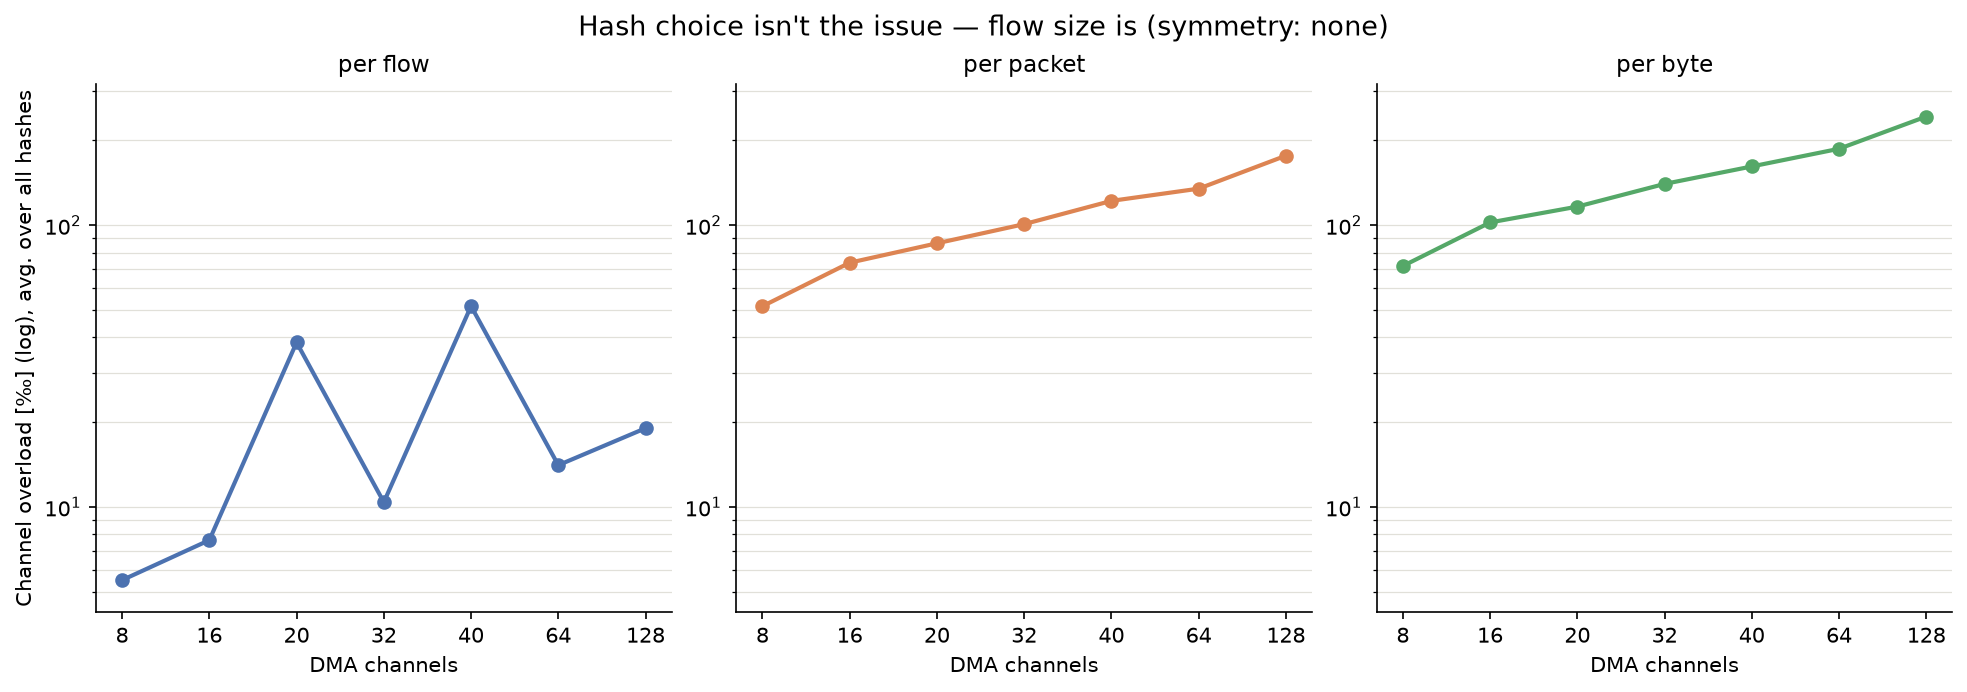
\includegraphics[width=\textwidth]{analyza/elephant_evidence.png}
  \caption{Preťaženie spriemerované cez všetky hashe pri troch váhach (logaritmická os).
  Špičky pri 20 a 40 kanáloch vo váhe flow spôsobuje kvantizácia RETA.
  \TODO{Prekresliť so slovenskými popismi.}}
  \label{fig:slony}
\end{figure}

\section{Porovnanie hashovacích funkcií}
\label{sec:hash-nezalezi}

Porovnávalo sa päť funkcií: Toeplitz, jhash, Chaskey, HalfSipHash a jednoduchá tabelácia.
Každá so 16 kľúčmi, tromi režimami symetrie, tromi váhami a siedmimi počtami kanálov, teda
5\,040 kombinácií na vzorke \texttt{odid1}.

% !TEX root = ../projekt.tex
\begin{table}[ht]
  \centering
  \small
  \caption{Preťaženie [\textperthousand] hashovacích funkcií na \texttt{odid1}: priemer cez 7 počtov kanálov, 16 kľúčov a všetky okná. Tučne je najnižšia hodnota v~riadku.}
  \label{tab:hashe-priemer}
  \begin{tabular}{l l rrrrr}
    \toprule
    Symetria & Váha & Toeplitz & jhash & Chaskey & HalfSipHash & simple tab. \\
    \midrule
    none & flow & \textbf{20,9} & 20,9 & 21,0 & 21,0 & 21,0 \\
    none & packet & 106,4 & 106,1 & \textbf{105,0} & 107,4 & 107,9 \\
    none & byte & 145,9 & 145,6 & \textbf{144,3} & 147,4 & 147,0 \\
    \midrule
    XOR & flow & 23,1 & 23,1 & 23,1 & 23,1 & \textbf{23,1} \\
    XOR & packet & 121,7 & 121,5 & 121,4 & 121,5 & \textbf{120,7} \\
    XOR & byte & 148,9 & 148,7 & 148,9 & 149,1 & \textbf{147,8} \\
    \midrule
    sort & flow & 23,1 & \textbf{23,1} & 23,2 & 23,2 & 23,1 \\
    sort & packet & 123,5 & 121,4 & \textbf{120,1} & 121,7 & 122,7 \\
    sort & byte & 151,6 & 148,5 & \textbf{146,8} & 149,5 & 149,9 \\
    \bottomrule
  \end{tabular}
\end{table}


Tabuľka~\ref{tab:hashe-priemer} ukazuje, že po spriemerovaní cez počty kanálov sú funkcie
veľmi blízko seba. Pri váhe \texttt{flow} sa líšia najviac o~0,1\,\textperthousand, pri váhach
\texttt{packet} a \texttt{byte} o~jednotky promile. Žiadna funkcia nie je najlepšia
vo všetkých režimoch.

% !TEX root = ../projekt.tex
\begin{table}[ht]
  \centering
  \small
  \caption{Odchýlka preťaženia od Toeplitzu na \texttt{odid1}. Záporná hodnota znamená lepší výsledok než Toeplitz.}
  \label{tab:hashe-odchylky}
  \begin{tabular}{l l r r l r}
    \toprule
    Symetria & Váha & priem. $|$odchýlka$|$ [\%] & najväčšia [\%] & funkcia & kanály \\
    \midrule
    none & flow & 0,5 & $+1{,}4$ & Chaskey & 16 \\
    none & packet & 1,6 & $-7{,}0$ & Chaskey & 8 \\
    none & byte & 1,2 & $-4{,}2$ & Chaskey & 8 \\
    \midrule
    XOR & flow & 0,6 & $+2{,}6$ & HalfSipHash & 8 \\
    XOR & packet & 0,8 & $+3{,}0$ & Chaskey & 8 \\
    XOR & byte & 0,7 & $+3{,}2$ & Chaskey & 8 \\
    \midrule
    sort & flow & 0,5 & $-1{,}3$ & jhash & 8 \\
    sort & packet & 2,1 & $-9{,}1$ & Chaskey & 16 \\
    sort & byte & 2,3 & $-8{,}4$ & Chaskey & 16 \\
    \bottomrule
  \end{tabular}
\end{table}


\subsection{Bez symetrie}

\begin{figure}[ht]
  \centering
  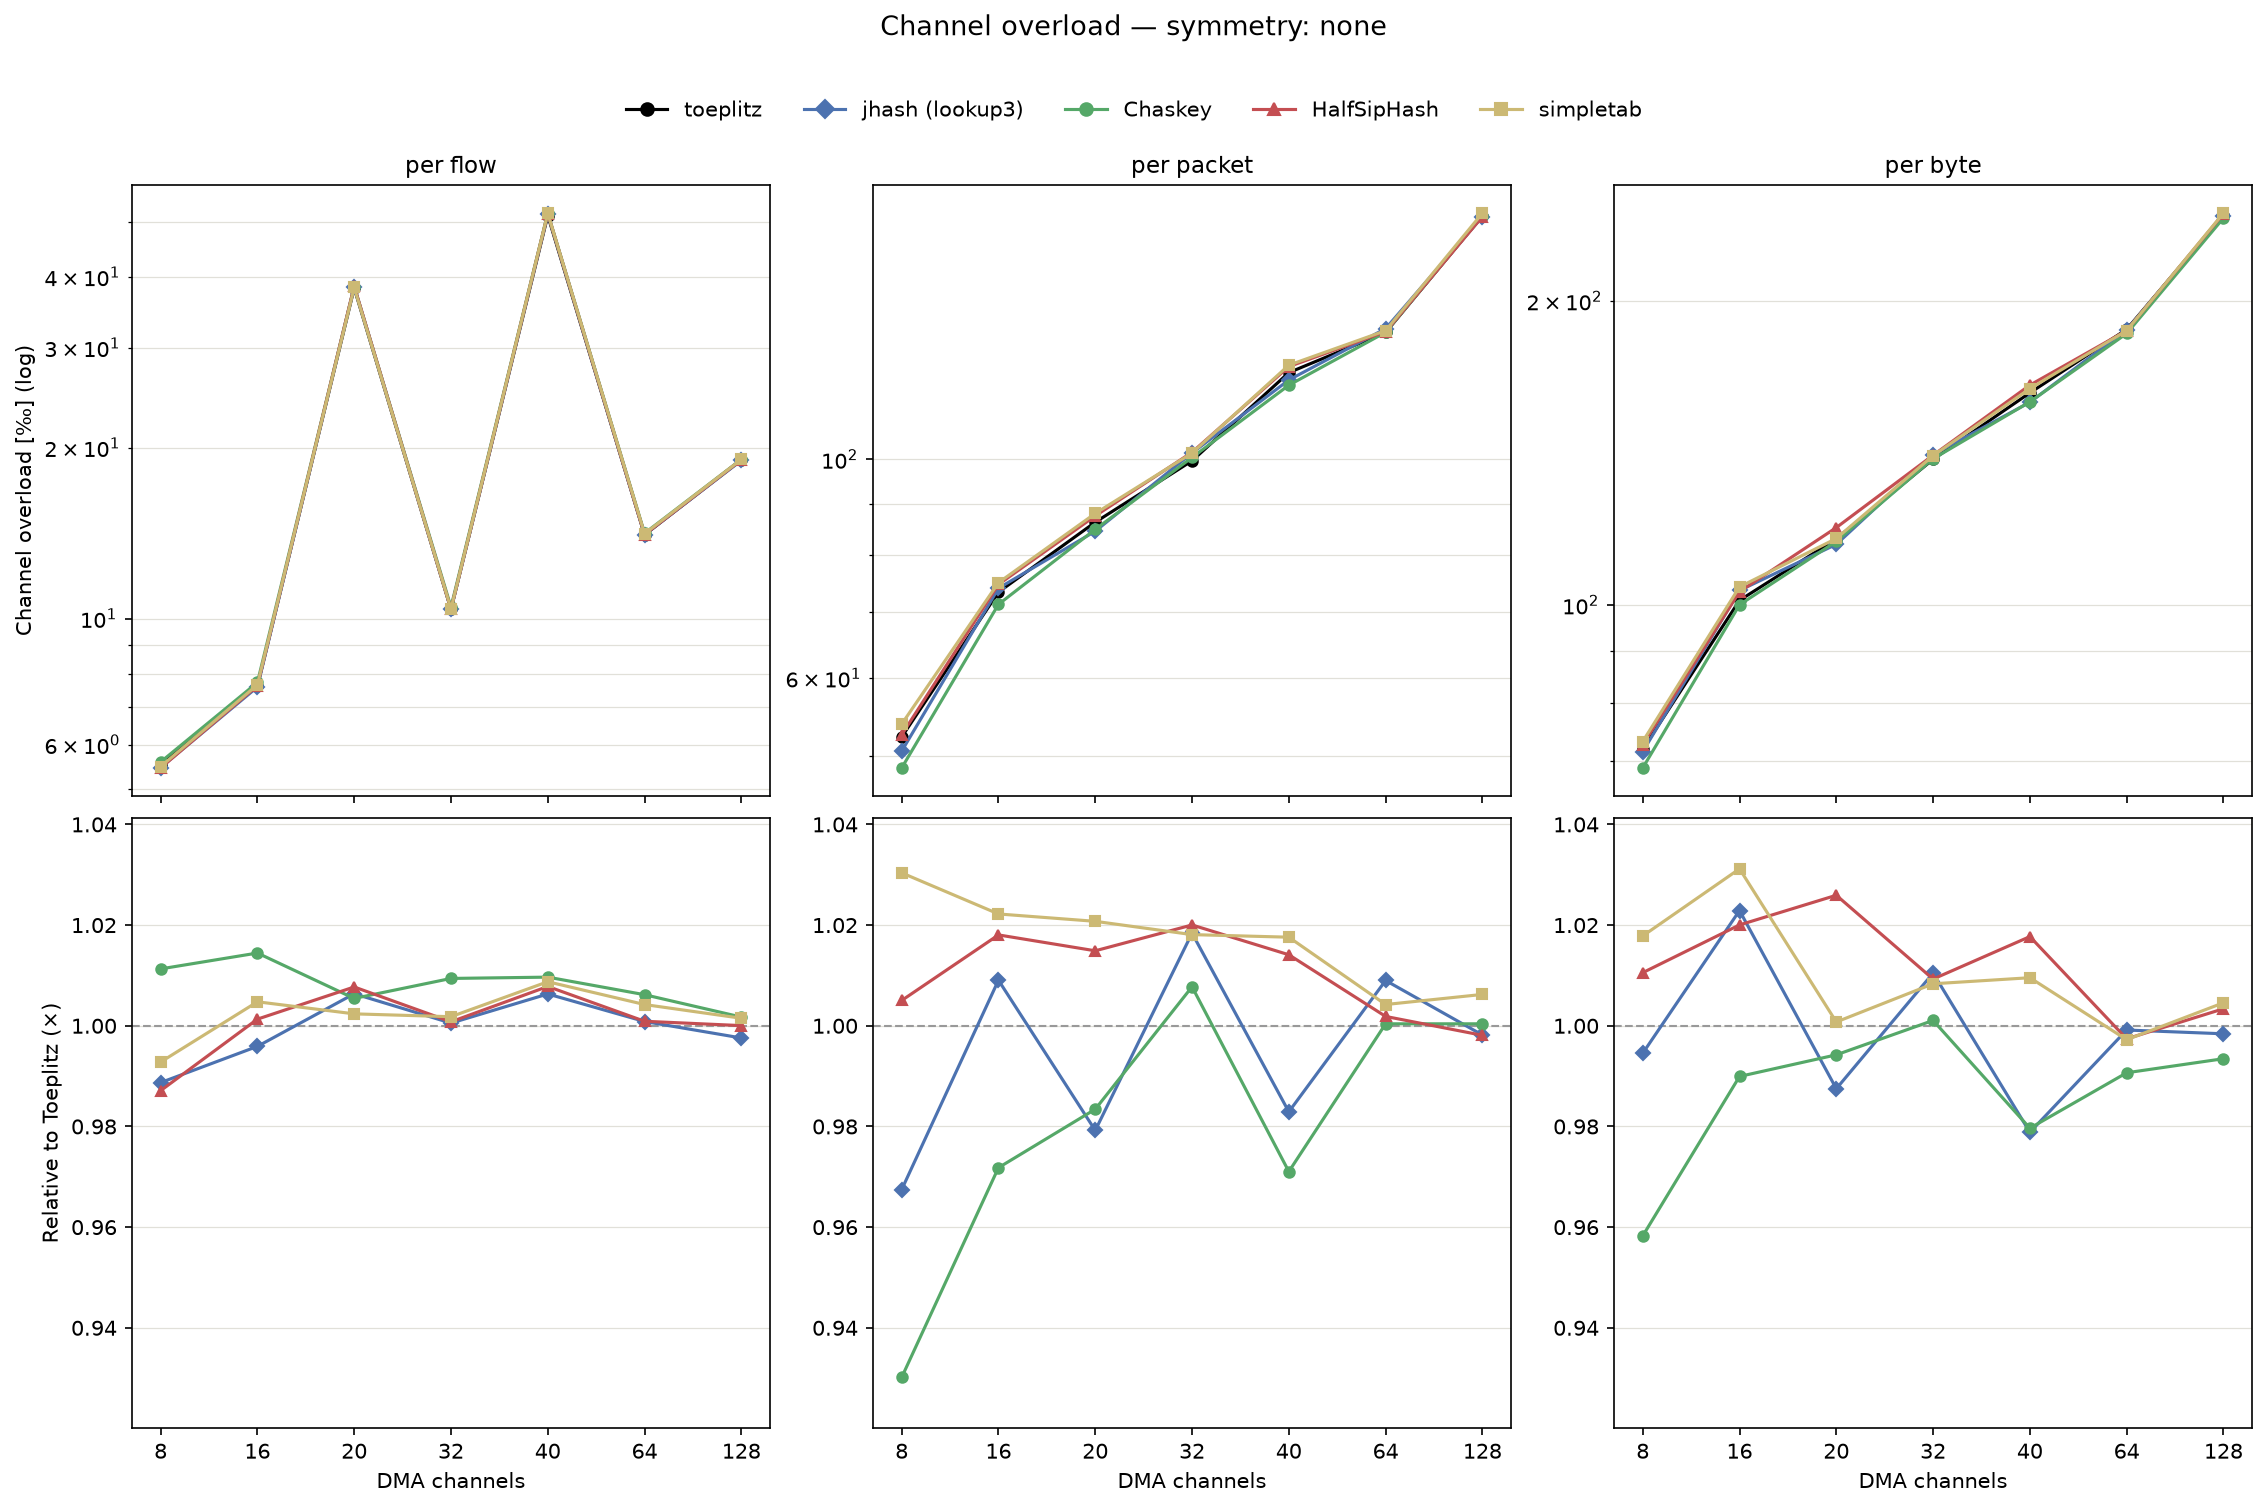
\includegraphics[width=\textwidth]{hashe/overload_none.png}
  \caption{Preťaženie piatich hashovacích funkcií bez symetrie (hore) a ich pomer
  k~Toeplitzu (dole), \texttt{odid1}. \TODO{Prekresliť so slovenskými popismi.}}
  \label{fig:hashe}
\end{figure}

Na obrázku~\ref{fig:hashe} sa krivky funkcií v~hornom riadku takmer prekrývajú. Spodný riadok
rozdiely zväčšuje: priemerná odchýlka od Toeplitzu je 0,5\,\% (flow), 1,6\,\% (packet)
a 1,2\,\% (byte). Najväčší rozdiel je pri 8 kanáloch a váhe \texttt{packet}, kde je Chaskey
o~7,0\,\% \emph{lepší} než Toeplitz. Väčšina odchýlok nemá stabilný smer: napríklad jhash je
pri váhe \texttt{packet} a 8 kanáloch lepší než Toeplitz, ale pri 16 kanáloch horší. Rozdiely sa navyše s~rastúcim počtom
kanálov zmenšujú a pri 128 kanáloch sú všetky funkcie do približne 1\,\% od Toeplitzu.

Pri váhe \texttt{flow} sú krivky prakticky totožné a výrazné špičky pri 20 a 40 kanáloch majú
všetky funkcie rovnaké, lebo ich spôsobuje RETA (sekcia~\ref{sec:reta}).

\subsection{Symetria XOR}

\begin{figure}[ht]
  \centering
  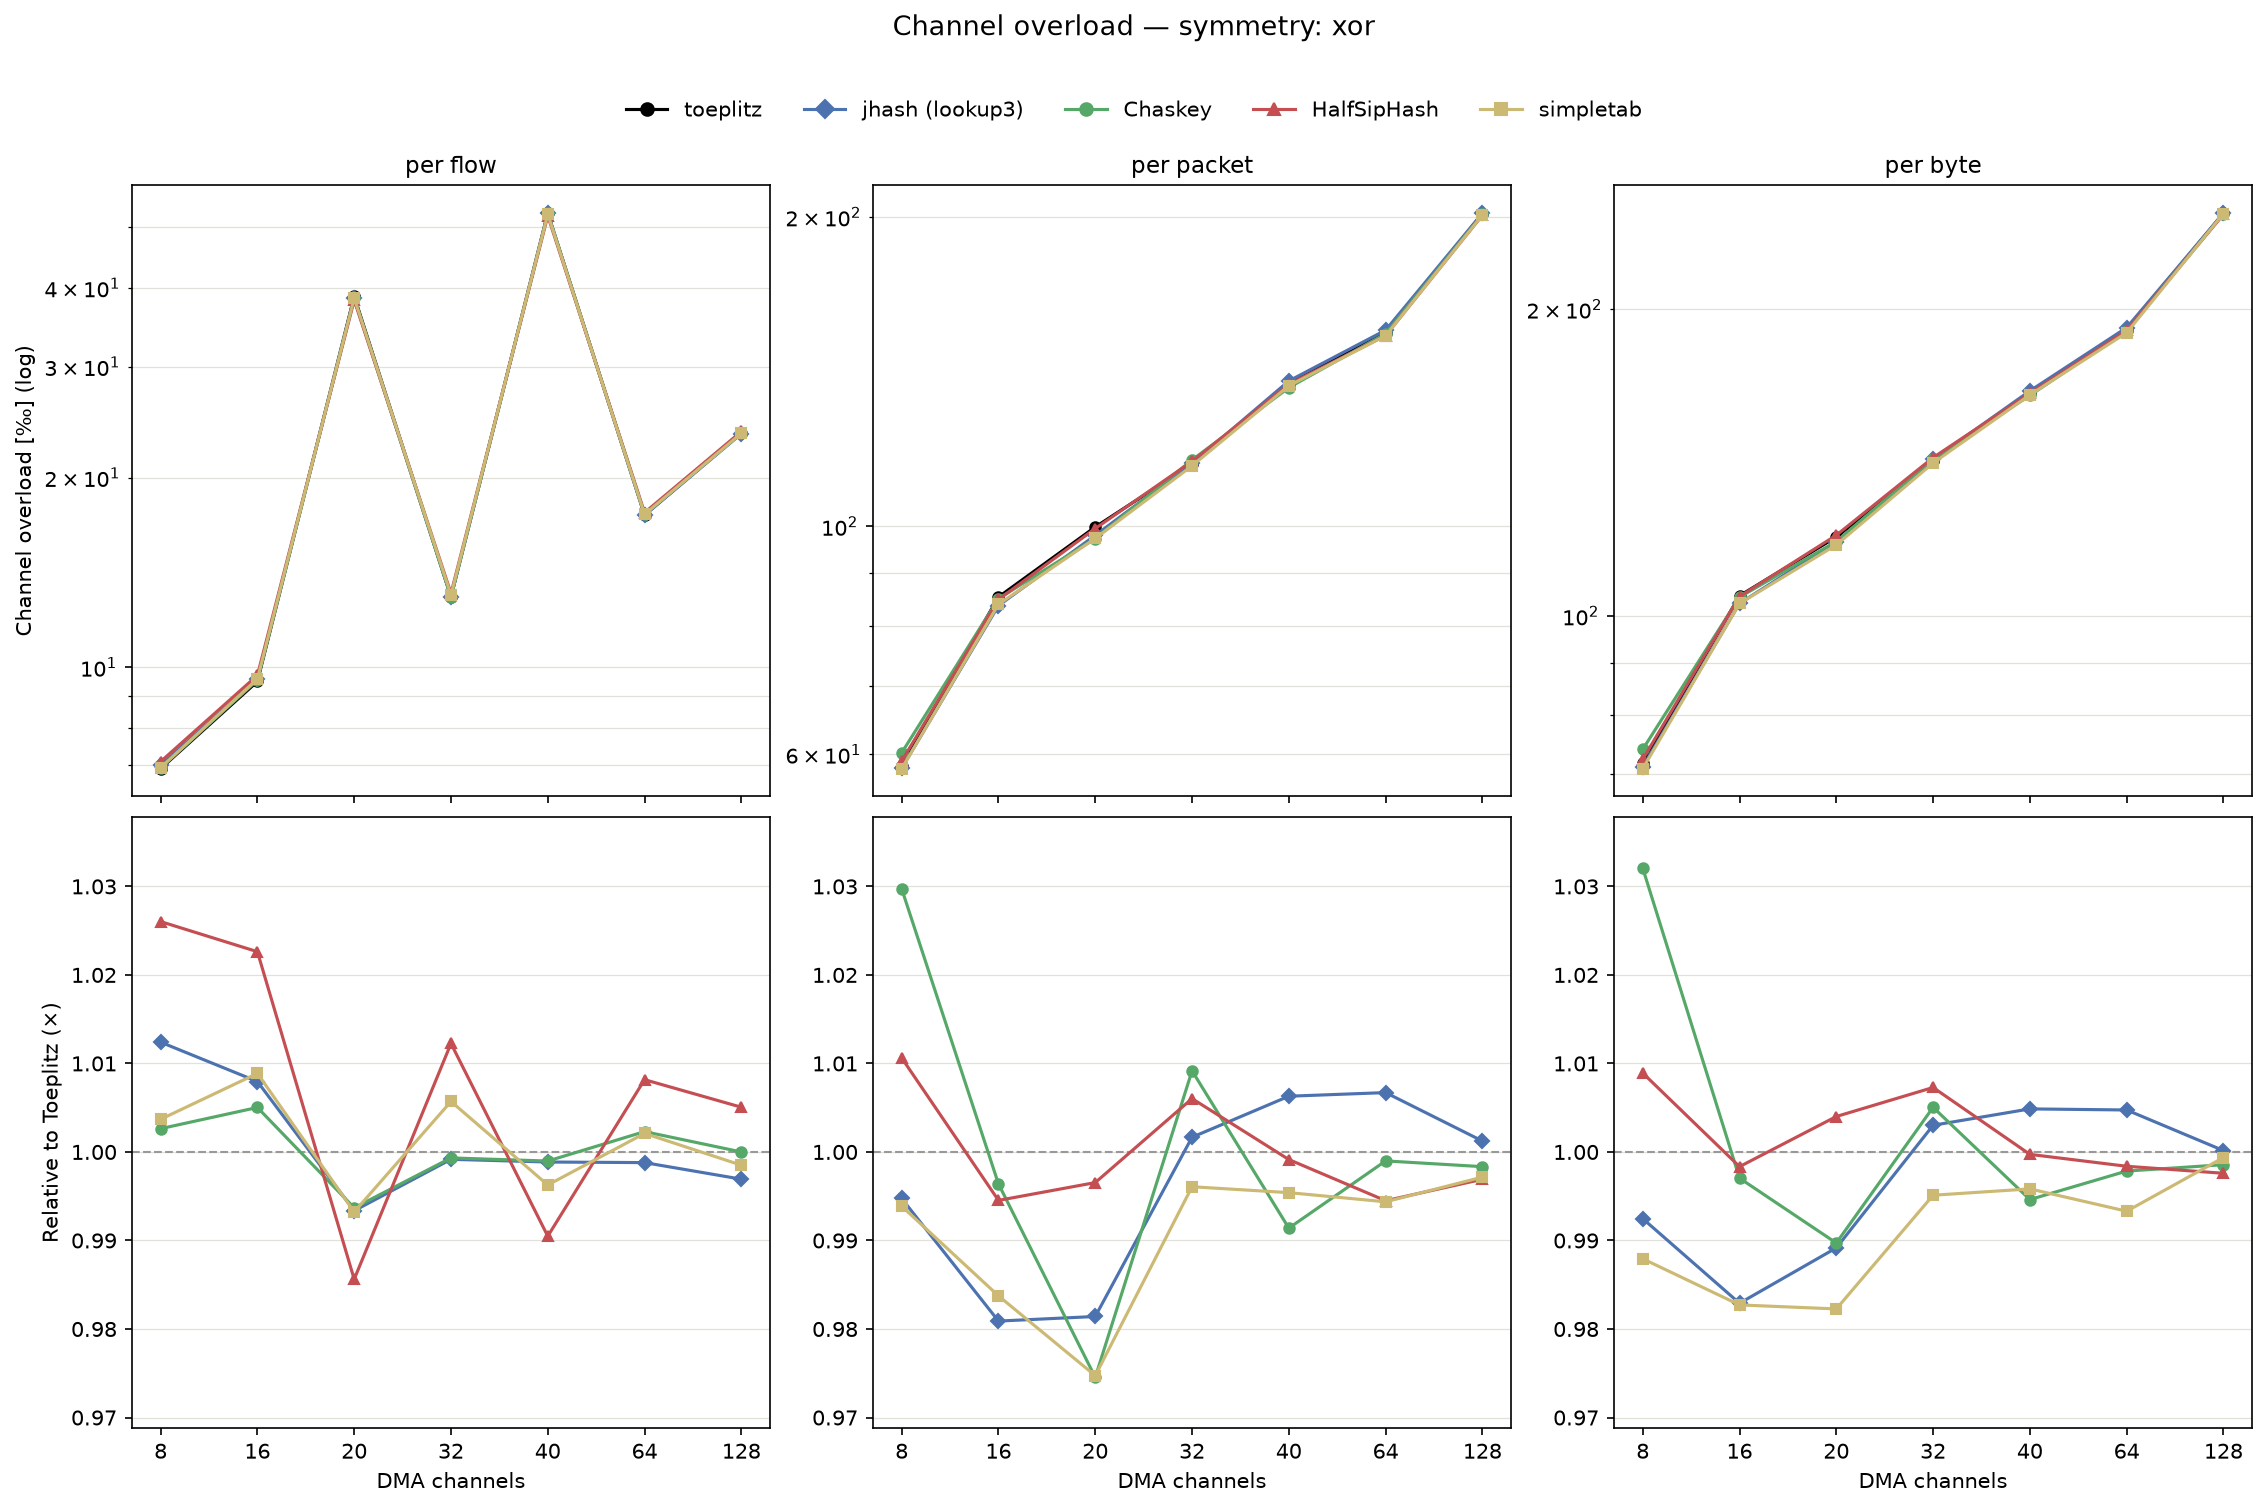
\includegraphics[width=\textwidth]{hashe/overload_xorfold.png}
  \caption{Porovnanie funkcií pri symetrii XOR, \texttt{odid1}.
  \TODO{Prekresliť so slovenskými popismi.}}
  \label{fig:hashe-xor}
\end{figure}

Pri symetrii XOR (obrázok~\ref{fig:hashe-xor}) sú funkcie najbližšie k~sebe. Priemerná
odchýlka je 0,6 až 0,8\,\% a najväčšia 3,2\,\%.

\subsection{Symetria sort}

\begin{figure}[ht]
  \centering
  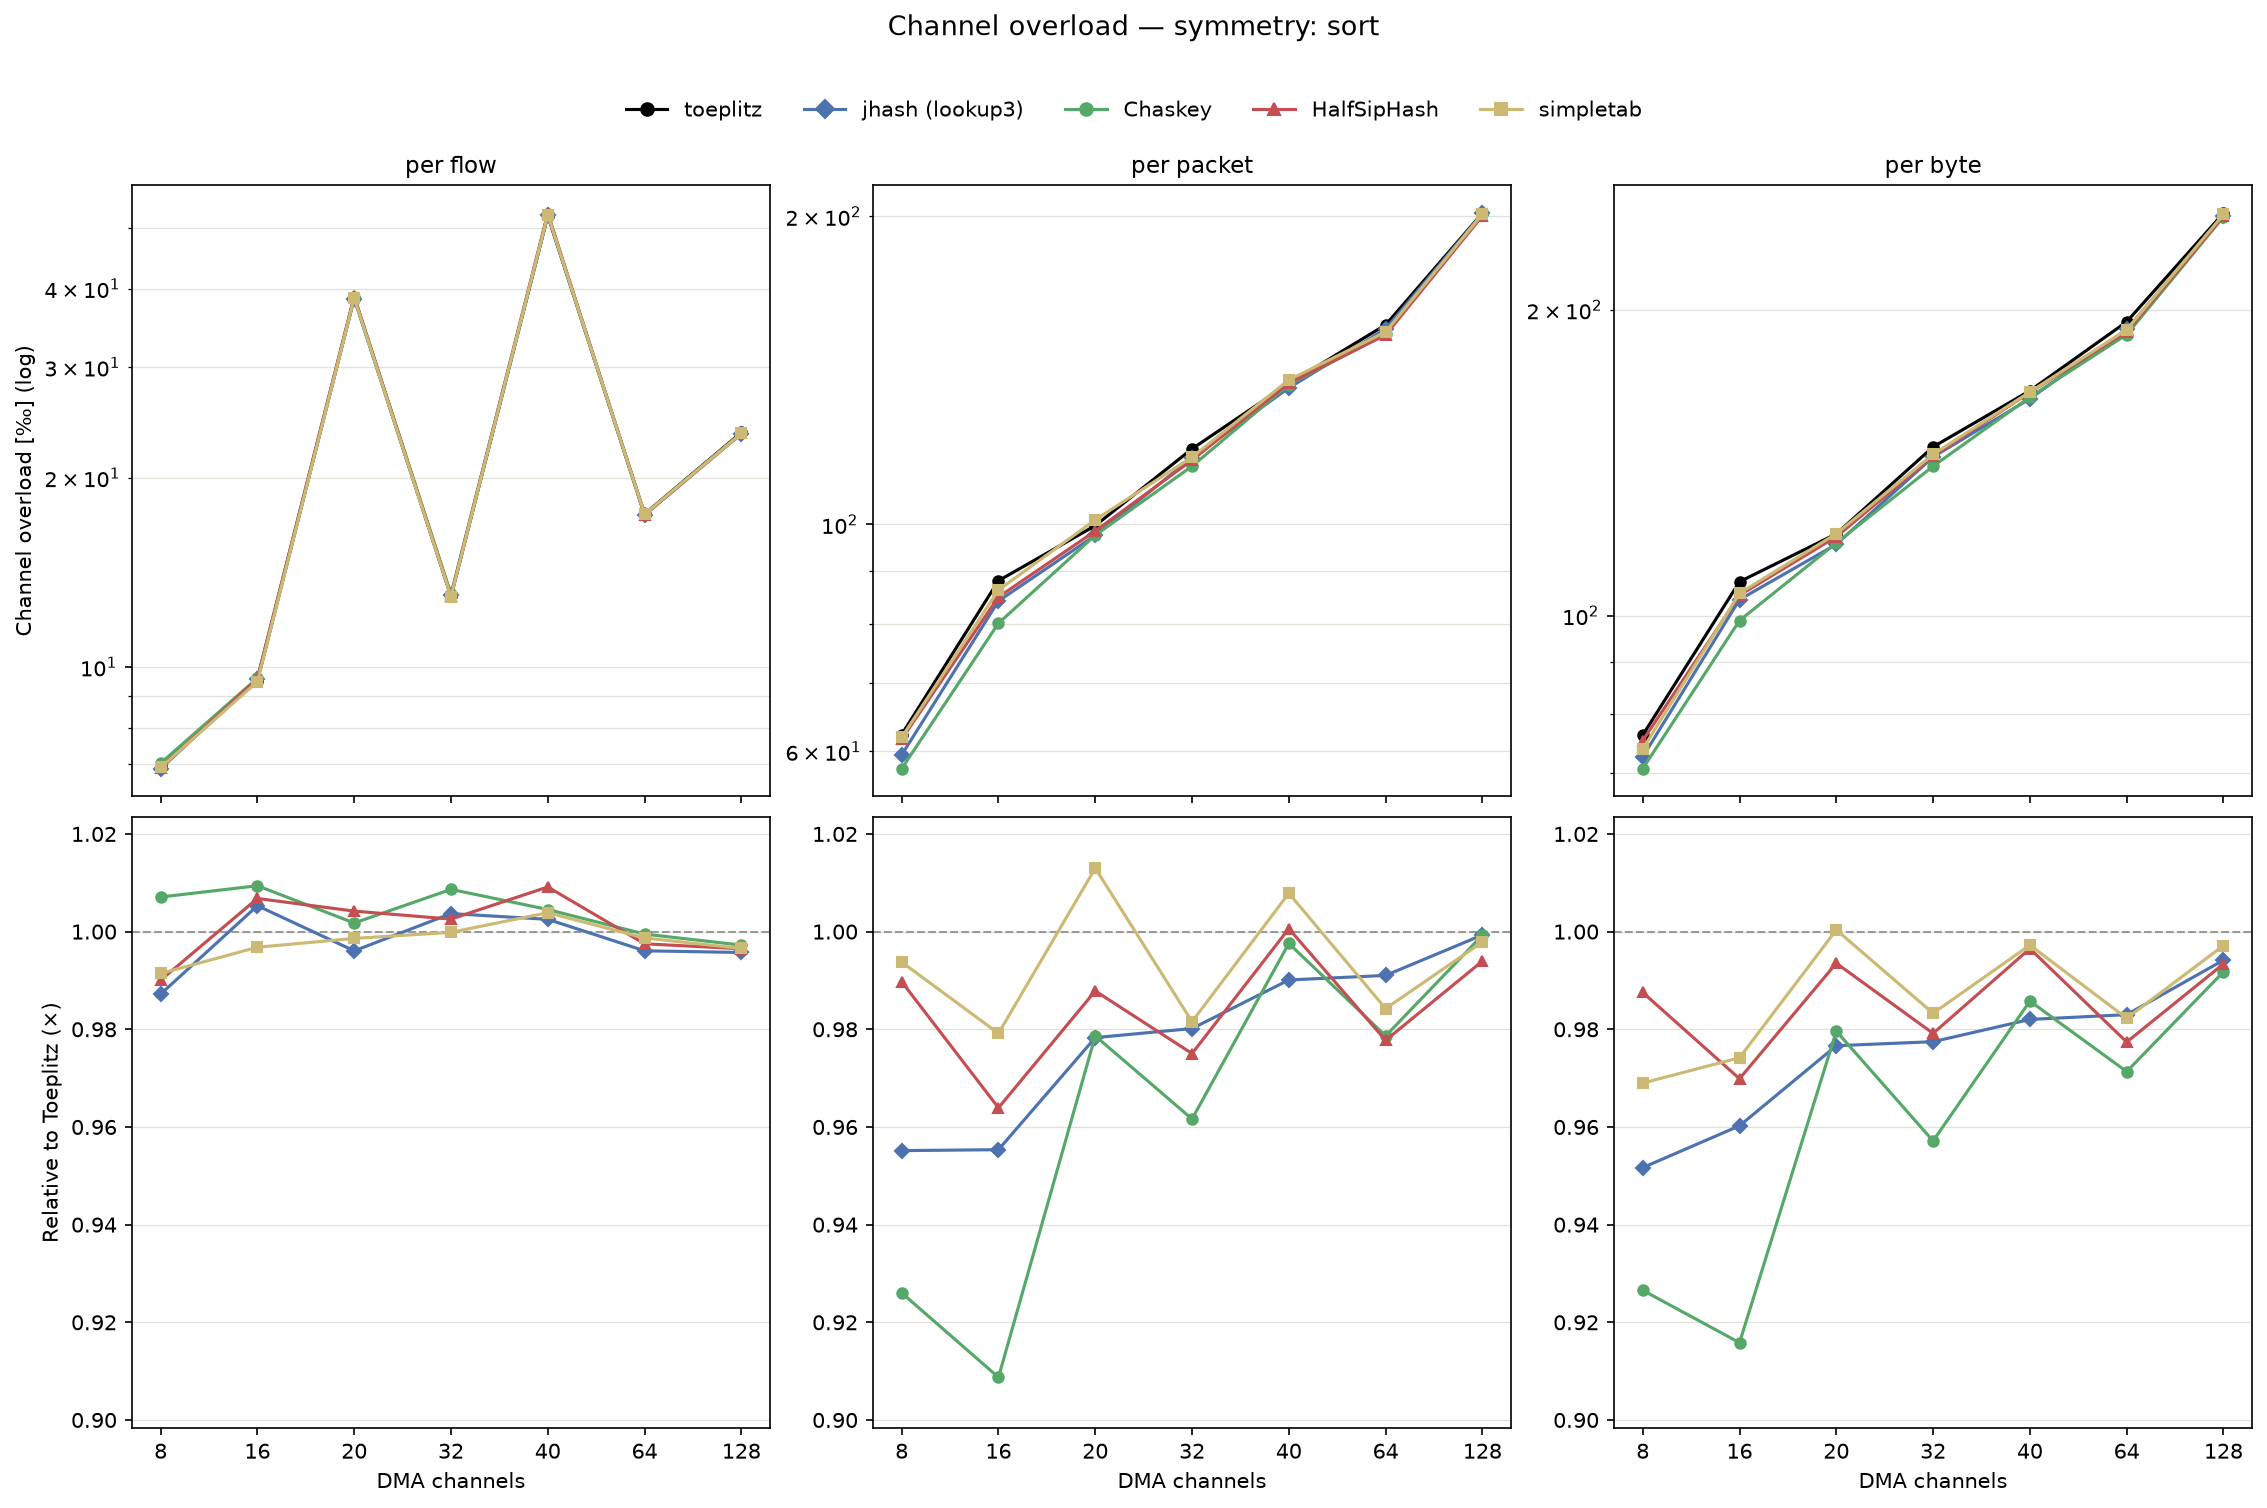
\includegraphics[width=\textwidth]{hashe/overload_sortfold.png}
  \caption{Porovnanie funkcií pri symetrii sort, \texttt{odid1}.
  \TODO{Prekresliť so slovenskými popismi.}}
  \label{fig:hashe-sort}
\end{figure}

Symetria sort je jediný režim, kde sa objavuje náznak systematického rozdielu
(obrázok~\ref{fig:hashe-sort}). Pri váhach \texttt{packet} a \texttt{byte} má Toeplitz
v~priemere najvyššie preťaženie a ostatné funkcie sú pri väčšine počtov kanálov pod ním. Chaskey
je pri 16 kanáloch lepší až o~9,1\,\%. Rozdiel sa s~rastúcim počtom kanálov opäť stráca.
\TODO{Overiť väčším počtom kľúčov, či je to skutočný efekt kombinácie Toeplitz + sort, alebo
náhoda. Toeplitz je lineárny, takže tu môže existovať vysvetlenie.}

\section{Vplyv RSS kľúča}
\label{sec:kluce}

Aby sa dalo posúdiť, či sú rozdiely medzi funkciami významné, treba ich porovnať s~tým, ako
veľmi sa mení výsledok \emph{tej istej} funkcie pri inom náhodnom kľúči.

% !TEX root = ../projekt.tex
\begin{table}[ht]
  \centering
  \small
  \caption{Vplyv kľúča bez symetrie, \texttt{odid1}, hodnoty v~\textperthousand. \emph{Toeplitz}: najlepší až najhorší zo 16 kľúčov. \emph{Hashe}: rozpätie priemerov piatich funkcií. \emph{Kľúče}: priemerné rozpätie medzi kľúčmi jednej funkcie.}
  \label{tab:kluce}
  \begin{tabular}{r rrrr rrrr}
    \toprule
    & \multicolumn{4}{c}{packet} & \multicolumn{4}{c}{byte} \\
    Kanály & Toeplitz & hashe & kľúče & pomer & Toeplitz & hashe & kľúče & pomer \\
    \midrule
    8 & 41,9--71,3 & 5,2 & 21,0 & 4,0$\times$ & 60,1--96,0 & 4,3 & 27,9 & 6,5$\times$ \\
    16 & 61,0--83,1 & 3,7 & 18,5 & 5,0$\times$ & 86,8--116,0 & 4,2 & 26,2 & 6,3$\times$ \\
    20 & 75,9--95,5 & 3,6 & 20,9 & 5,8$\times$ & 101,7--128,3 & 4,5 & 25,6 & 5,7$\times$ \\
    32 & 91,6--108,4 & 2,0 & 16,6 & 8,3$\times$ & 128,8--151,1 & 1,5 & 21,1 & 14,4$\times$ \\
    40 & 106,2--133,4 & 5,7 & 22,2 & 3,9$\times$ & 140,7--173,4 & 6,3 & 29,0 & 4,6$\times$ \\
    64 & 127,9--143,2 & 1,2 & 15,0 & 12,4$\times$ & 178,2--201,0 & 1,7 & 20,2 & 11,6$\times$ \\
    128 & 170,2--183,5 & 1,4 & 12,6 & 8,8$\times$ & 235,8--251,0 & 2,7 & 15,4 & 5,7$\times$ \\
    \bottomrule
  \end{tabular}
\end{table}


Tabuľka~\ref{tab:kluce} ukazuje, že kľúč má väčší vplyv než výber funkcie pri každom počte
kanálov: rozpätie medzi kľúčmi je 3,9 až 12,4-krát väčšie pri váhe \texttt{packet} a 4,6 až
14,4-krát pri váhe \texttt{byte}. Pri malom počte kanálov je vplyv kľúča veľký aj absolútne.
Toeplitz s~8 kanálmi má pri váhe \texttt{packet} podľa kľúča preťaženie od 41,9 do
71,3\,\textperthousand, teda jeho najhorší kľúč je o~70\,\% horší než najlepší. Pravdepodobným dôvodom je, že pri
málo kanáloch rozhoduje, či najväčšie toky padnú do toho istého kanála.
\TODO{Overiť: pozrieť, kam padnú najväčšie toky pri najlepšom a najhoršom kľúči.}

\begin{figure}[p]
  \centering
  \begin{subfigure}{0.54\textwidth}
    \centering
    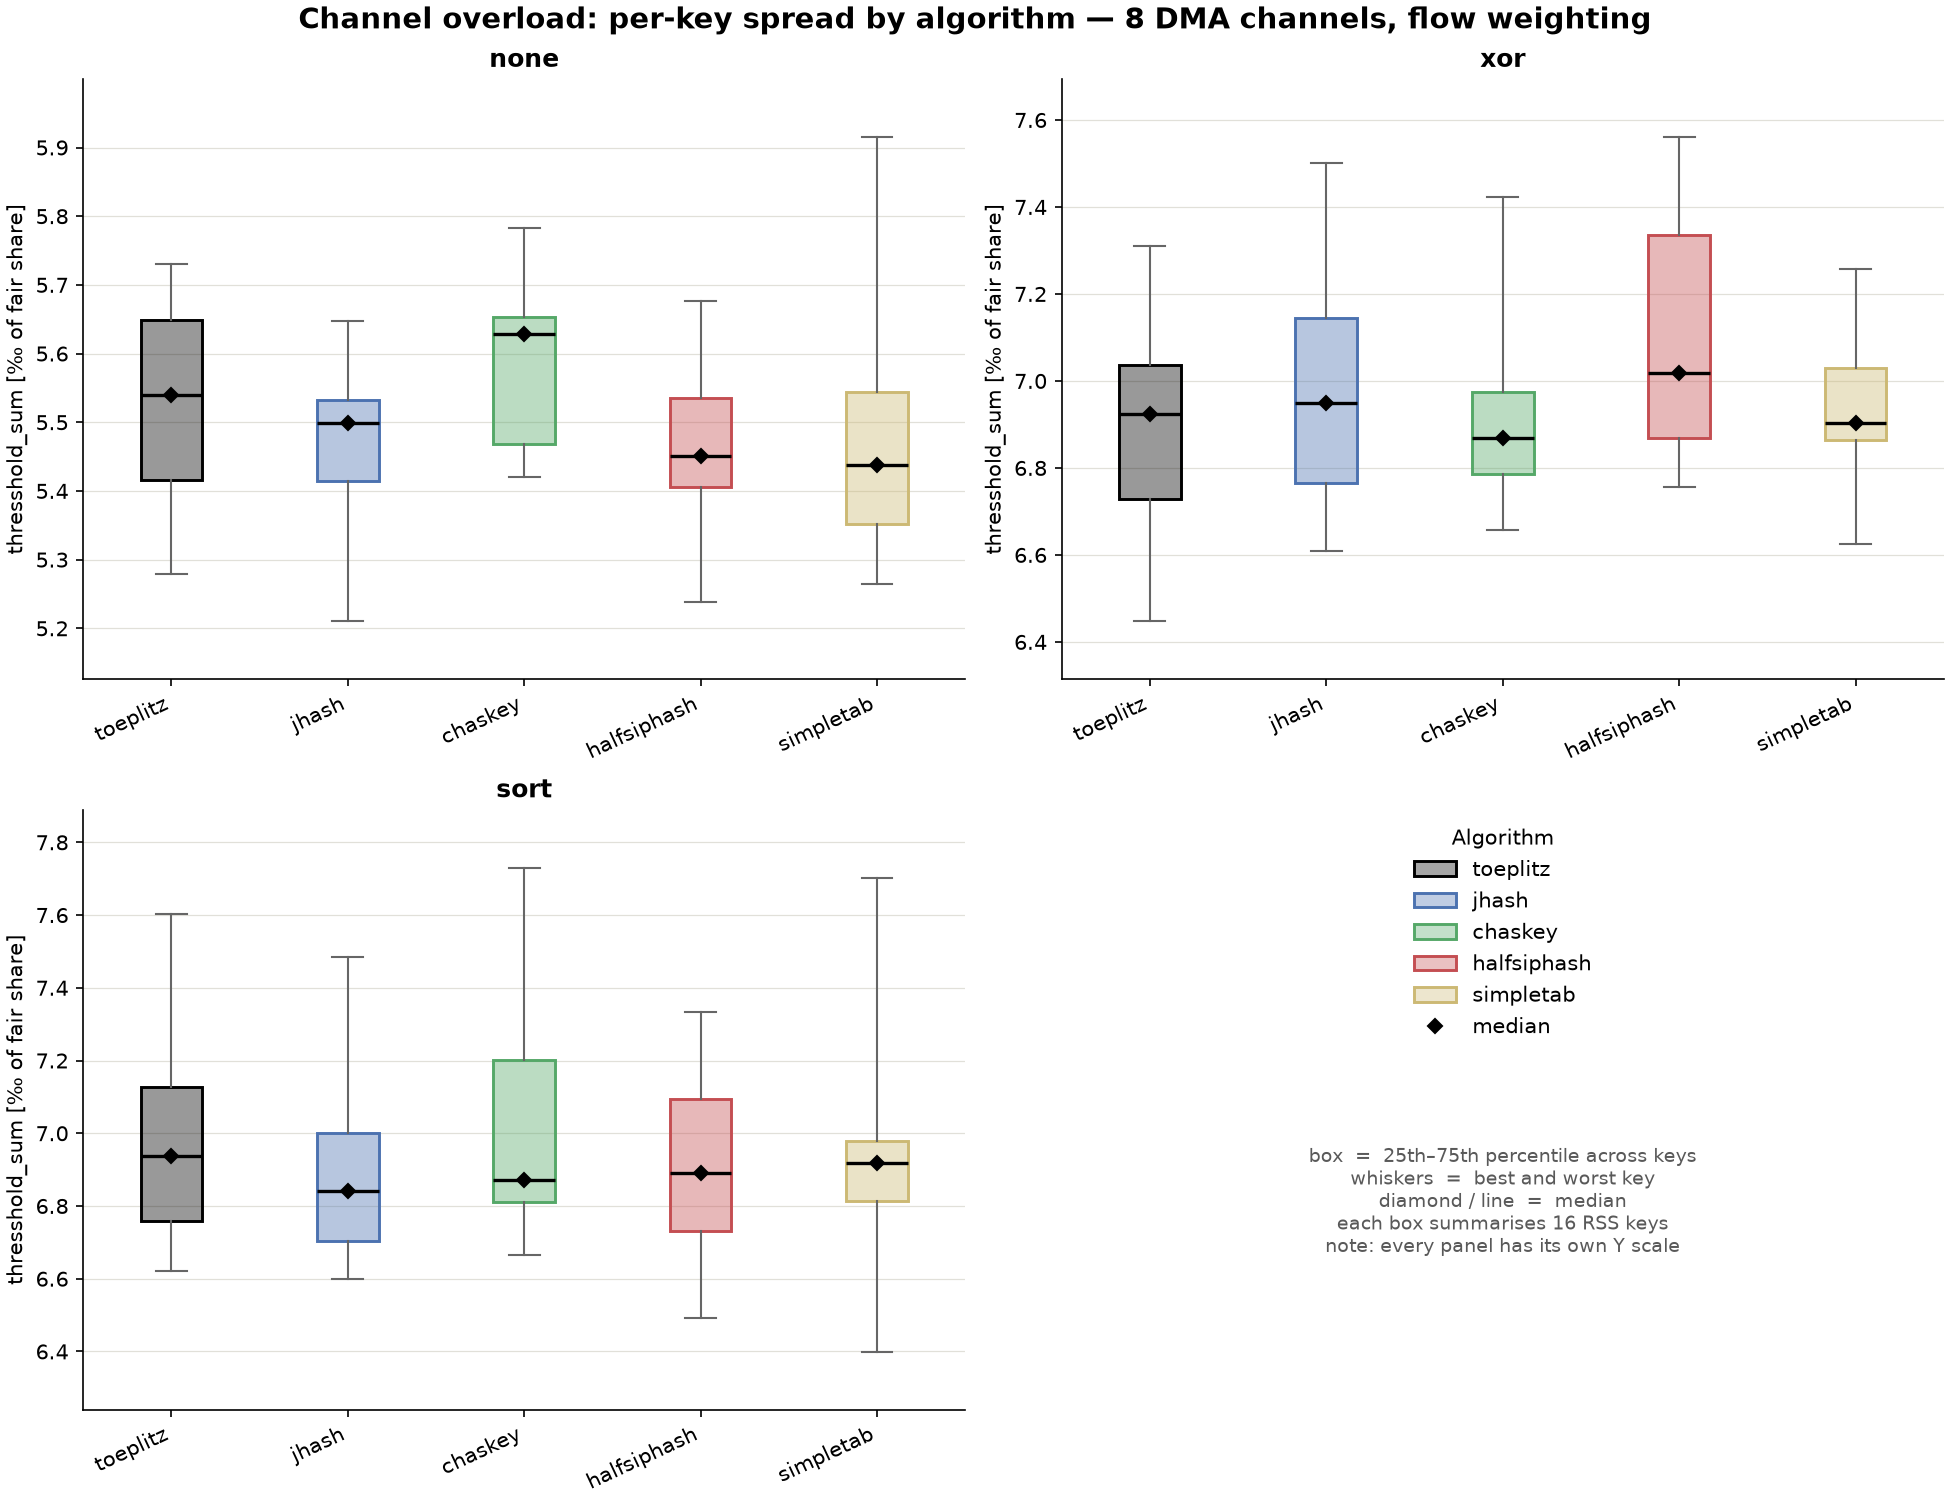
\includegraphics[width=\textwidth]{kluce/keys_8.png}
    \caption{8 kanálov}
  \end{subfigure}

  \begin{subfigure}{0.54\textwidth}
    \centering
    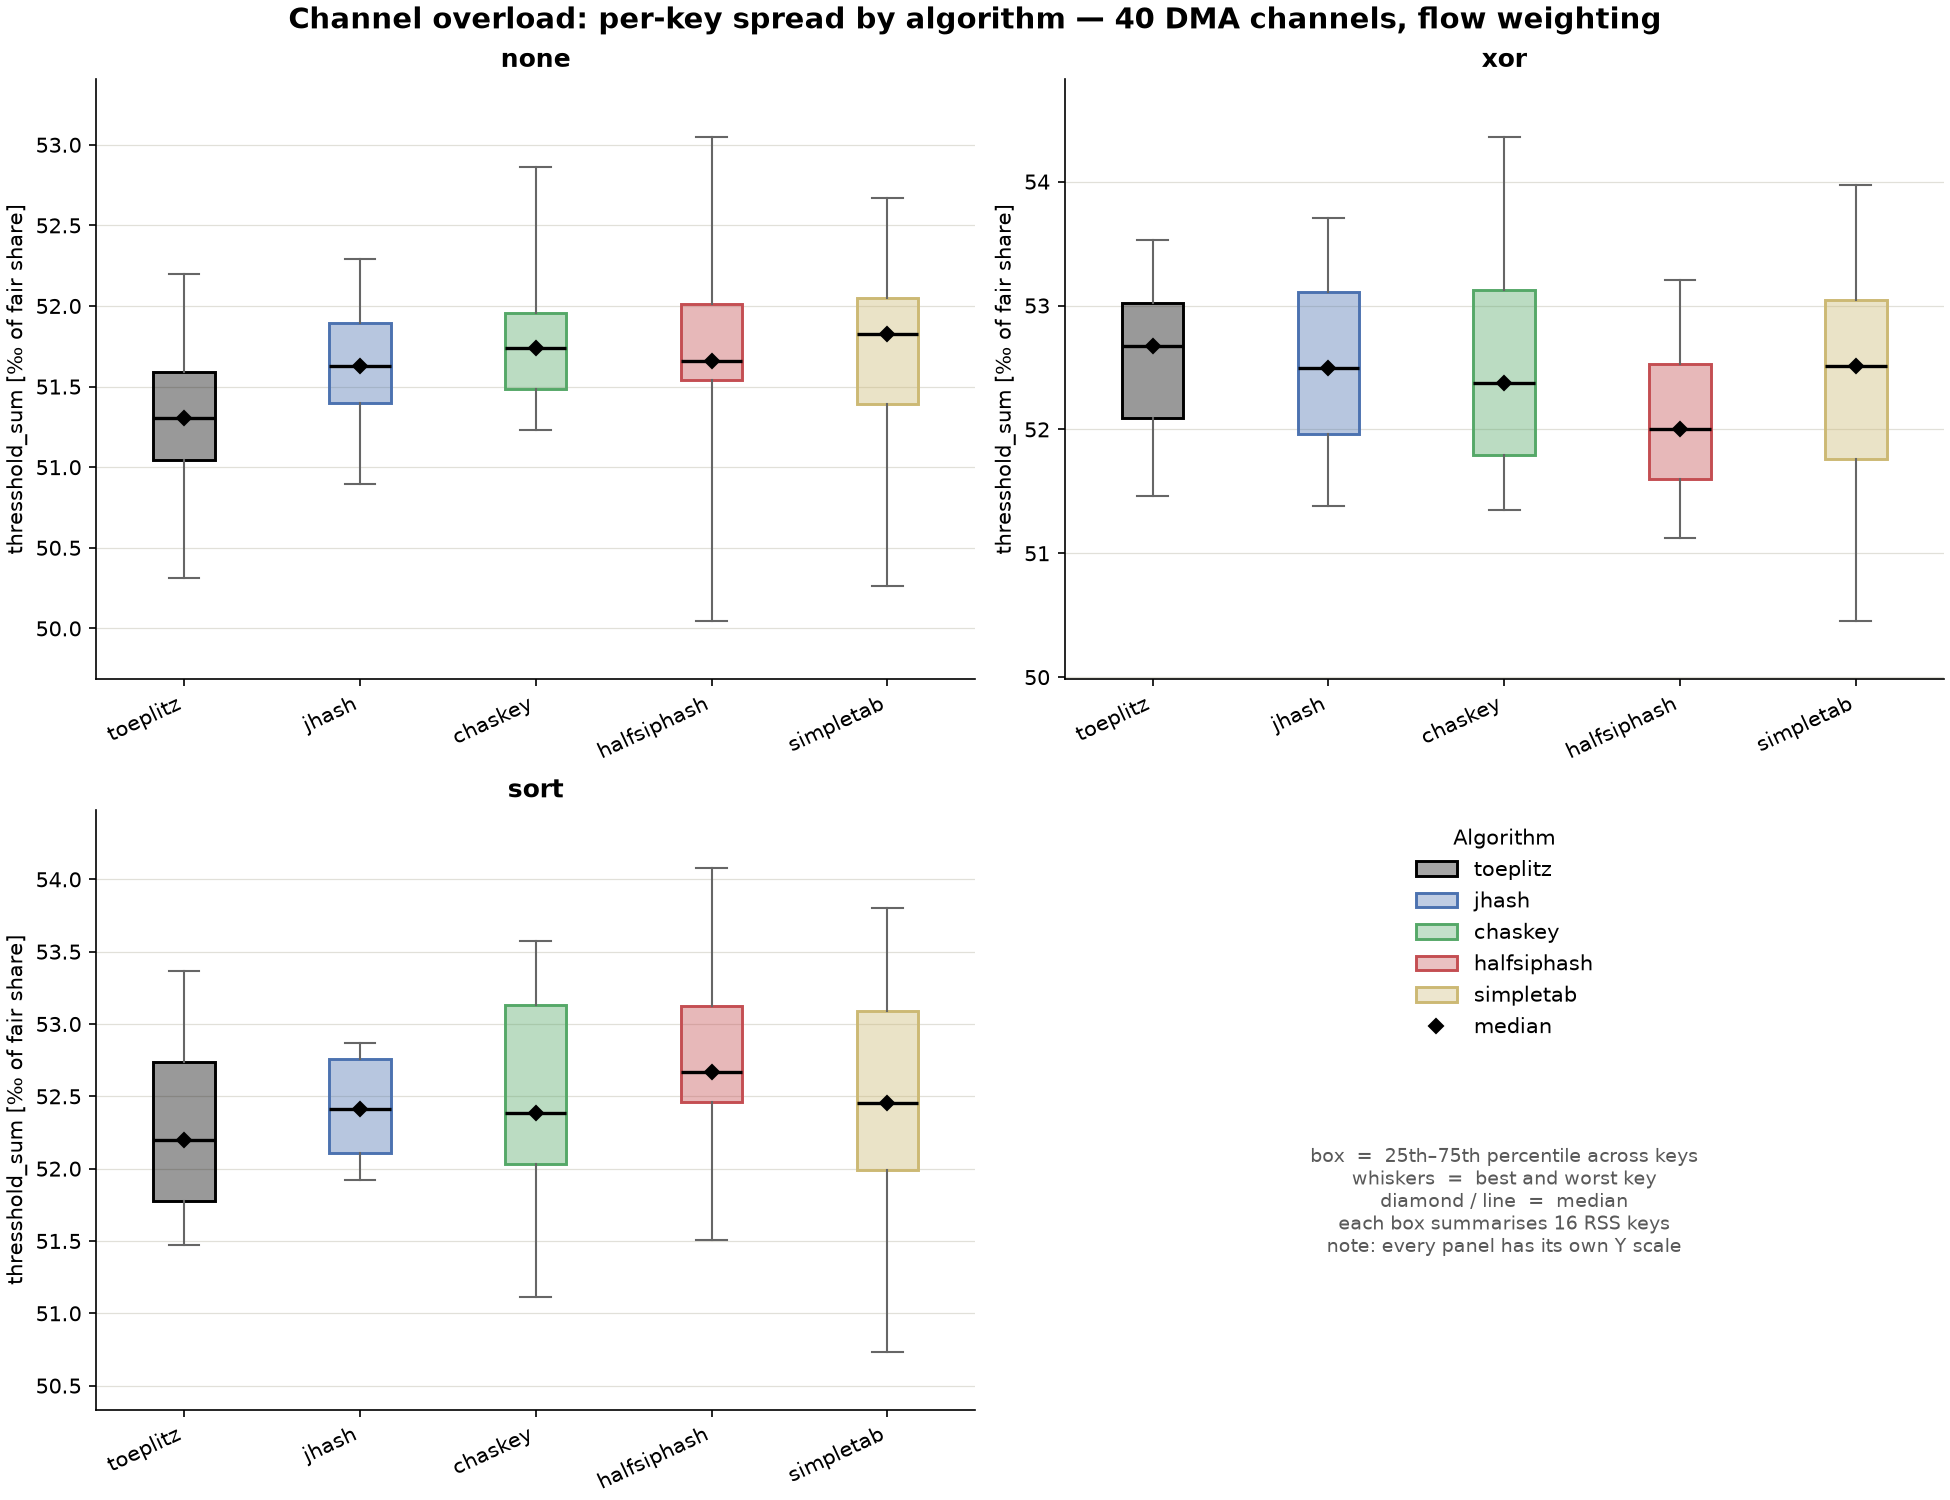
\includegraphics[width=\textwidth]{kluce/keys_40.png}
    \caption{40 kanálov}
  \end{subfigure}

  \begin{subfigure}{0.54\textwidth}
    \centering
    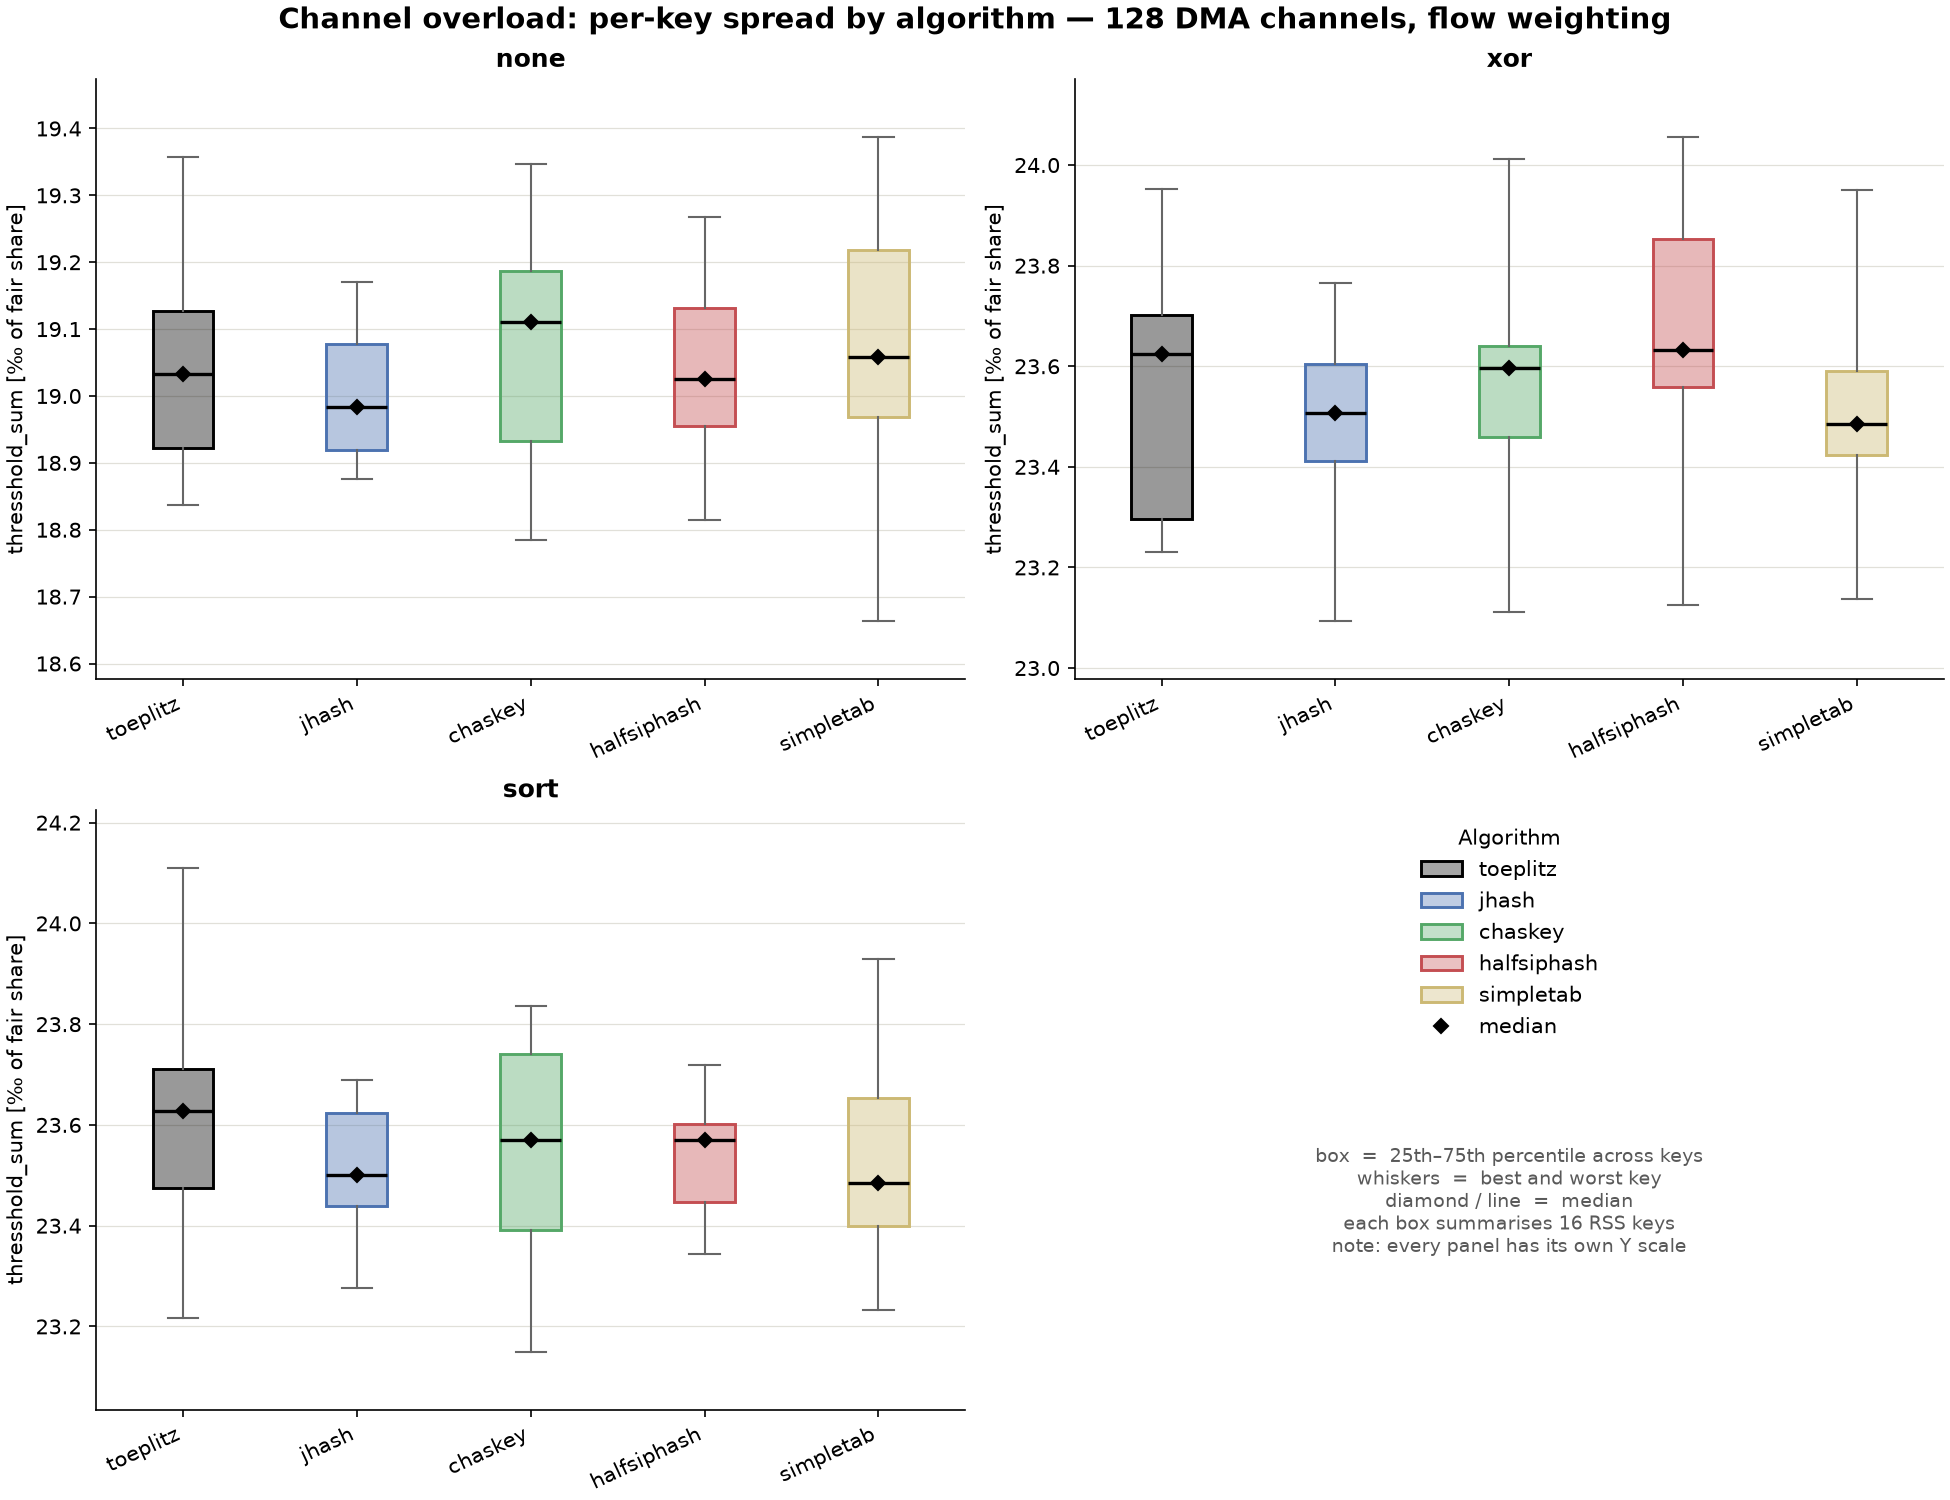
\includegraphics[width=\textwidth]{kluce/keys_128.png}
    \caption{128 kanálov}
  \end{subfigure}
  \caption{Rozptyl preťaženia medzi 16 kľúčmi pri váhe \texttt{flow}, \texttt{odid1}. Škatuľa
  je 25.--75.~percentil, fúzy sú najlepší a najhorší kľúč. Každý panel má vlastnú os Y.
  \TODO{Prekresliť so slovenskými popismi.}}
  \label{fig:kluce}
\end{figure}

Obrázok~\ref{fig:kluce} zobrazuje rozloženie cez kľúče pri váhe \texttt{flow}, kde sa meria čistá
kvalita hashu bez vplyvu veľkých tokov. Škatule všetkých funkcií sa vo všetkých režimoch
prekrývajú, takže podľa rozloženia cez kľúče nemožno žiadnu funkciu označiť za lepšiu.
Pozor na mierku: pri 8 kanáloch je celý rozsah Toeplitzu bez symetrie iba 5,3 až
5,7\,\textperthousand{} a pri 128 kanáloch 18,8 až 19,4\,\textperthousand.

\emph{Poznámka:} výber ,,najlepšieho`` kľúča na tých istých dátach by bol zavádzajúci. Dobrý
kľúč je výhodný preto, ako práve rozdelil konkrétne veľké toky, a na inej prevádzke výhodu stratí.
\TODO{Dalo by sa overiť: vybrať najlepší kľúč na jednej vzorke a zmerať ho na inej.}

\section{Štatistické vyhodnotenie}
\label{sec:statistika}

\begin{itemize}
  \item \textbf{Kľúč oproti funkcii.} Cez všetkých 63 konfigurácií (3 symetrie, 3 váhy, 7 počtov
        kanálov) je rozpätie medzi kľúčmi v~mediáne 6,6-krát väčšie než rozpätie medzi
        funkciami (od 3,1 do 23,1-krát).
  \item \textbf{Permutačný test.} Hodnoty kľúčov sme náhodne premiešali medzi funkciami
        (3\,000 permutácií) a testovali, či je skutočný rozdiel funkcií väčší než náhodný.
        $p<0{,}05$ vyšlo v~4 z~63 konfigurácií, čisto náhodou by sa očakávali približne 3.
        Žiadna konfigurácia nemá $p<0{,}01$. Všetky štyri sú pri symetrii \emph{sort}, čo
        zodpovedá náznaku z~obrázka~\ref{fig:hashe-sort}.
  \item \textbf{Podiel vysvetleného rozptylu.} Voľba funkcie vysvetľuje najviac približne
        14\,\% rozptylu výsledkov ($\eta^2$, obrázok~\ref{fig:spread}), väčšinou menej než 10\,\%.
\end{itemize}

\begin{figure}[ht]
  \centering
  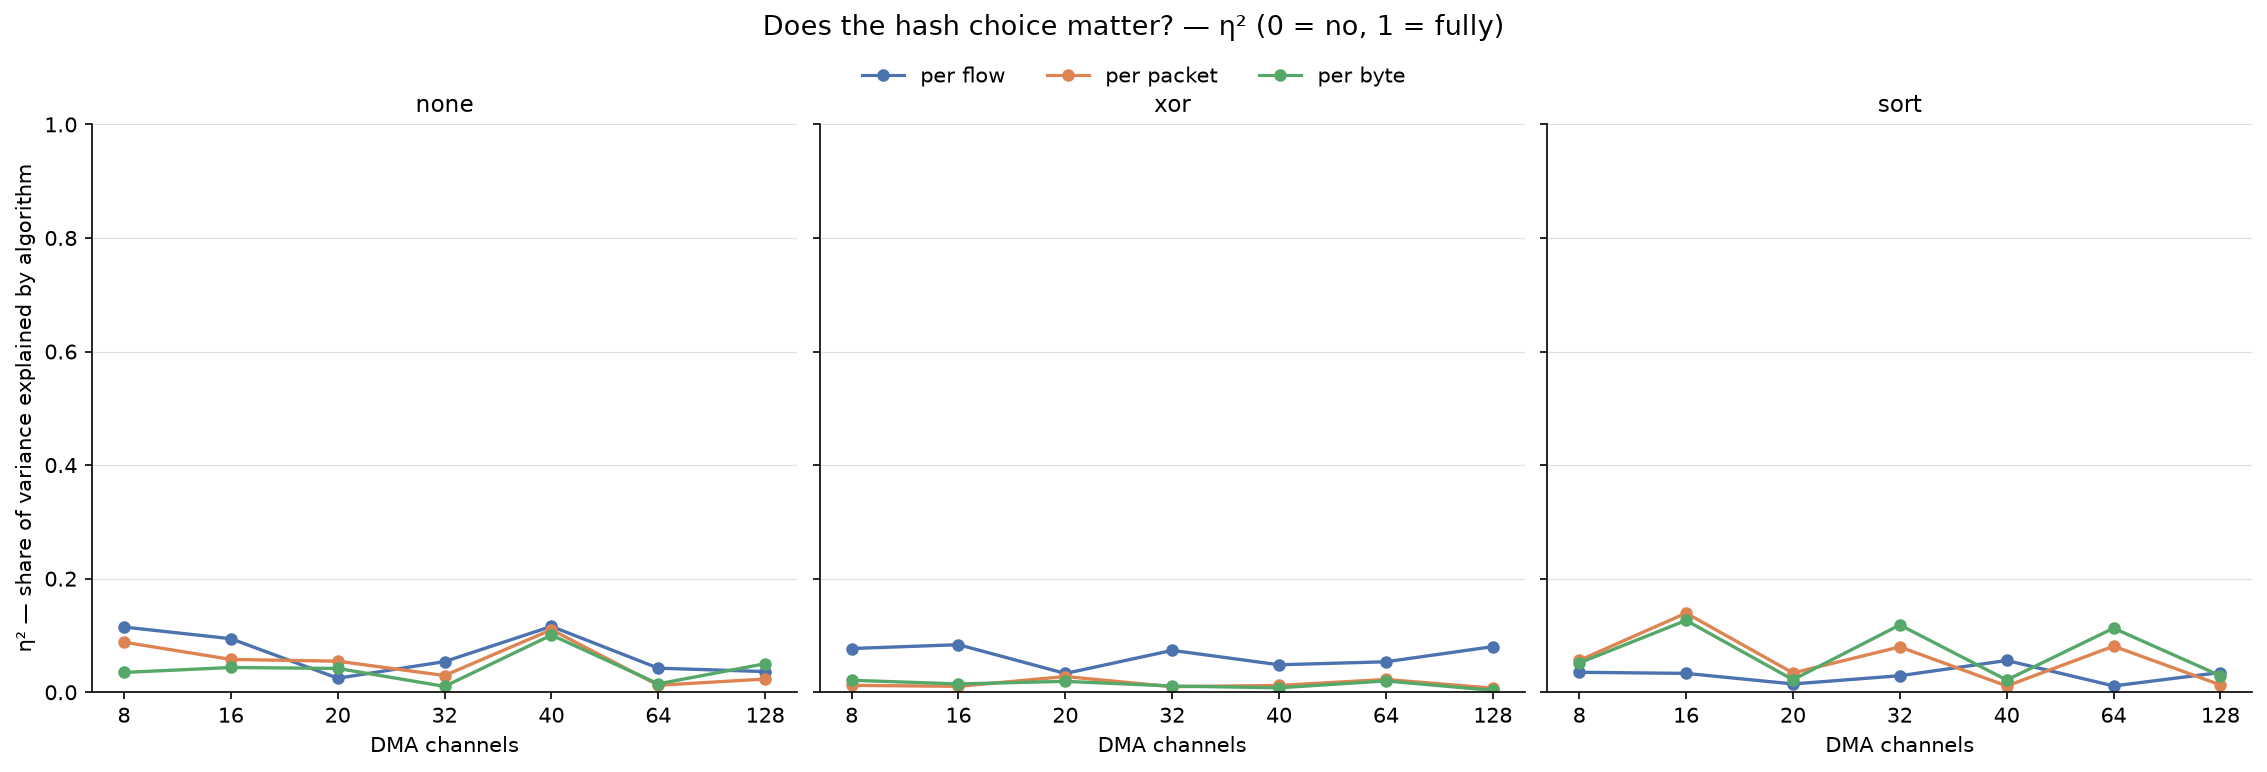
\includegraphics[width=\textwidth]{hashe/spread.png}
  \caption{Podiel rozptylu vysvetlený voľbou hashovacej funkcie ($\eta^2$), \texttt{odid1}.
  \TODO{Prekresliť so slovenskými popismi.}}
  \label{fig:spread}
\end{figure}

\paragraph{Záver porovnania.} Na vzorke \texttt{odid1} s~plným tuple sa medzi piatimi funkciami
nepreukázal rozdiel, ktorý by prevýšil vplyv náhodného kľúča. Výmena kvalitného hashu preto
nerieši nerovnomernú záťaž. Sekcia~\ref{sec:dalsie-vzorky} ukazuje dôležitú výnimku:
slabšia funkcia môže byť horšia, keď má vstup málo entropie. Ďalšie experimenty používajú Toeplitz.

\section{Cena symetrie}
\label{sec:cena-symetrie}

% !TEX root = ../projekt.tex
\begin{table}[ht]
  \centering
  \small
  \caption{Zmena preťaženia Toeplitzu po zapnutí symetrie oproti \texttt{none}, cez 7 počtov kanálov.}
  \label{tab:symetria}
  \begin{tabular}{l rr rr}
    \toprule
    & \multicolumn{2}{c}{XOR} & \multicolumn{2}{c}{sort} \\
    Váha & priemer [\%] & rozsah [\%] & priemer [\%] & rozsah [\%] \\
    \midrule
    flow & +18,1 & +1,5 až +25,0 & +18,3 & +1,3 až +26,3 \\
    packet & +14,3 & +11,8 až +16,4 & +16,7 & +12,2 až +20,1 \\
    byte & +2,0 & -0,4 až +3,6 & +4,4 & +2,4 až +6,9 \\
    \bottomrule
  \end{tabular}
\end{table}


Symetria zlúči oba smery spojenia do jedného kanála, čím vznikajú väčšie jednotky záťaže.
Podľa tabuľky~\ref{tab:symetria} zvyšuje preťaženie pri váhach \texttt{flow} a \texttt{packet}
priemerne o~14 až 18\,\%, pri váhe \texttt{byte} iba o~2 až 4\,\%.
\TODO{Vysvetliť, prečo je cena pri bajtoch nižšia. Hypotéza: bajty sú v~jednom smere toku,
ten druhý k~záťaži pridá málo. Treba overiť na dátach.}

\section{Vplyv tabuľky RETA}

Pri 20 a 40 kanáloch tvorí preťaženie vo váhe \texttt{flow} takmer výlučne kvantizácia RETA
(sekcia~\ref{sec:reta}): teoreticky 37,5 a 50,0\,\textperthousand, namerané 38,2 a
51,3\,\textperthousand. Pri mocninách dvoch tento efekt neexistuje.

\section{Koľko sa dá získať pri zachovaní afinity toku}
\label{sec:hranica}

% !TEX root = ../projekt.tex
\begin{table}[ht]
  \centering
  \small
  \caption{Preťaženie [\textperthousand]: Toeplitz a orákulum JSQ, pevné okno, \texttt{odid1}.}
  \label{tab:jsq}
  \begin{tabular}{r rrr rrr}
    \toprule
    & \multicolumn{3}{c}{packet} & \multicolumn{3}{c}{byte} \\
    Kanály & Toeplitz & JSQ & zmena & Toeplitz & JSQ & zmena \\
    \midrule
    8 & 52,3 & 6,1 & $-88$\,\% & 72,0 & 12,0 & $-83$\,\% \\
    16 & 73,3 & 12,1 & $-84$\,\% & 101,0 & 22,8 & $-77$\,\% \\
    20 & 86,3 & 14,4 & $-83$\,\% & 116,3 & 26,8 & $-77$\,\% \\
    32 & 99,6 & 20,8 & $-79$\,\% & 139,4 & 35,8 & $-74$\,\% \\
    40 & 122,4 & 22,9 & $-81$\,\% & 162,2 & 41,0 & $-75$\,\% \\
    64 & 134,4 & 32,2 & $-76$\,\% & 187,4 & 54,8 & $-71$\,\% \\
    128 & 176,5 & 50,3 & $-71$\,\% & 243,2 & 89,4 & $-63$\,\% \\
    \bottomrule
  \end{tabular}
\end{table}


\begin{figure}[ht]
  \centering
  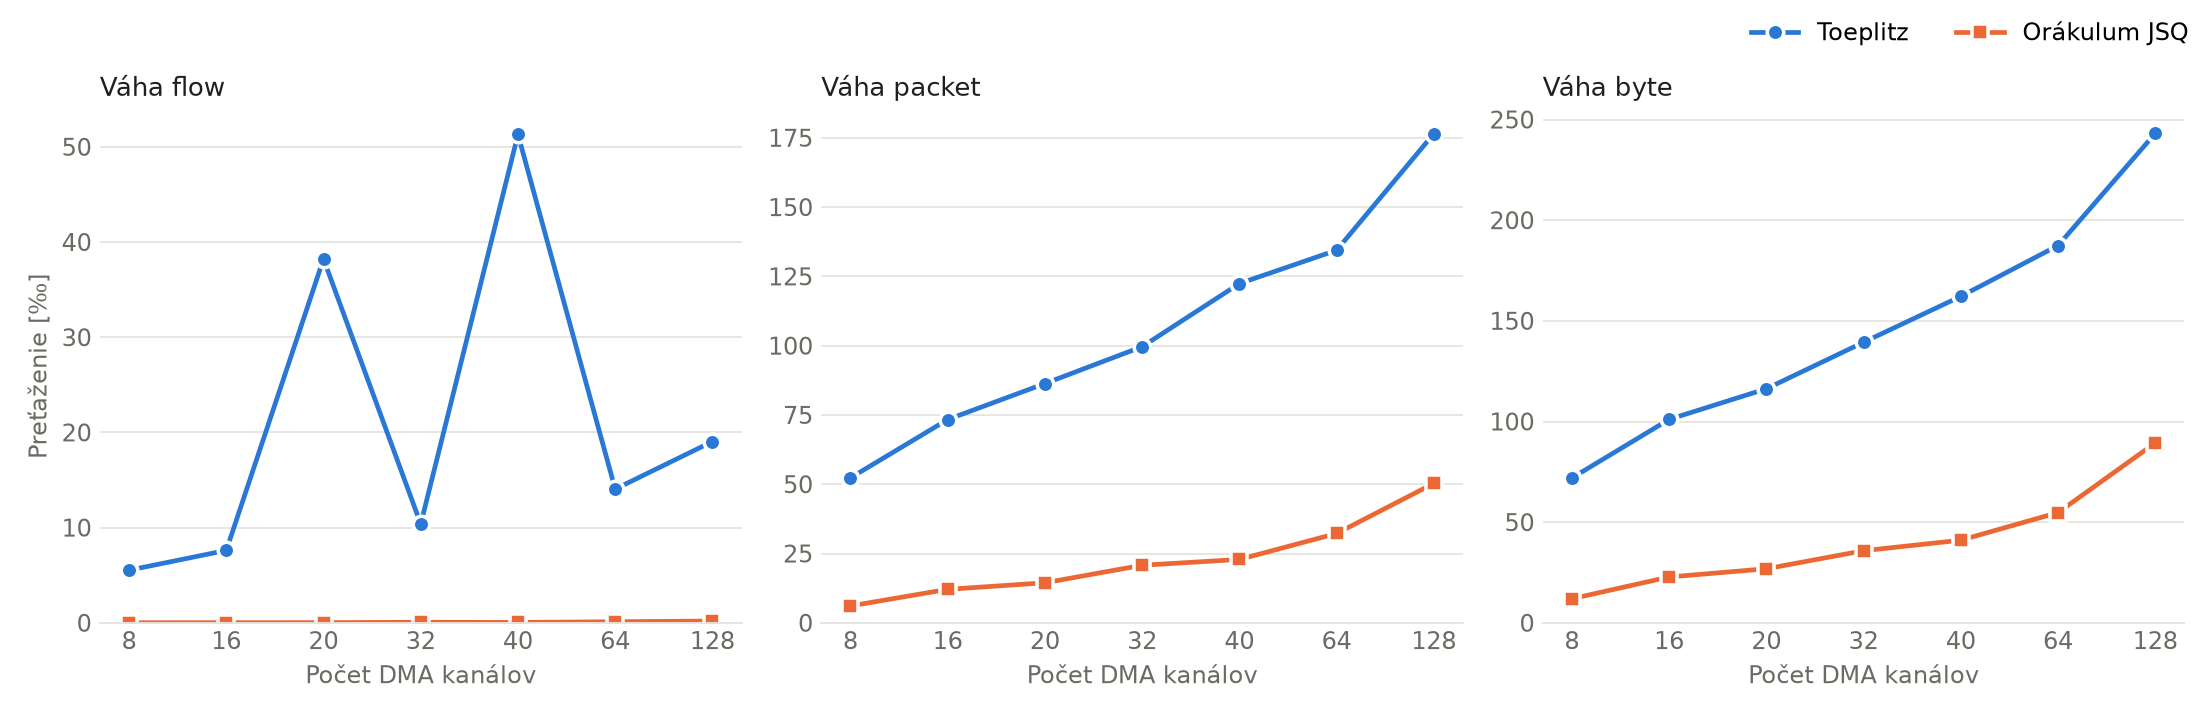
\includegraphics[width=\textwidth]{analyza/jsq_vs_toeplitz.png}
  \caption{Preťaženie Toeplitzu a orákula JSQ pri pevnom okne, \texttt{odid1}.}
  \label{fig:jsq}
\end{figure}

Orákulum JSQ (sekcia~\ref{sec:jsq}) stále posiela celý tok do jedného kanála, ale vyberá ho
podľa záťaže. Oproti Toeplitzu znižuje preťaženie o~71 až 88\,\% pri váhe \texttt{packet}
a o~63 až 83\,\% pri váhe \texttt{byte} (tabuľka~\ref{tab:jsq}). Pri 128 kanáloch stúpne
Jainov index z~0,774 na 0,949 (packet) a z~0,645 na 0,893 (byte).

Z~toho vyplývajú dva závery:

\begin{enumerate}
  \item \textbf{Veľká rezerva je v~politike výberu kanála, nie v~hashi.} Funkcie sa líšia
        o~jednotky percent, lepšie priradenie tokov dokáže odstrániť väčšinu preťaženia.
  \item \textbf{Zvyšok je cena afinity.} Aj orákulum má pri 128 kanáloch
        50,3\,\textperthousand{} (packet) a 89,4\,\textperthousand{} (byte). Toto preťaženie
        sa pri pravidle ,,jeden tok = jeden kanál`` už znižuje ťažko, čo motivuje varianty
        rozdeľujúce tok na viac kanálov.
\end{enumerate}

\emph{Obmedzenia:} orákulum pozná budúcnosť toku, takže ide o~dolnú hranicu, nie realizovateľný
návrh. Nepoužíva RETA, preto časť jeho výhody pri 20 a 40 kanáloch tvorí iba chýbajúca kvantizácia.

\section{Vplyv veľkosti okna}
\label{sec:vplyv-okna}

% !TEX root = ../projekt.tex
\begin{table}[ht]
  \centering
  \small
  \caption{Pevné okno (150\,000 paketov) a dynamické okno (18\,750 paketov na kanál), váha packet, \texttt{odid1}. Hodnoty sú preťaženie v \textperthousand.}
  \label{tab:dynamicke-okno}
  \begin{tabular}{r r r rr rr r}
    \toprule
    & & & \multicolumn{2}{c}{Toeplitz} & \multicolumn{2}{c}{JSQ} & JSQ oproti \\
    Kanály & Okno & Okien & pevné & dyn. & pevné & dyn. & Toeplitzu (dyn.) \\
    \midrule
    8 & 150\,000 & 15\,190 & 52,3 & 52,3 & 6,1 & 6,1 & $-88$\,\% \\
    16 & 300\,000 & 7\,595 & 73,3 & 73,1 & 12,1 & 12,5 & $-83$\,\% \\
    20 & 375\,000 & 6\,076 & 86,3 & 86,0 & 14,4 & 12,5 & $-85$\,\% \\
    32 & 600\,000 & 3\,797 & 99,6 & 98,9 & 20,8 & 18,9 & $-81$\,\% \\
    40 & 750\,000 & 3\,038 & 122,4 & 121,5 & 22,9 & 21,3 & $-82$\,\% \\
    64 & 1\,200\,000 & 1\,898 & 134,4 & 132,6 & 32,2 & 28,5 & $-79$\,\% \\
    128 & 2\,400\,000 & 949 & 176,5 & 172,9 & 50,3 & 45,0 & $-74$\,\% \\
    \bottomrule
  \end{tabular}
\end{table}


\begin{figure}[ht]
  \centering
  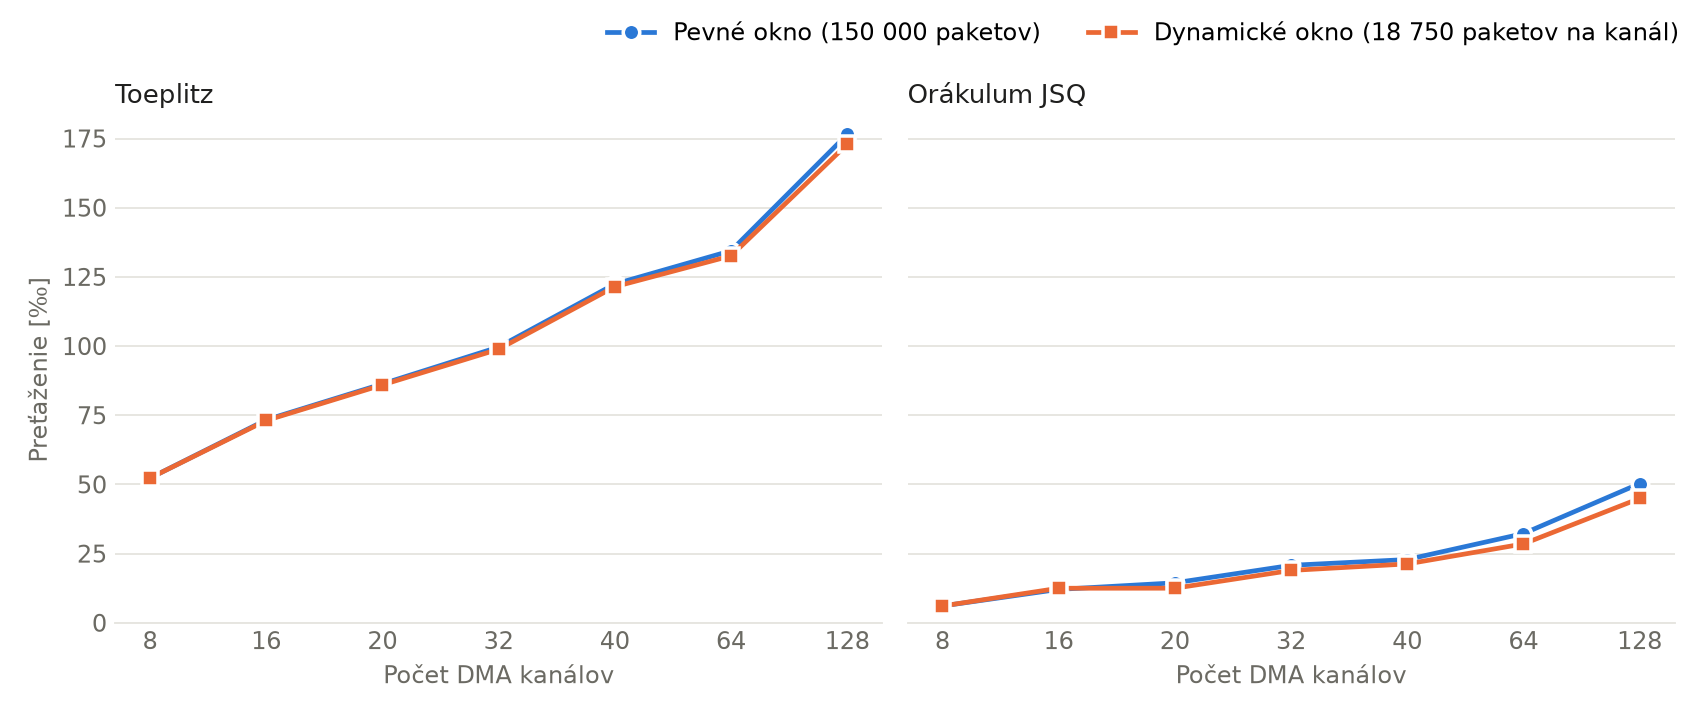
\includegraphics[width=0.9\textwidth]{analyza/pevne_vs_dynamicke_okno.png}
  \caption{Pevné a dynamické okno, váha packet, \texttt{odid1}.}
  \label{fig:okno}
\end{figure}

Pri pevnom okne dostane jeden kanál pri 128 kanáloch 16-krát menej paketov než pri 8.
Mohlo by sa preto zdať, že rast preťaženia s~počtom kanálov je iba artefakt merania.
Tabuľka~\ref{tab:dynamicke-okno} ukazuje, že na \texttt{odid1} to tak \textbf{nie je}: pri
128 kanáloch klesne preťaženie Toeplitzu po prechode na dynamické okno iba zo 176,5 na
172,9\,\textperthousand{} (približne 2\,\%) a orákula z~50,3 na 45,0\,\textperthousand.
Rast preťaženia je teda vlastnosťou prevádzky, nie dĺžky okna.

\emph{Poznámka:} na malom syntetickom datasete (\texttt{flow\_big}, približne 883 súbežných
smerov tokov) bol vplyv okna oveľa väčší (662 oproti 391\,\textperthousand). Výsledok preto
závisí od počtu súbežných tokov a treba ho overiť na ďalších vzorkách.

\section{Ďalšie vzorky prevádzky}
\label{sec:dalsie-vzorky}

Porovnanie funkcií prebehlo aj na vzorkách \texttt{odid2}, \texttt{odid4} a \texttt{odid6} a na
\texttt{odid1} s~hashovaním iba IP adries. Všetky grafy sú v~prílohe~\ref{app:grafy}.

\textbf{Pozor na rozdiely oproti predošlým sekciám:} tieto behy pochádzajú zo staršej verzie
kódu a namiesto jednoduchej tabelácie obsahujú multiply-shift (NH). Surové výsledky sa neuložili,
preto sú čísla v~tabuľke~\ref{tab:vzorky} iba \emph{orientačne odčítané z~grafov}.
\TODO{Prepočítať novým simulátorom a nahradiť presnými hodnotami.}

\begin{table}[ht]
  \centering
  \small
  \caption{Toeplitz na rôznych vzorkách, váha \texttt{packet}, bez symetrie, pevné okno.
  Okrem \texttt{odid1} (plný tuple) sú hodnoty orientačne odčítané z~grafov.}
  \label{tab:vzorky}
  \begin{tabular}{l r r l}
    \toprule
    Vzorka & 8 kanálov [\textperthousand] & 128 kanálov [\textperthousand] & Najväčšia odchýlka funkcie od Toeplitzu \\
    \midrule
    \texttt{odid1} (plný tuple) & 52   & 177  & 7\,\% (Chaskey, lepší) \\
    \texttt{odid2}              & 70   & 240  & 7,5\,\% (multiply-shift, horší) \\
    \texttt{odid4}              & 185  & 525  & 1,6\,\% (multiply-shift, lepší) \\
    \texttt{odid6}              & 115  & 280  & 1,3\,\% \\
    \texttt{odid1} (iba IP)     & 65   & 220  & 12\,\% (multiply-shift, horší) \\
    \bottomrule
  \end{tabular}
\end{table}

Z~porovnania vzoriek vyplývajú tri pozorovania:

\begin{enumerate}
  \item \textbf{Úroveň preťaženia závisí od prevádzky.} Medzi vzorkami sa líši približne
        3,5-násobne (pri 8 kanáloch 52 až 185\,\textperthousand). Rast s~počtom kanálov majú
        všetky vzorky.
  \item \textbf{Kvalitné funkcie zostávajú blízko seba.} Toeplitz, jhash, Chaskey a HalfSipHash
        sa pri váhe \texttt{packet} líšia najviac o~jednotky percent na každej vzorke.
  \item \textbf{Slabšia funkcia sa môže prejaviť pri vstupe s~nízkou entropiou.} Pri hashovaní iba IP
        adries je multiply-shift horší než Toeplitz konzistentne pri všetkých počtoch kanálov:
        približne o~6--12\,\% (packet), 6--11\,\% (byte) a 4--16\,\% (flow). Menší náznak je aj
        na \texttt{odid2} (do 7,5\,\%). Výber hashu teda nie je úplne ľubovoľný.
        \TODO{Príčinu (nízka entropia vstupu) sme zatiaľ neoverili, je to hypotéza.}
\end{enumerate}

\begin{figure}[ht]
  \centering
  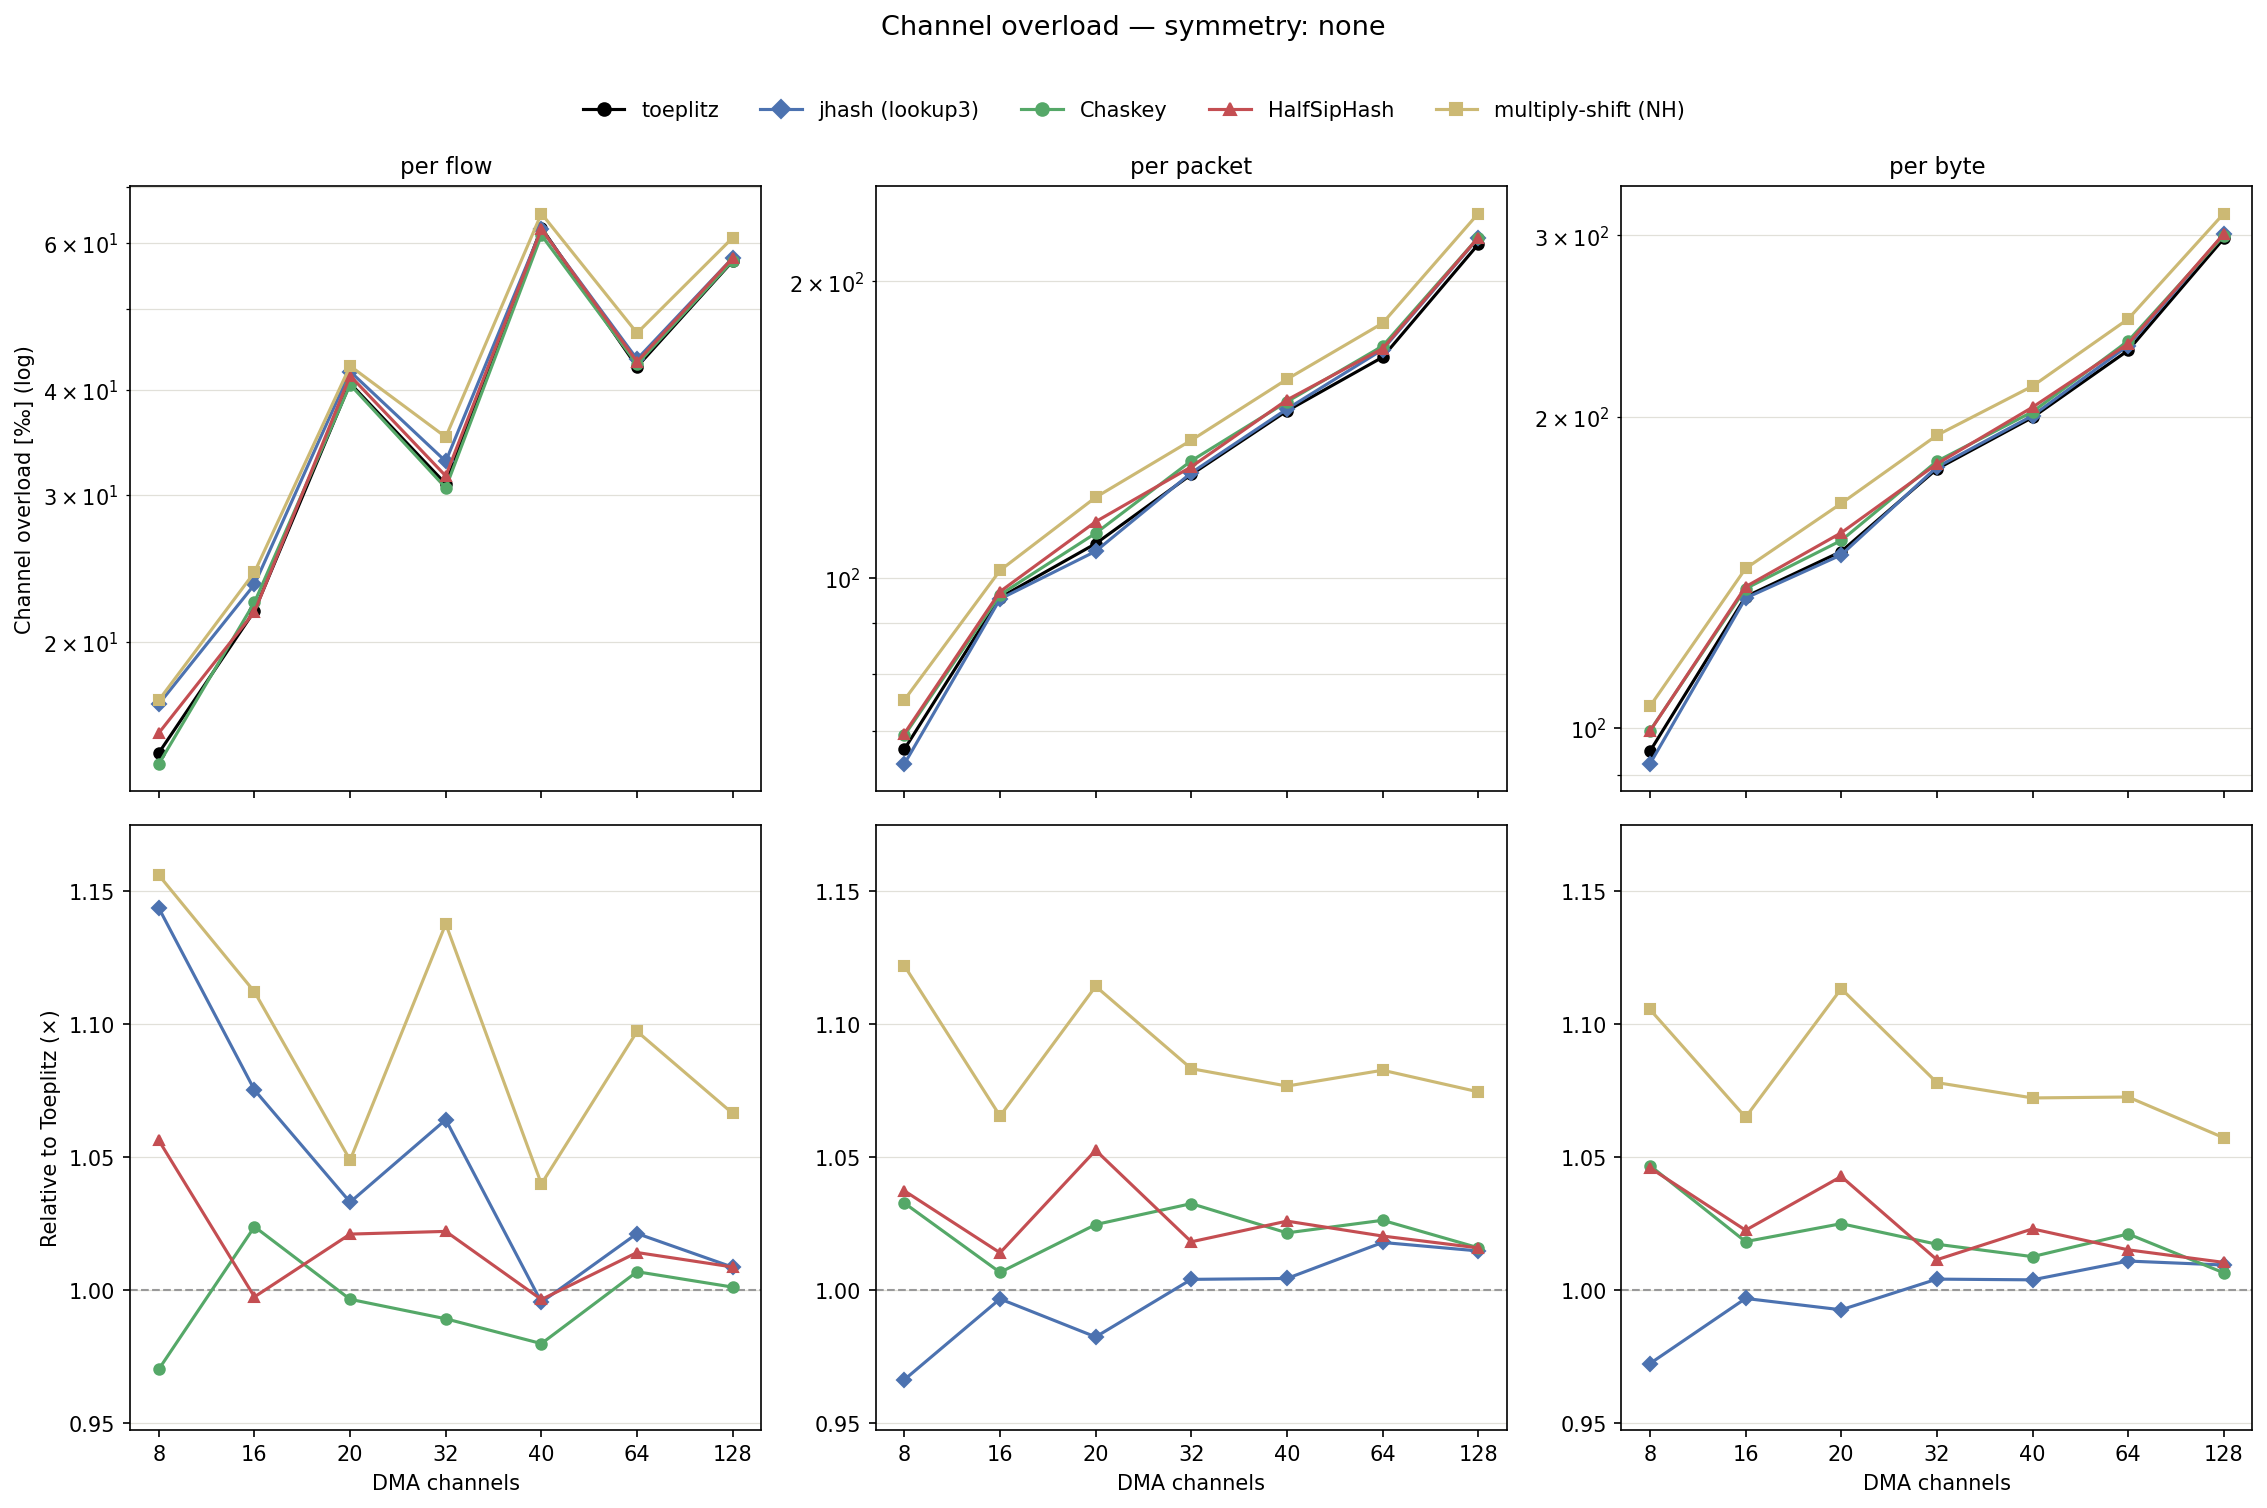
\includegraphics[width=\textwidth]{ostatne_vzorky/odid1_ip_only/overload_none.png}
  \caption{Hashovanie iba IP adries, \texttt{odid1}, staršia verzia kódu s~funkciou multiply-shift.
  V~spodnom riadku je vidno, že multiply-shift je pri všetkých váhach nad Toeplitzom.}
  \label{fig:ip-only}
\end{figure}

Hashovanie iba IP adries navyše zvyšuje samotné preťaženie: pri 128 kanáloch a váhe \texttt{flow}
je približne 57\,\textperthousand{} oproti 19,0\,\textperthousand{} pri plnom tuple
(obrázok~\ref{fig:ip-only}), lebo všetky toky medzi tou istou dvojicou adries skončia v~jednom kanáli.

\section{Zhrnutie}

\begin{enumerate}
  \item Nerovnomernú záťaž spôsobuje rozdielna veľkosť tokov, nie kvalita hashu.
  \item Medzi kvalitnými hashmi sa nepreukázal rozdiel väčší než vplyv kľúča. Slabá funkcia
        (multiply-shift) však môže byť horšia pri vstupe s~nízkou entropiou.
  \item Kľúč má pri malom počte kanálov veľký vplyv: pri 8 kanáloch 42 až 71\,\textperthousand.
  \item Symetria stojí 14--18\,\% pri váhach flow a packet, 2--4\,\% pri bajtoch.
  \item Pri počtoch kanálov, ktoré nedelia 128, pridáva preťaženie aj tabuľka RETA.
  \item Lepší výber kanála pri zachovaní afinity by mohol odstrániť 63--88\,\% preťaženia.
  \item Dĺžka okna výsledky na \texttt{odid1} takmer nemení.
\end{enumerate}

  % !TEX root = ../projekt.tex
% =============================================================================
% STAV: návrhy a nápady (bod 4 zadania). Implementované je iba to, čo je
% v tabuľke označené. Ostatné je plán, nie výsledok.
% =============================================================================
\chapter{Návrh variantov jednotky RSS}
\label{chap:varianty}

Analýza ukázala, že hash nie je úzkym miestom. Varianty sa preto zameriavajú na to,
\emph{ako sa z~hashu alebo zo stavu kanálov určí kanál}. Podľa zadania sa delia do dvoch skupín.

\begin{table}[ht]
  \centering
  \small
  \caption{Prehľad variantov a ich aktuálny stav.}
  \label{tab:varianty}
  \begin{tabular}{l l l}
    \toprule
    Varianta & Afinita toku & Stav \\
    \midrule
    A1 Iná hashovacia funkcia     & áno & vyhodnotené, bez prínosu \\
    A2 Symetria                   & áno & vyhodnotené, má cenu \\
    A3 Väčšia RETA                & áno & návrh \\
    A4 Úprava hashu (digest)      & áno & návrh \\
    A5 RETA podľa záťaže          & áno & návrh \\
    A6 Orákulum JSQ               & áno & hotové, dolná hranica \\
    \midrule
    B1 Skupiny susedných kanálov  & nie & návrh \\
    B2 Flowlety                   & nie & návrh \\
    B3 Dva hashe a výber v~podmnožine & nie & návrh \\
    B4 Rozdelenie iba veľkých tokov & nie & návrh \\
    \bottomrule
  \end{tabular}
\end{table}

\section{Varianty so zachovaním afinity toku}

\subsection*{A1: Iná hashovacia funkcia}
Vyhodnotené v~sekciách~\ref{sec:hash-nezalezi} až~\ref{sec:statistika}. Medzi kvalitnými funkciami
sa prínos nepreukázal. Slabšia funkcia môže pri vstupe s~nízkou entropiou výsledok zhoršiť
(sekcia~\ref{sec:dalsie-vzorky}).

\subsection*{A2: Symetria}
Vyhodnotené v~sekcii~\ref{sec:cena-symetrie}. Je to funkčná požiadavka s~merateľnou cenou,
nie optimalizácia.

\subsection*{A3: Väčšia tabuľka RETA}
Odstraňuje kvantizáciu pri počtoch kanálov, ktoré nedelia veľkosť tabuľky. Pri 512 položkách
klesne teoretické preťaženie dokonalého hashu z~37,5 na 9,4\,\textperthousand{} ($n=20$)
a z~50,0 na 12,5\,\textperthousand{} ($n=40$). \TODO{Zistiť cenu v~pamäti FPGA.}

\subsection*{A4: Úprava hashu pred výberom položky}
Medzi hash a RETA sa vloží lacná operácia, napríklad zmiešanie horných bitov do spodných
($h \oplus (h \gg 16)$). \emph{Očakávanie:} vzhľadom na výsledky A1 skôr malý prínos, je to však
najlacnejšia zmena.

\subsection*{A5: Plnenie RETA podľa záťaže}
Položky RETA sa medzi oknami presúvajú z~preťažených kanálov na menej zaťažené. Hardvér meria
záťaž položiek a tabuľku preprogramuje. Je to realizovateľná aproximácia orákula.
\TODO{Otvorené: ako často meniť tabuľku a čo s~tokmi, ktoré sa pri zmene presunú
(krátkodobé preusporiadanie paketov).}

\emph{Dopad na simulátor:} kanál sa dnes určí raz pri štarte toku. Pre A5 sa musí pre tok uložiť
položka RETA a kanál určovať až pri skladaní okna.

\subsection*{A6: Orákulum JSQ}
Popísané v~sekcii~\ref{sec:jsq}. Nie je to návrh pre hardvér, ale referencia, s~ktorou sa
porovnávajú ostatné varianty.

\section{Varianty rozdeľujúce tok na podmnožinu kanálov}

Tieto varianty útočia priamo na príčinu z~sekcie~\ref{sec:slony}: veľký tok už nemusí celý
zaťažiť jeden kanál. \textbf{Cenou je možné preusporiadanie paketov toku}, preto k~nim treba
pridať novú metriku. \TODO{Navrhnúť metriku preusporiadania a overiť s~vedúcim, koľko kanálov
v~skupine je prijateľných pre aplikácie.}

\subsection*{B1: Skupiny susedných kanálov}
Hash vyberie skupinu susedných kanálov a pakety toku sa v~nej striedajú (\emph{round robin}).
Pôvodný nápad: skupiny po 2 kanáloch pri 8 kanáloch a po 3 až 6 pri 128 kanáloch, lebo hardvér
vie susedné kanály prepojiť.

\subsection*{B2: Flowlety}
Tok sa rozdelí v~medzerách medzi paketmi väčších než zvolený prah a každá časť sa hashuje zvlášť.
\emph{Obmedzenie simulátora:} pakety sú v~toku rozložené rovnomerne, takže skutočné medzery
nevidí. Na túto variantu by bola potrebná paketová stopa. \TODO{Zvážiť, či ju vôbec zaradiť.}

\subsection*{B3: Dva hashe a výber v~podmnožine}
Hash určí podmnožinu $k$ kanálov a v~nej sa pre paket vyberie kanál druhým mechanizmom:
striedaním, druhým hashom alebo podľa najmenšej záťaže.

\subsection*{B4: Rozdelenie iba veľkých tokov}
Malé toky zostávajú v~jednom kanáli, rozdelia sa iba toky, ktoré počas behu prekročia prah.
Väčšina tokov sa teda nepreusporiada a záťaž veľkých tokov sa rozloží.

\emph{Dopad na simulátor pre skupinu B:} kanál sa musí vyberať pre každý paket, nie raz pre tok.

\TODO{Vybrať 3--4 varianty, ktoré sa naozaj implementujú. Návrh: A3, A5, B1, B4.}

  % !TEX root = ../projekt.tex
% =============================================================================
% STAV: iba kostra, výsledky zatiaľ neexistujú (bod 5 zadania).
% =============================================================================
\chapter{Vyhodnotenie variantov}
\label{chap:vyhodnotenie}

\TODO{Kapitola sa dá napísať až po implementácii variantov z~kapitoly~\ref{chap:varianty}.}

\section{Nastavenie experimentov}
\TODO{Datasety, hash Toeplitz, 16 kľúčov, kanály 8--128, dynamické okno, váhy packet a byte.}

\section{Varianty so zachovaním afinity}
\TODO{Pre každú variantu: preťaženie a Jain oproti Toeplitzu a JSQ. Koľko z~rezervy medzi
Toeplitzom a orákulom varianta využije?}

\section{Varianty rozdeľujúce tok}
\TODO{Preťaženie, Jain a metrika preusporiadania. Vplyv veľkosti skupiny.}

\section{Porovnanie na viacerých vzorkách}
\TODO{Správajú sa varianty rovnako na všetkých datasetoch?}

\section{Diskusia a odporúčanie}
\TODO{Ktorý variant odporučiť pre NDK a pri akom počte kanálov. Odhad nákladov v~hardvéri.}

  % !TEX root = ../projekt.tex
% =============================================================================
% STAV: rozpracované, dopísať po vyhodnotení variantov (bod 6 zadania).
% =============================================================================
\chapter{Záver}
\label{chap:zaver}

Práca sa zaoberala distribúciou paketov do DMA kanálov jednotkou RSS frameworku NDK. Vznikol
simulátor jednotky RSS pre najviac 128 kanálov, ktorý pracuje so záznamami reálnej prevádzky
a záťaž hodnotí preťažením, Jainovým indexom a normalizovaným $\chi^2$.

Analýza vzorky \texttt{odid1} ukázala, že nerovnomernú záťaž nespôsobuje kvalita hashu, ale
rozdielna veľkosť tokov. Medzi piatimi hashovacími funkciami sa nepreukázal rozdiel väčší než
vplyv náhodného kľúča, slabšia funkcia sa však môže prejaviť pri vstupe s~nízkou entropiou. Referenčné orákulum, ktoré zachováva afinitu toku, znížilo preťaženie
oproti Toeplitzu o~63 až 88\,\% pri váhach packet a byte, čo ukazuje veľkú rezervu v~spôsobe
výberu kanála.

\TODO{Doplniť výsledky navrhnutých variantov a odporúčanie pre NDK.}

\paragraph{Možnosti pokračovania.}
\TODO{Napríklad implementácia najlepšej varianty vo VHDL, meranie na reálnom hardvéri,
vyhodnotenie na paketových stopách namiesto tokových záznamov.}


  % Použitá literatúra / Bibliography
  % ----------------------------------------------
\ifslovak
  \makeatletter
  \def\@openbib@code{\addcontentsline{toc}{chapter}{Literatúra}}
  \makeatother
  \bibliographystyle{bib-styles/Pysny/skplain}
\else
  \ifczech
    \makeatletter
    \def\@openbib@code{\addcontentsline{toc}{chapter}{Literatura}}
    \makeatother
    \bibliographystyle{bib-styles/Pysny/czplain}
  \else
    \makeatletter
    \def\@openbib@code{\addcontentsline{toc}{chapter}{Bibliography}}
    \makeatother
    \bibliographystyle{bib-styles/Pysny/enplain}
  \fi
\fi
  \begin{flushleft}
  \nocite{*} % TEMPORARY: lists all entries until the chapters have real citations
  \bibliography{literatura}
  \end{flushleft}

  % vynechanie strany v obojstrannom režime
  \iftwoside
    \cleardoublepage
  \fi

  % Prílohy / Appendices
  % ---------------------------------------------
  \appendix
\ifczech
  \renewcommand{\appendixpagename}{Přílohy}
  \renewcommand{\appendixtocname}{Přílohy}
  \renewcommand{\appendixname}{Příloha}
\fi
\ifslovak
  \renewcommand{\appendixpagename}{Prílohy}
  \renewcommand{\appendixtocname}{Prílohy}
  \renewcommand{\appendixname}{Príloha}
\fi

  \startcontents[chapters]
  \setlength{\parskip}{0pt}

  \ifODSAZ
    \setlength{\parskip}{0.5\bigskipamount}
  \else
    \setlength{\parskip}{0pt}
  \fi

  \iftwoside
    \cleardoublepage
  \fi

  % !TEX root = ../projekt.tex
% =====================================================================
%  PRÍLOHA A — OBSAH PAMÄŤOVÉHO MÉDIA
% =====================================================================
\chapter{Obsah priloženého pamäťového média}
\label{app:medium}

\rozsah{0,5--1 strana. Povinná príloha — over si aktuálne požiadavky
fakulty na štruktúru odovzdávaného archívu.}

\pokyn{Vypíš stromovú štruktúru archívu a pri každom adresári jednu vetu,
čo obsahuje. Odporúčaná štruktúra:}

\begin{verbatim}
/
|-- text/        zdrojove subory prace (LaTeX) a vysledne PDF
|-- src/         evaluacny nastroj (zdrojove kody, requirements)
|-- rtl/         VHDL zdrojove kody rozsirenej RSS komponenty
|-- data/        vzorka vstupnych dat (alebo odkaz, ak sa nesmu zverejnit)
|-- results/     vysledne CSV subory a vygenerovane grafy
|-- scripts/     skripty na zopakovanie experimentov
`-- README.md    navod na spustenie
\end{verbatim}

\pozor{Pred odovzdaním uprac repozitár:
\begin{itemize}
  \item \texttt{README.md} je zastaraný (37\,B tuple, 64\,B kľúč, staré
        stĺpce a staré algoritmy) — musí zodpovedať finálnemu stavu,
  \item zmaž zvyšky \texttt{results/t.csv} a \texttt{resultsoverload\_comparison.png},
  \item \texttt{run.sh} odkazuje na neexistujúci \texttt{data/odid1.csv},
  \item \texttt{analyze.py:191} má pokazený nadpis grafu,
  \item oprav preklep \texttt{thresshold\_sum} $\rightarrow$ \texttt{threshold\_sum}.
\end{itemize}
Oponent si archív otvorí a skúsi spustiť \texttt{run.sh}. Ak to spadne
na prvom riadku, poznačí si to.}

\pokyn{Ak sa dáta CESNET nesmú zverejniť, napíš to sem explicitne a priloži
aspoň malú anonymizovanú vzorku alebo generátor syntetických dát, aby sa
nástroj dal spustiť aj bez nich.}

  % !TEX root = ../projekt.tex
% =============================================================================
% STAV: všetky doplnkové grafy z porovnania hashov (staršia verzia kódu, thesis_results/).
% =============================================================================
\chapter{Doplnkové grafy porovnania hashovacích funkcií}
\label{app:grafy}

Príloha obsahuje grafy ďalších vzoriek prevádzky. Pochádzajú zo staršej verzie simulátora: používajú 128 položiek RETA, 16 kľúčov, pevné okno 150\,000 paketov a namiesto jednoduchej tabelácie funkciu multiply-shift (NH). Grafy pre \texttt{odid1} s~plným tuple a aktuálnou sadou funkcií sú v~kapitole~\ref{chap:analyza}.

\TODO{Prekresliť so slovenskými popismi po prepočítaní novým simulátorom.}

\clearpage
\begin{figure}[p]
  \centering
  \begin{subfigure}{0.60\textwidth}
    \centering
    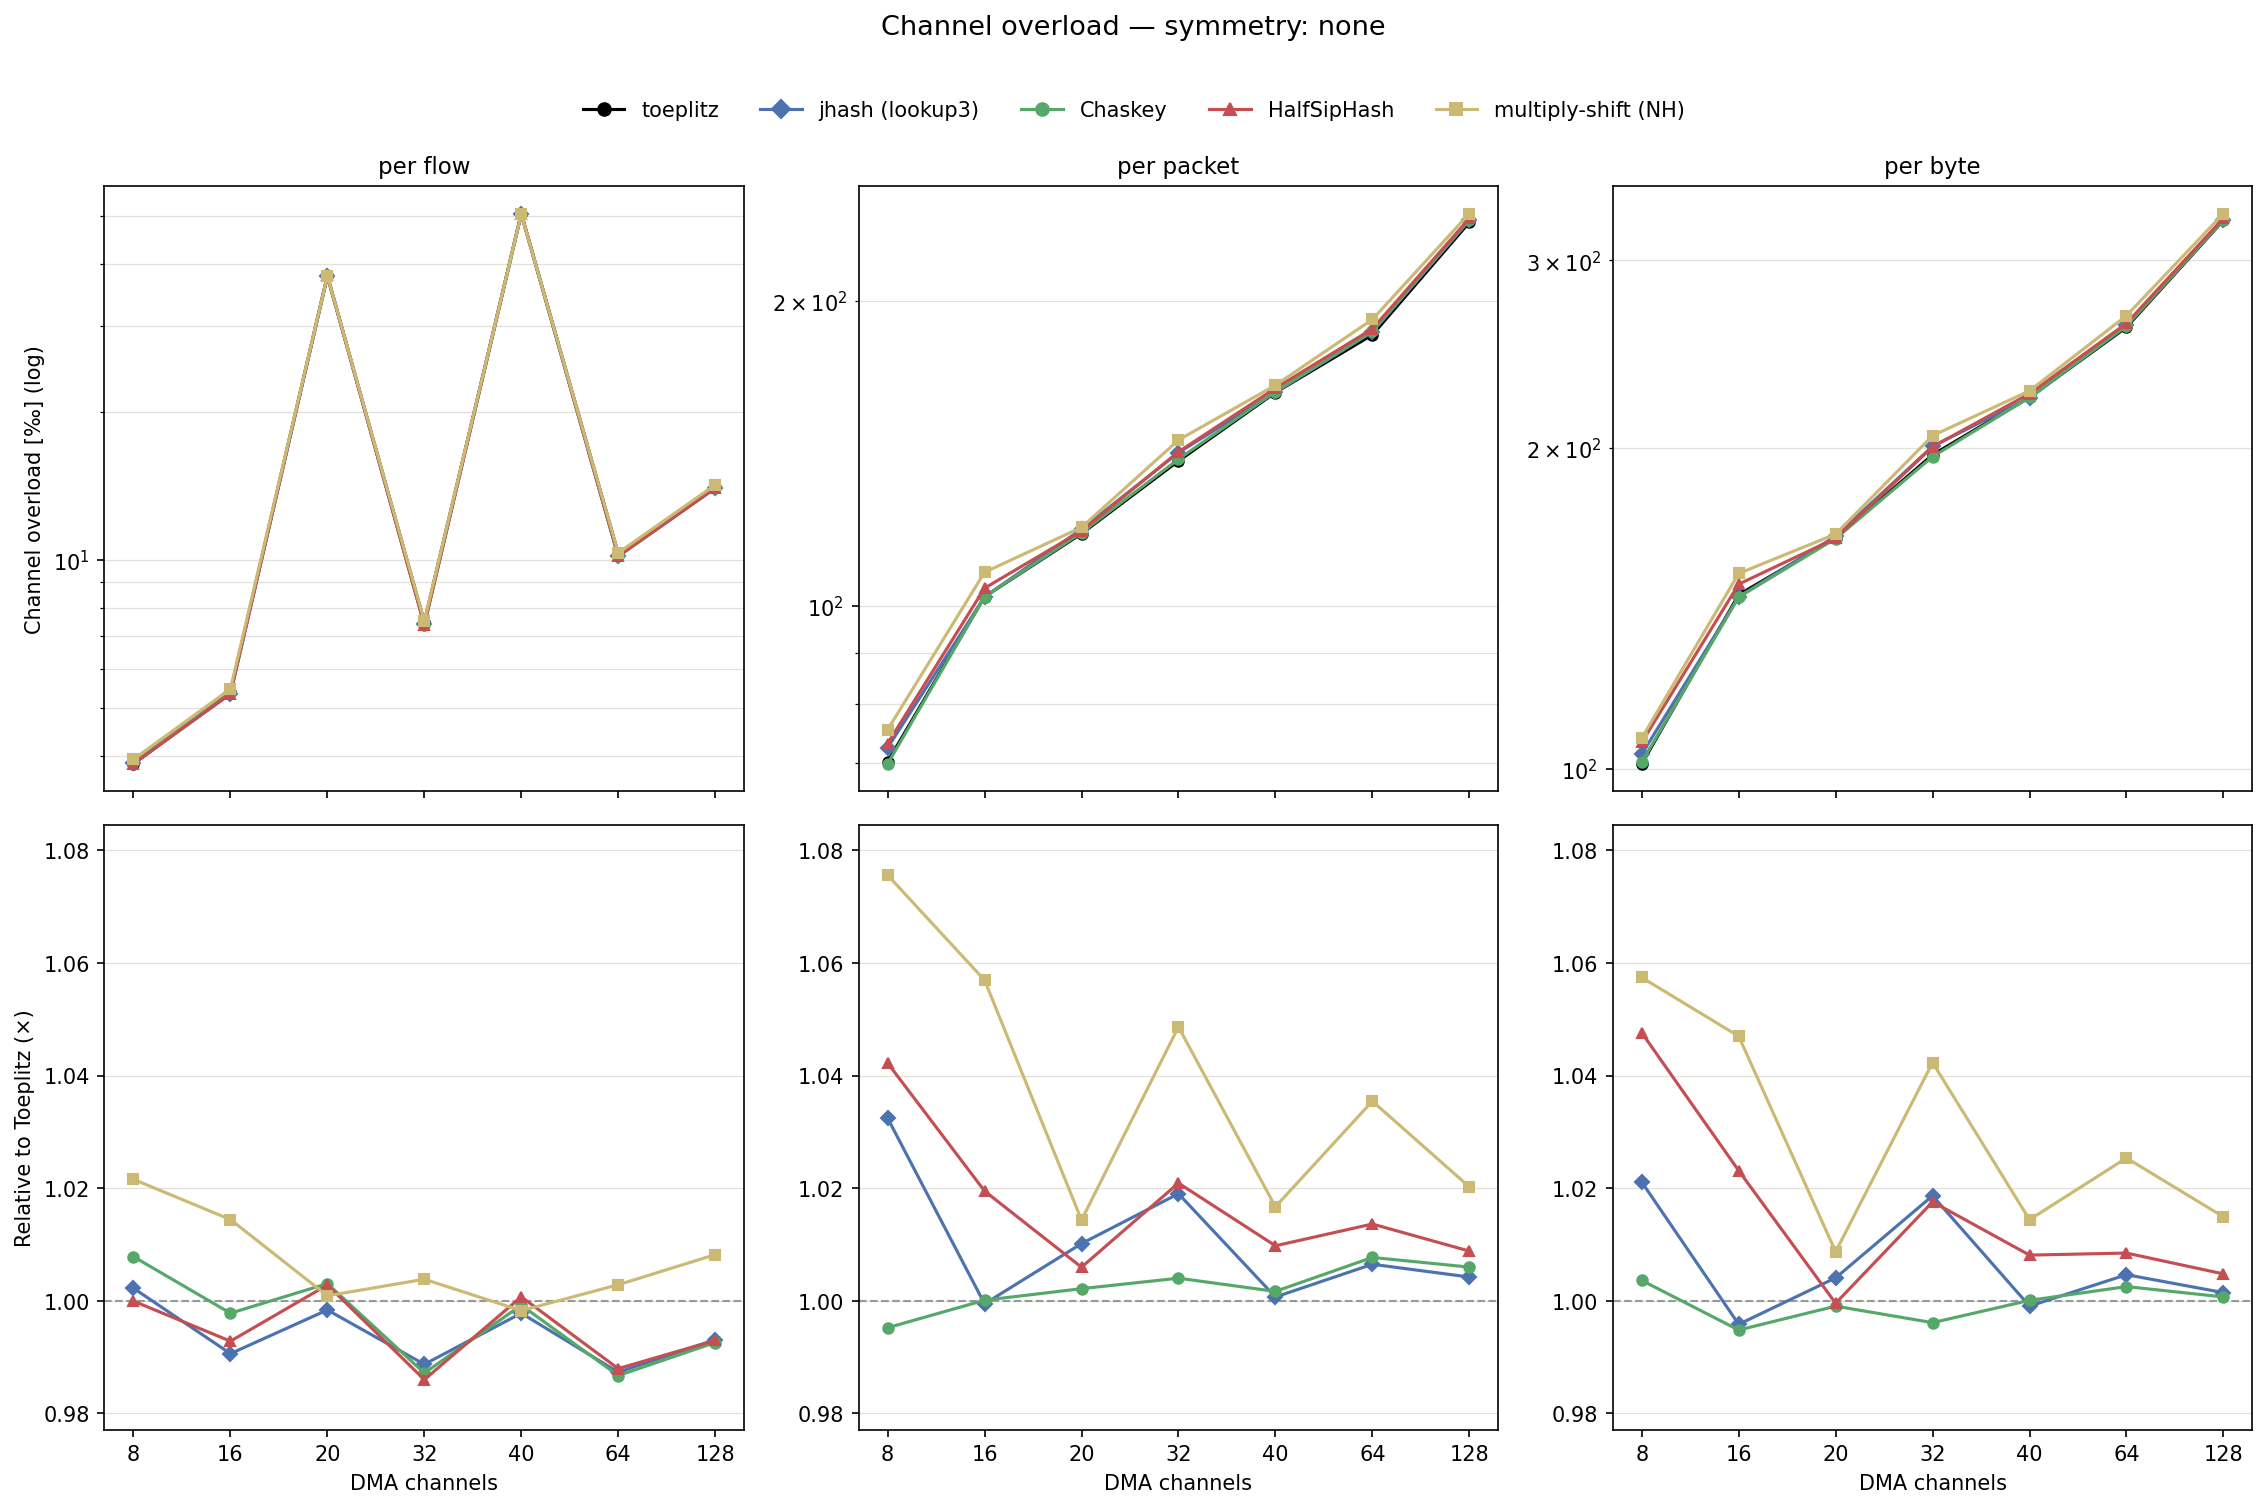
\includegraphics[width=\textwidth]{ostatne_vzorky/odid2_full_tuple/overload_none.png}
    \caption{bez symetrie}
  \end{subfigure}

  \begin{subfigure}{0.60\textwidth}
    \centering
    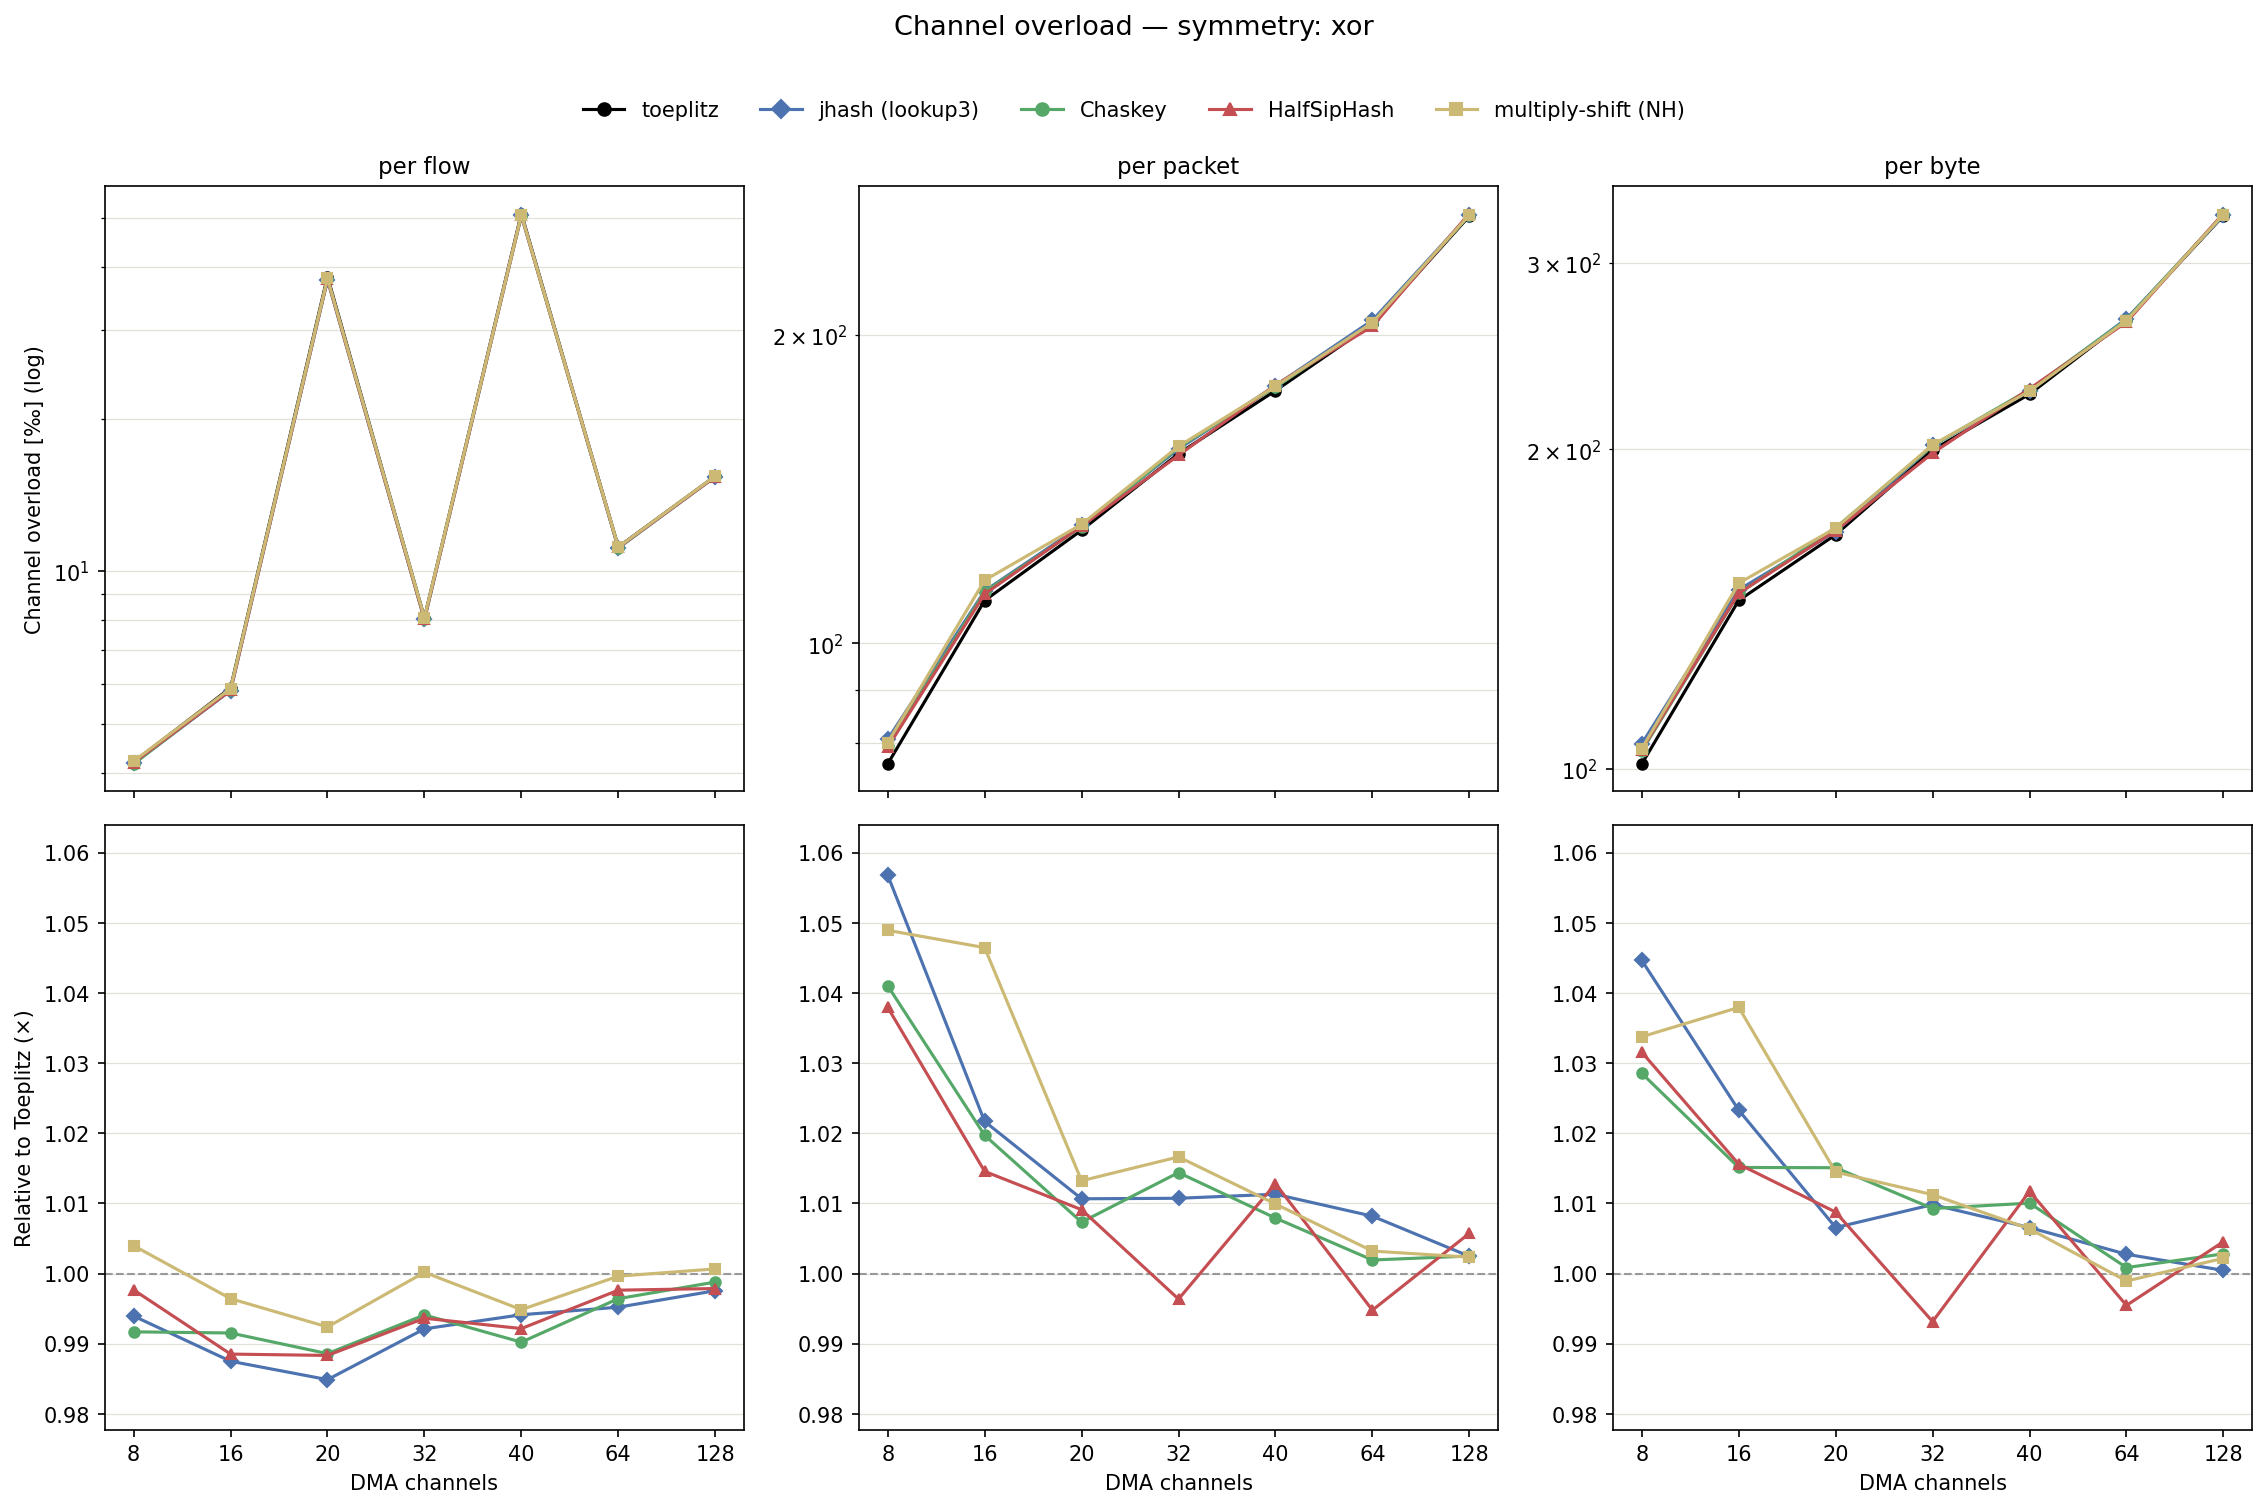
\includegraphics[width=\textwidth]{ostatne_vzorky/odid2_full_tuple/overload_xorfold.png}
    \caption{symetria XOR}
  \end{subfigure}

  \begin{subfigure}{0.60\textwidth}
    \centering
    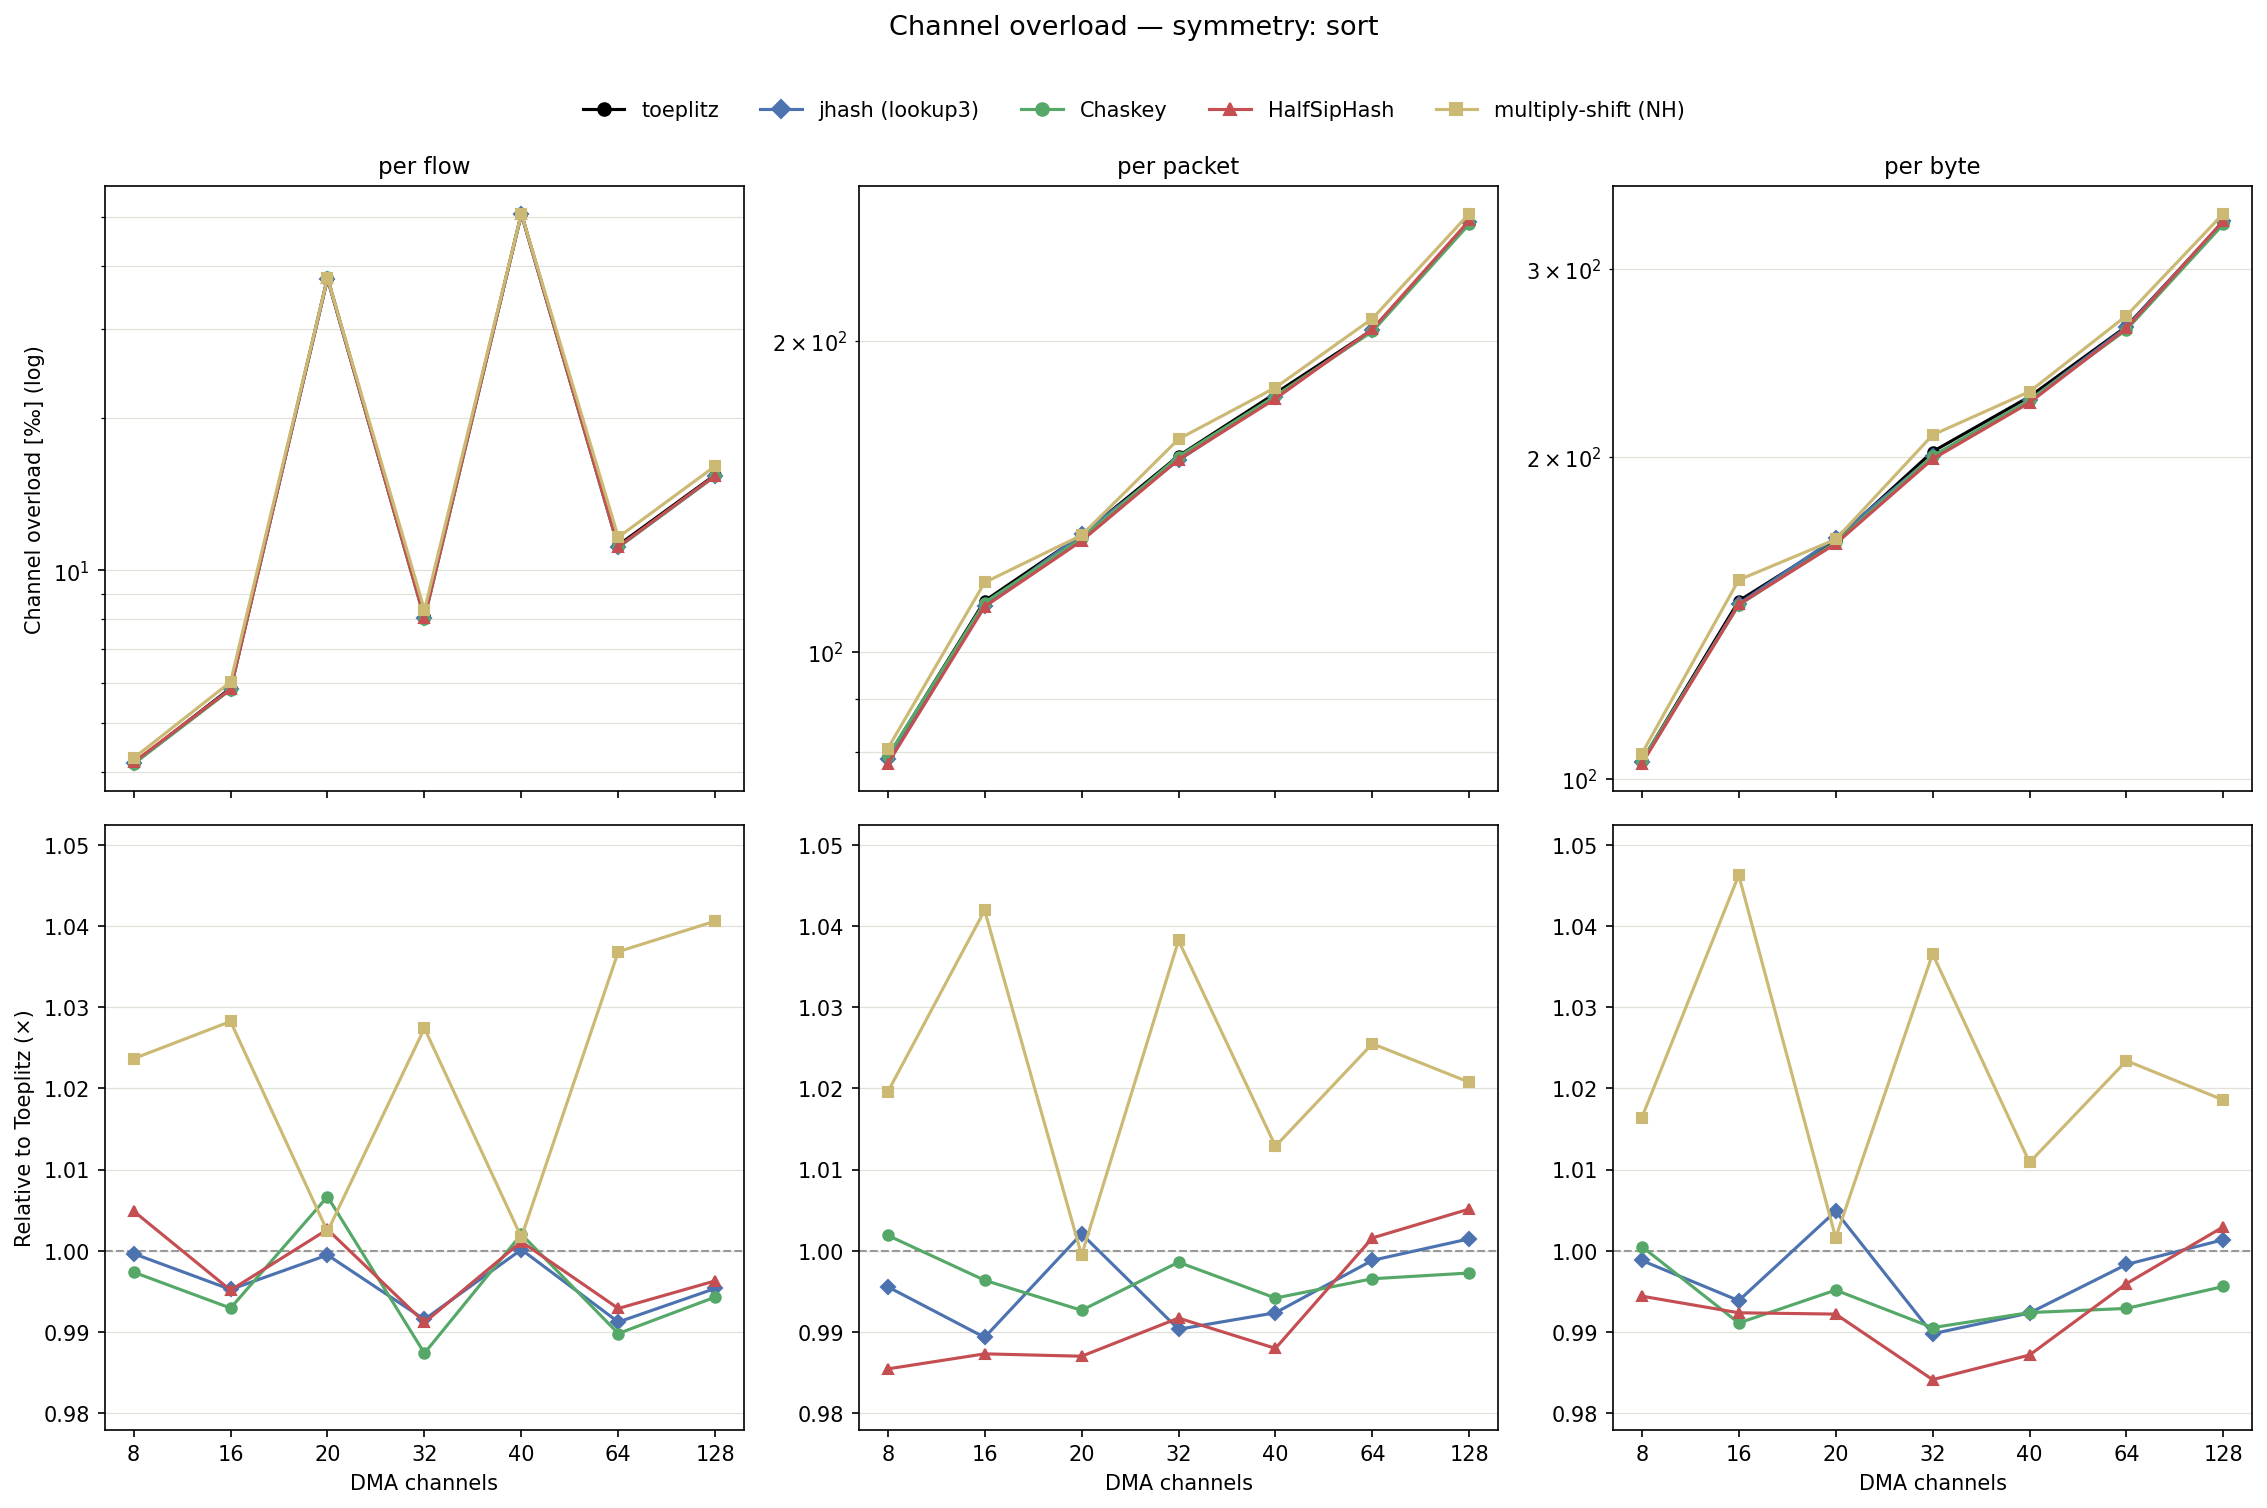
\includegraphics[width=\textwidth]{ostatne_vzorky/odid2_full_tuple/overload_sortfold.png}
    \caption{symetria sort}
  \end{subfigure}

  \caption{Preťaženie funkcií a pomer k~Toeplitzu: \texttt{odid2}, plný tuple.}
  \label{fig:b-odid2-full-tuple-overload}
\end{figure}

\begin{figure}[p]
  \centering
  \begin{subfigure}{0.54\textwidth}
    \centering
    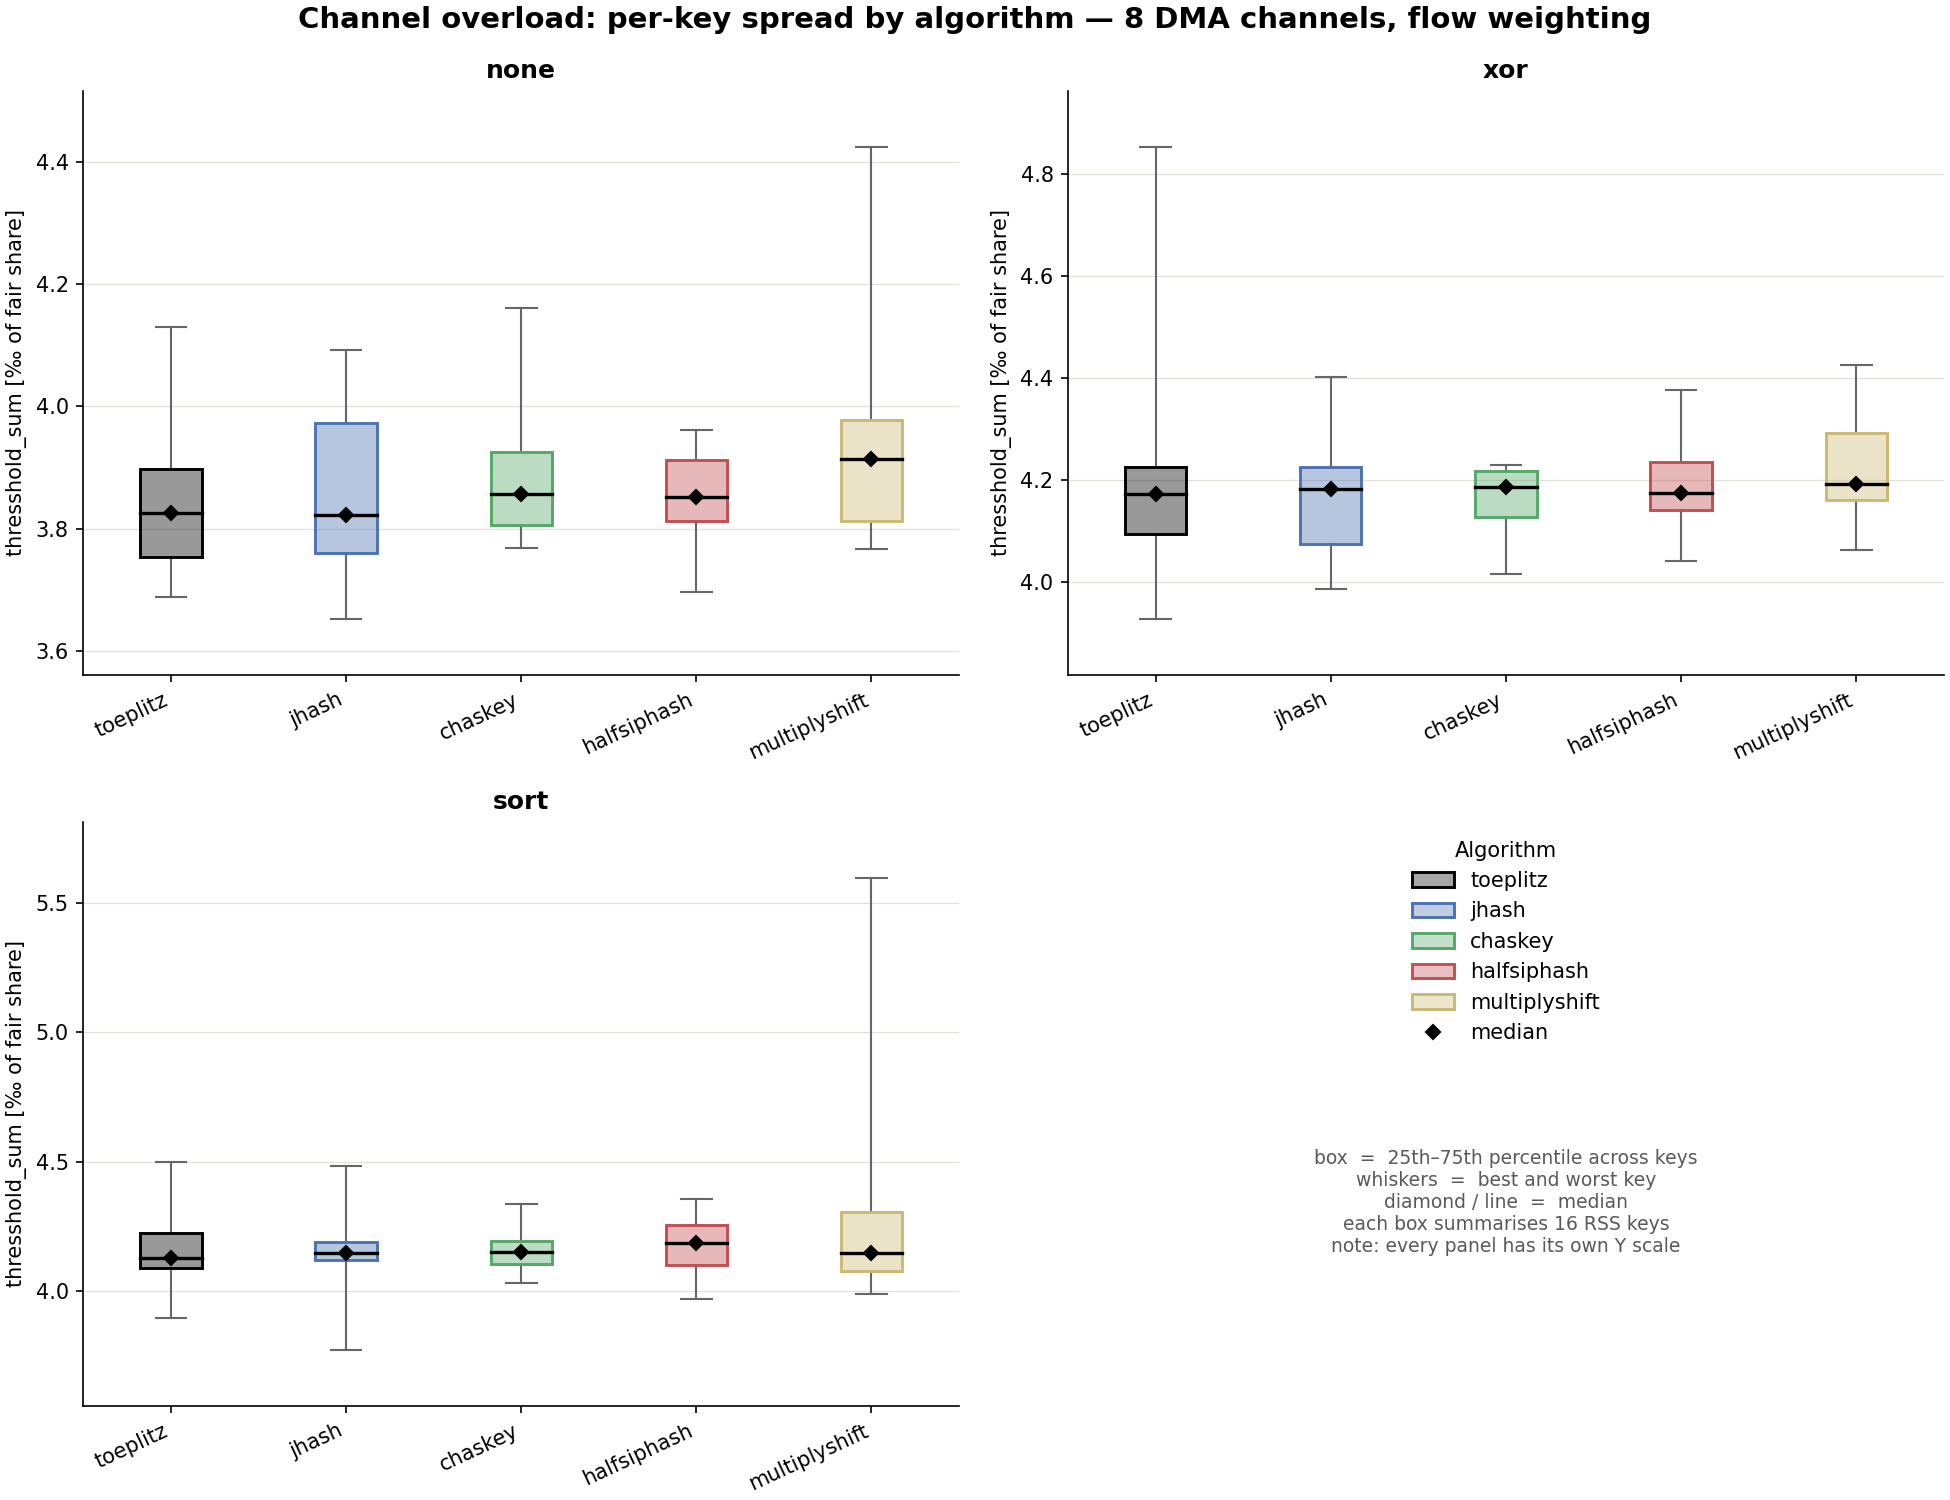
\includegraphics[width=\textwidth]{ostatne_vzorky/odid2_full_tuple/keys_8.png}
    \caption{8 kanálov}
  \end{subfigure}

  \begin{subfigure}{0.54\textwidth}
    \centering
    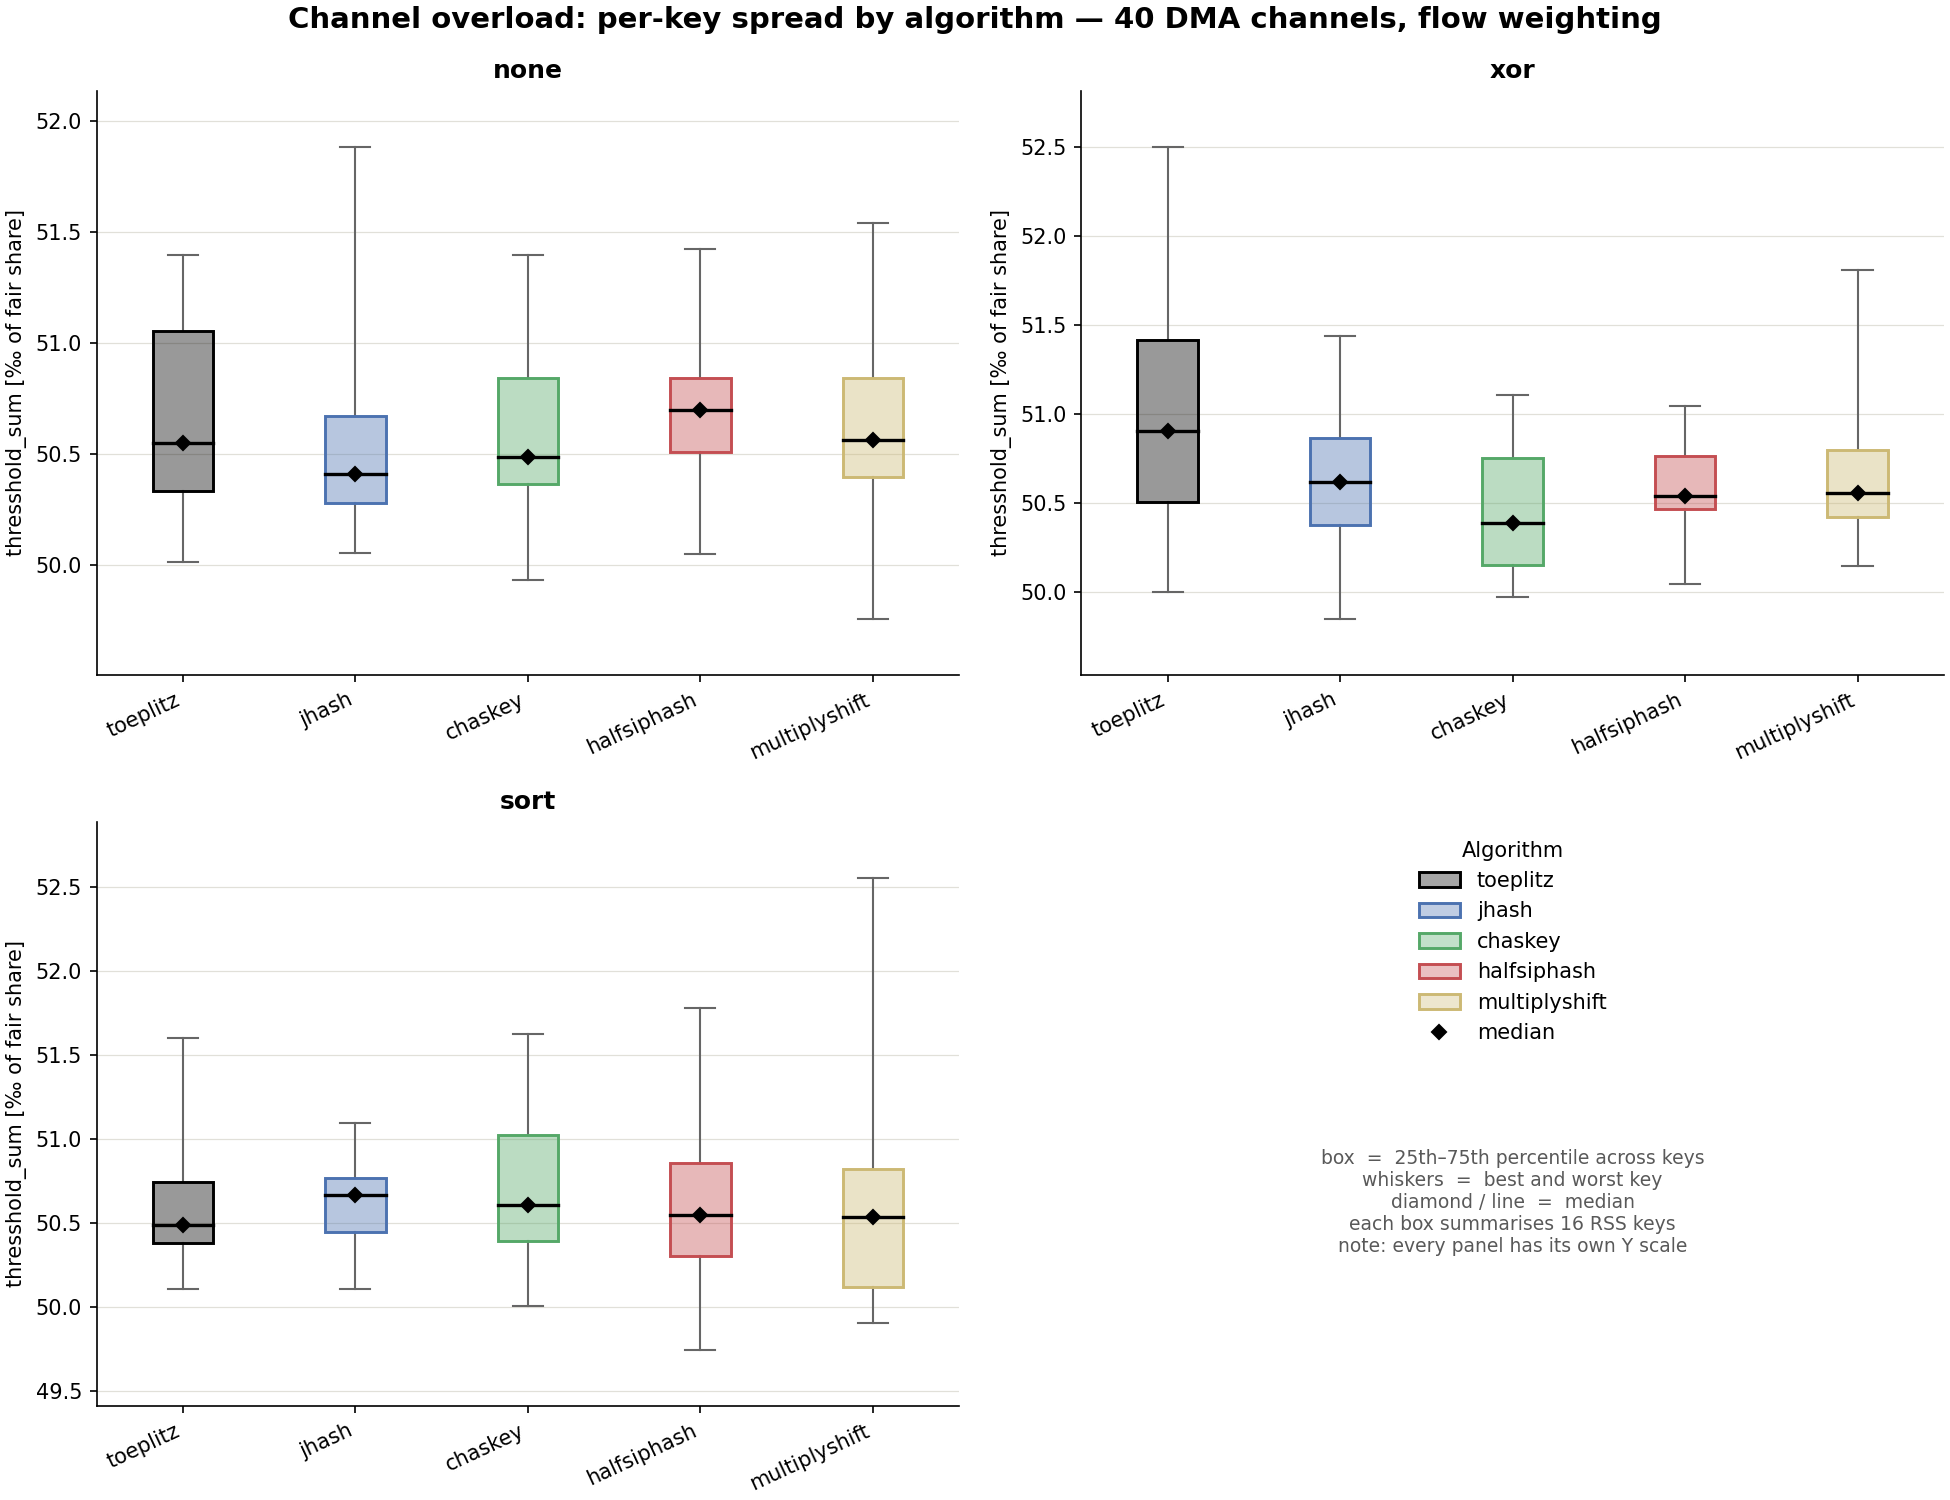
\includegraphics[width=\textwidth]{ostatne_vzorky/odid2_full_tuple/keys_40.png}
    \caption{40 kanálov}
  \end{subfigure}

  \begin{subfigure}{0.54\textwidth}
    \centering
    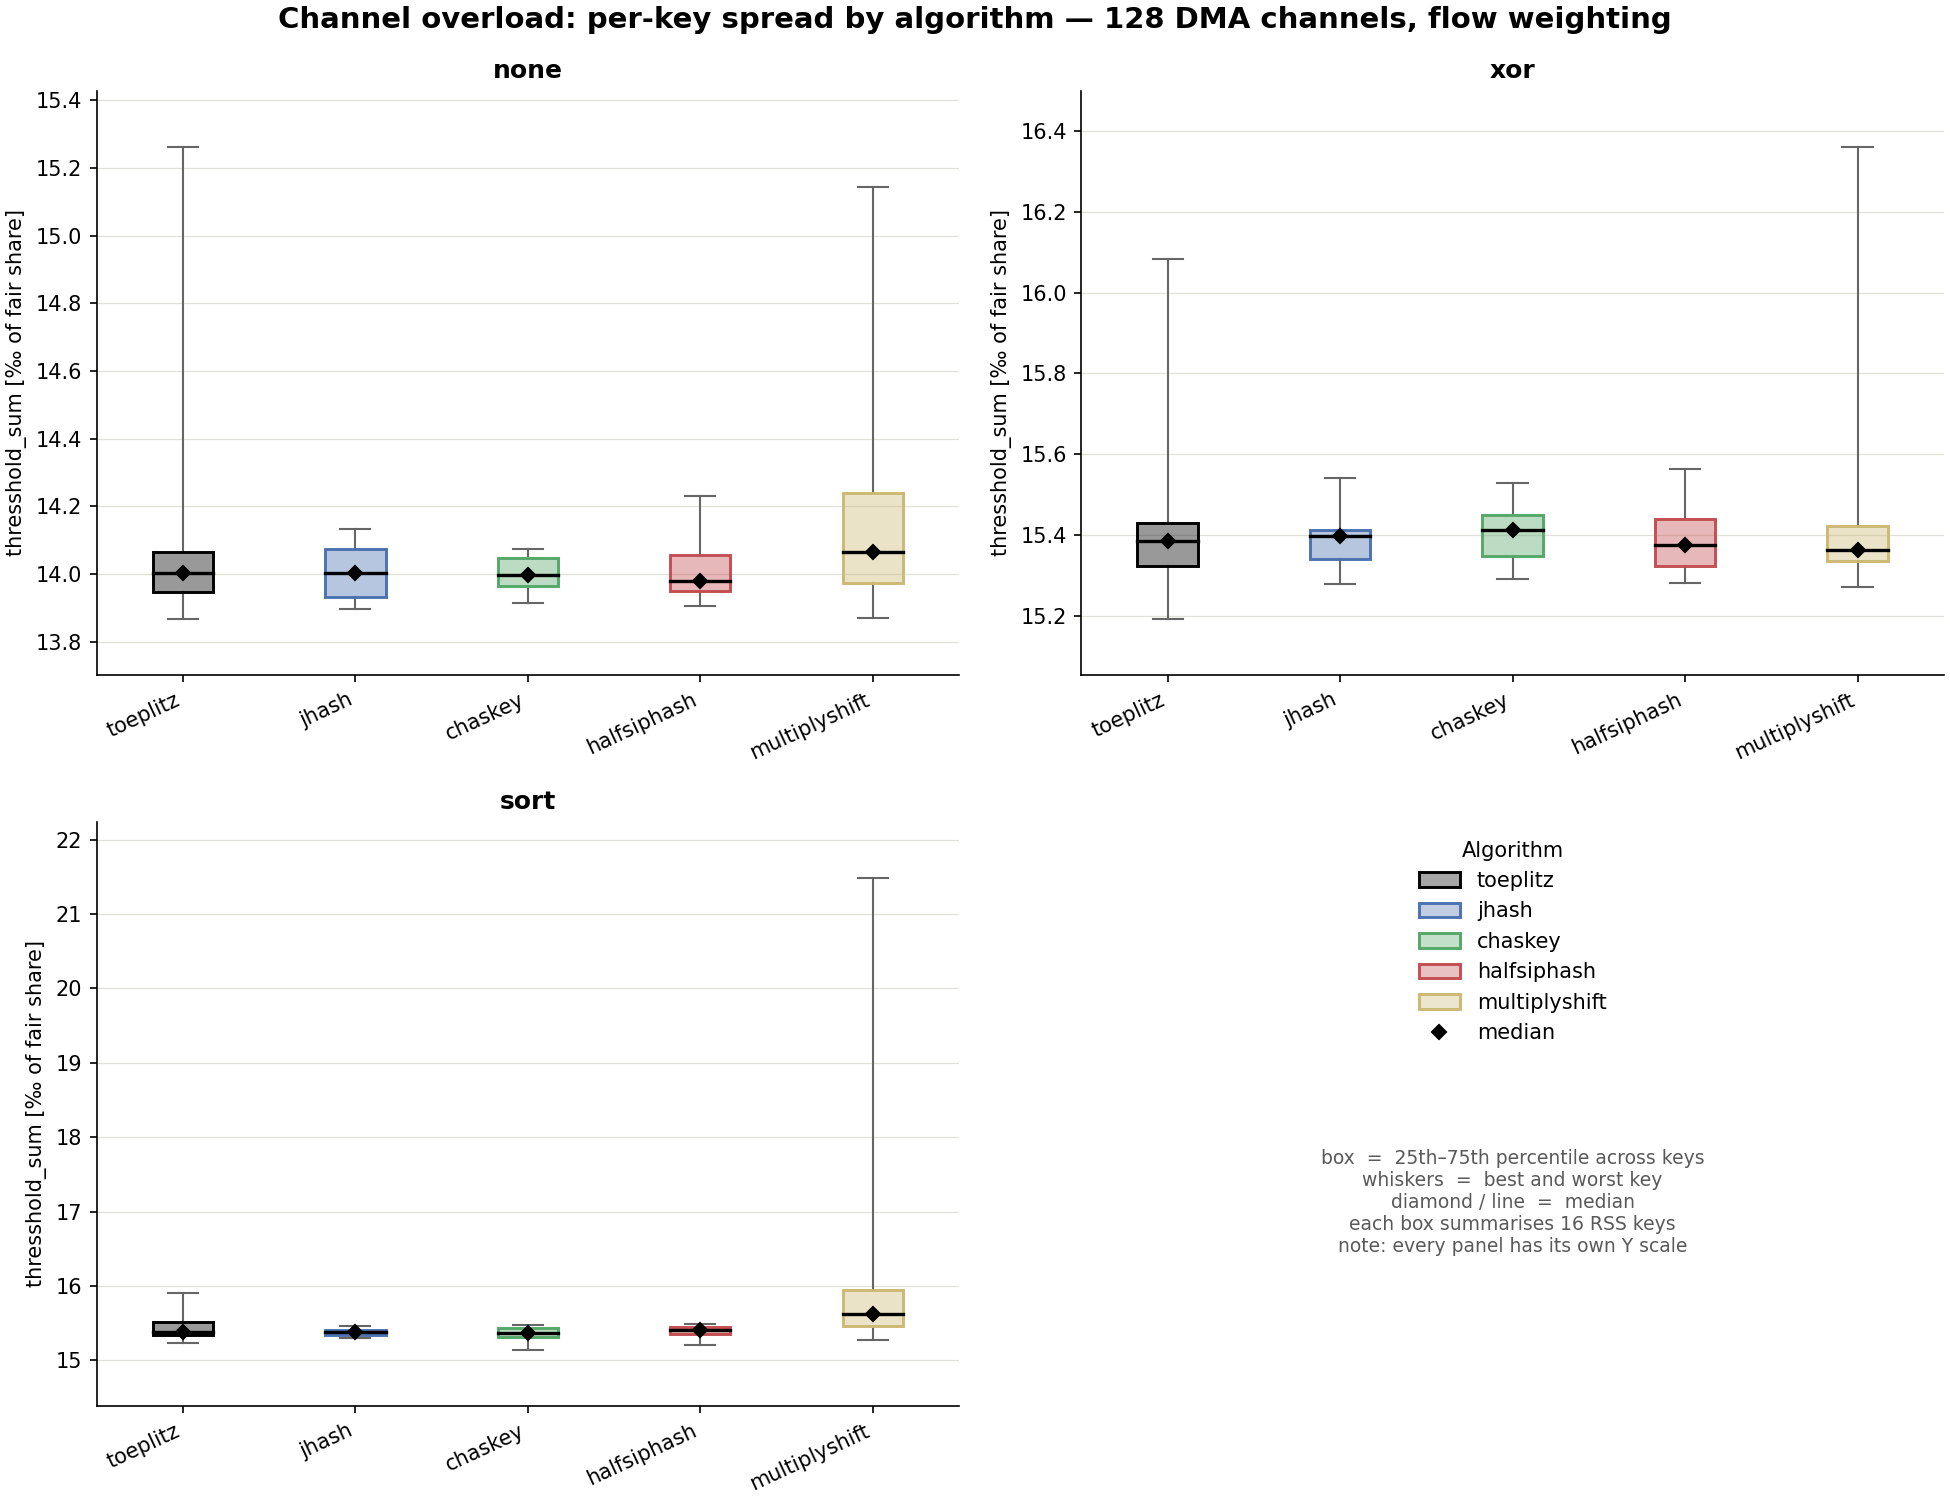
\includegraphics[width=\textwidth]{ostatne_vzorky/odid2_full_tuple/keys_128.png}
    \caption{128 kanálov}
  \end{subfigure}

  \caption{Rozptyl preťaženia medzi 16 kľúčmi pri váhe \texttt{flow}: \texttt{odid2}, plný tuple.}
  \label{fig:b-odid2-full-tuple-keys}
\end{figure}

\begin{figure}[ht]
  \centering
  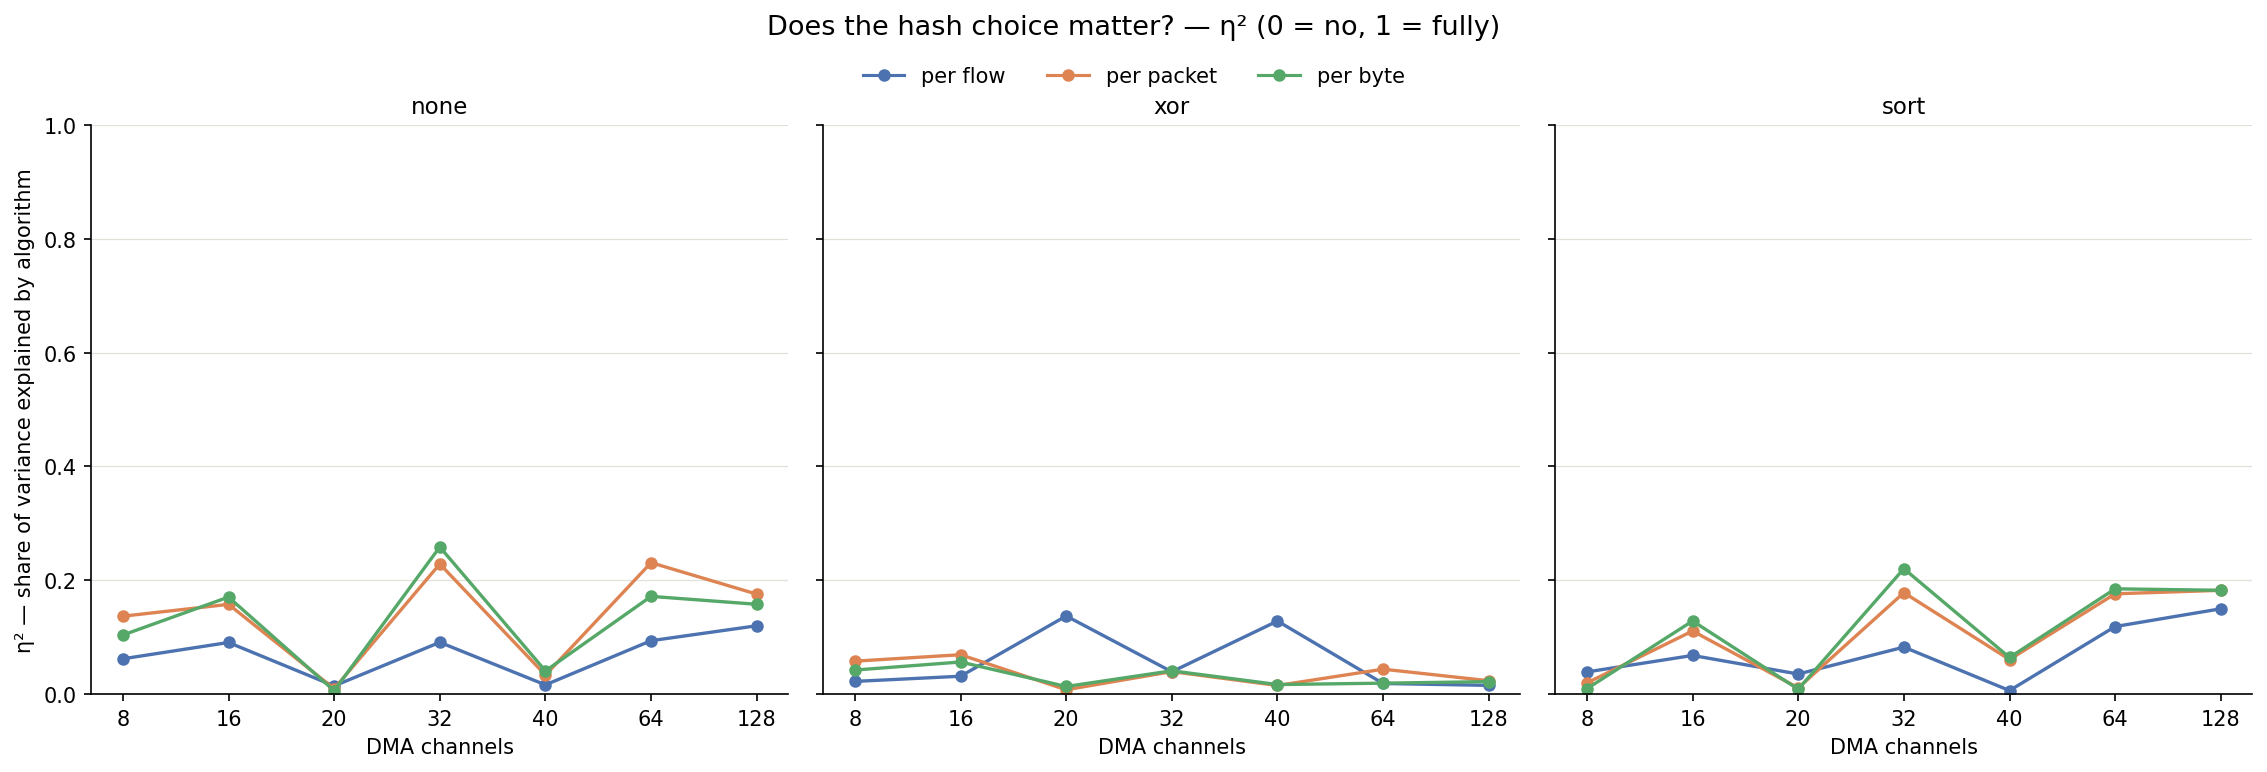
\includegraphics[width=0.9\textwidth]{ostatne_vzorky/odid2_full_tuple/spread.png}
  \caption{Podiel rozptylu vysvetlený voľbou funkcie ($\eta^2$): \texttt{odid2}, plný tuple.}
  \label{fig:b-odid2-full-tuple-spread}
\end{figure}

\clearpage
\begin{figure}[p]
  \centering
  \begin{subfigure}{0.60\textwidth}
    \centering
    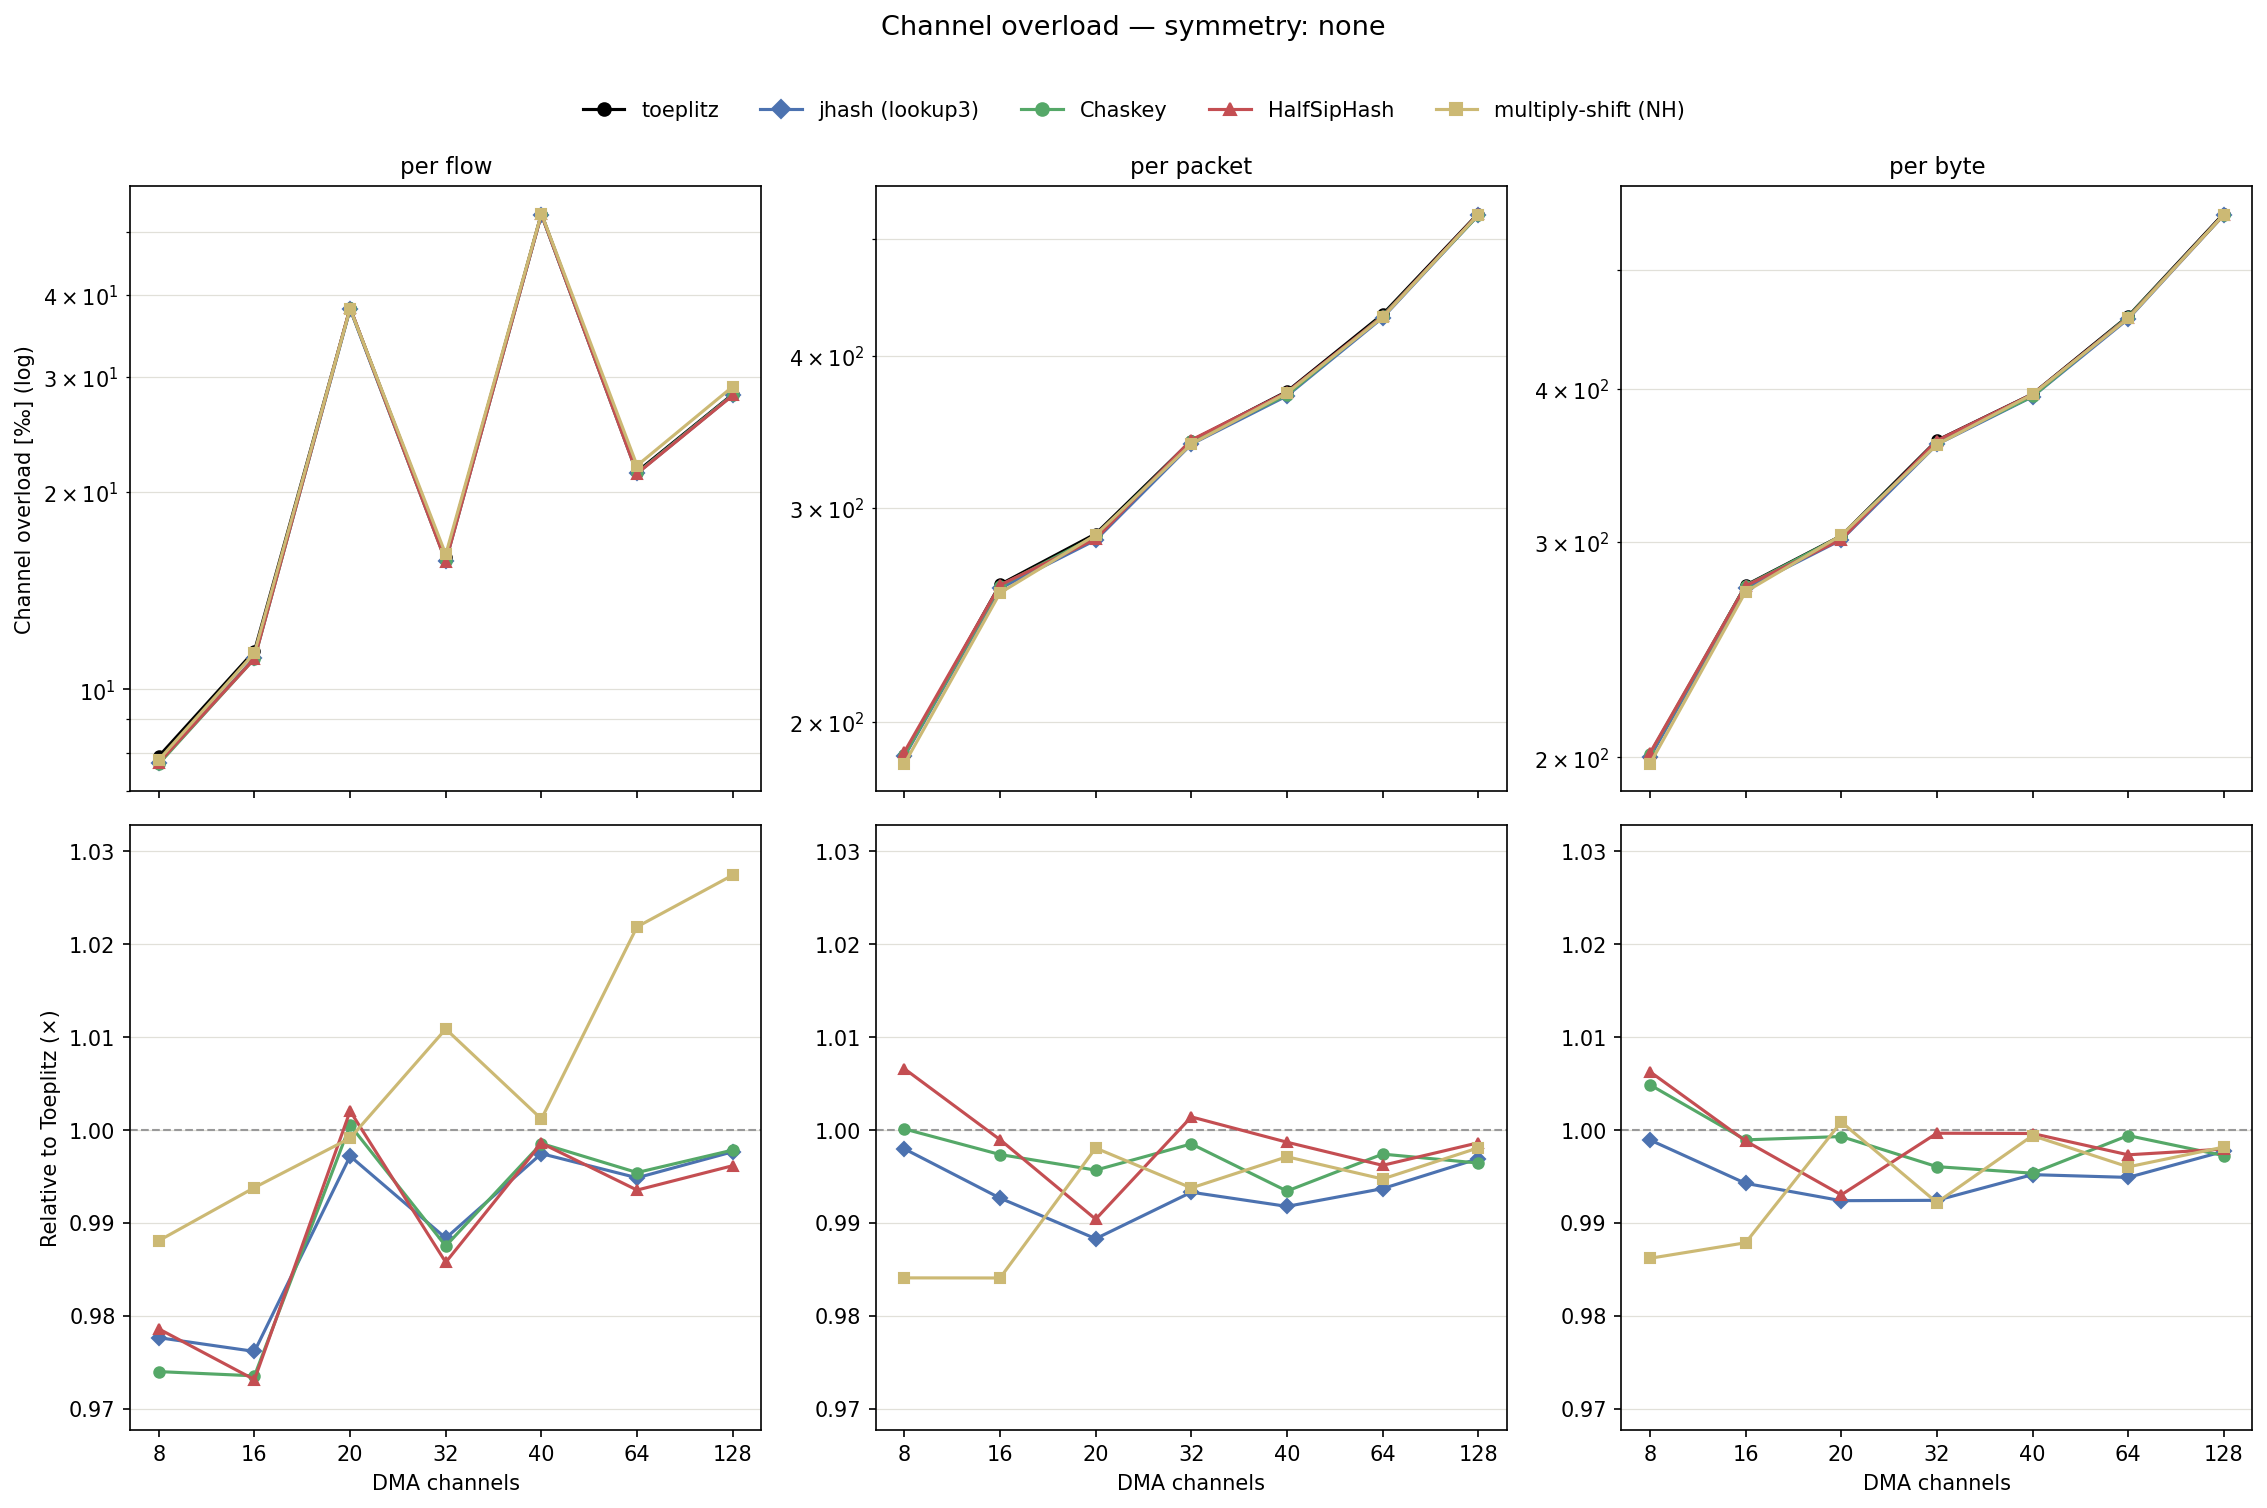
\includegraphics[width=\textwidth]{ostatne_vzorky/odid4_full_tuple/overload_none.png}
    \caption{bez symetrie}
  \end{subfigure}

  \begin{subfigure}{0.60\textwidth}
    \centering
    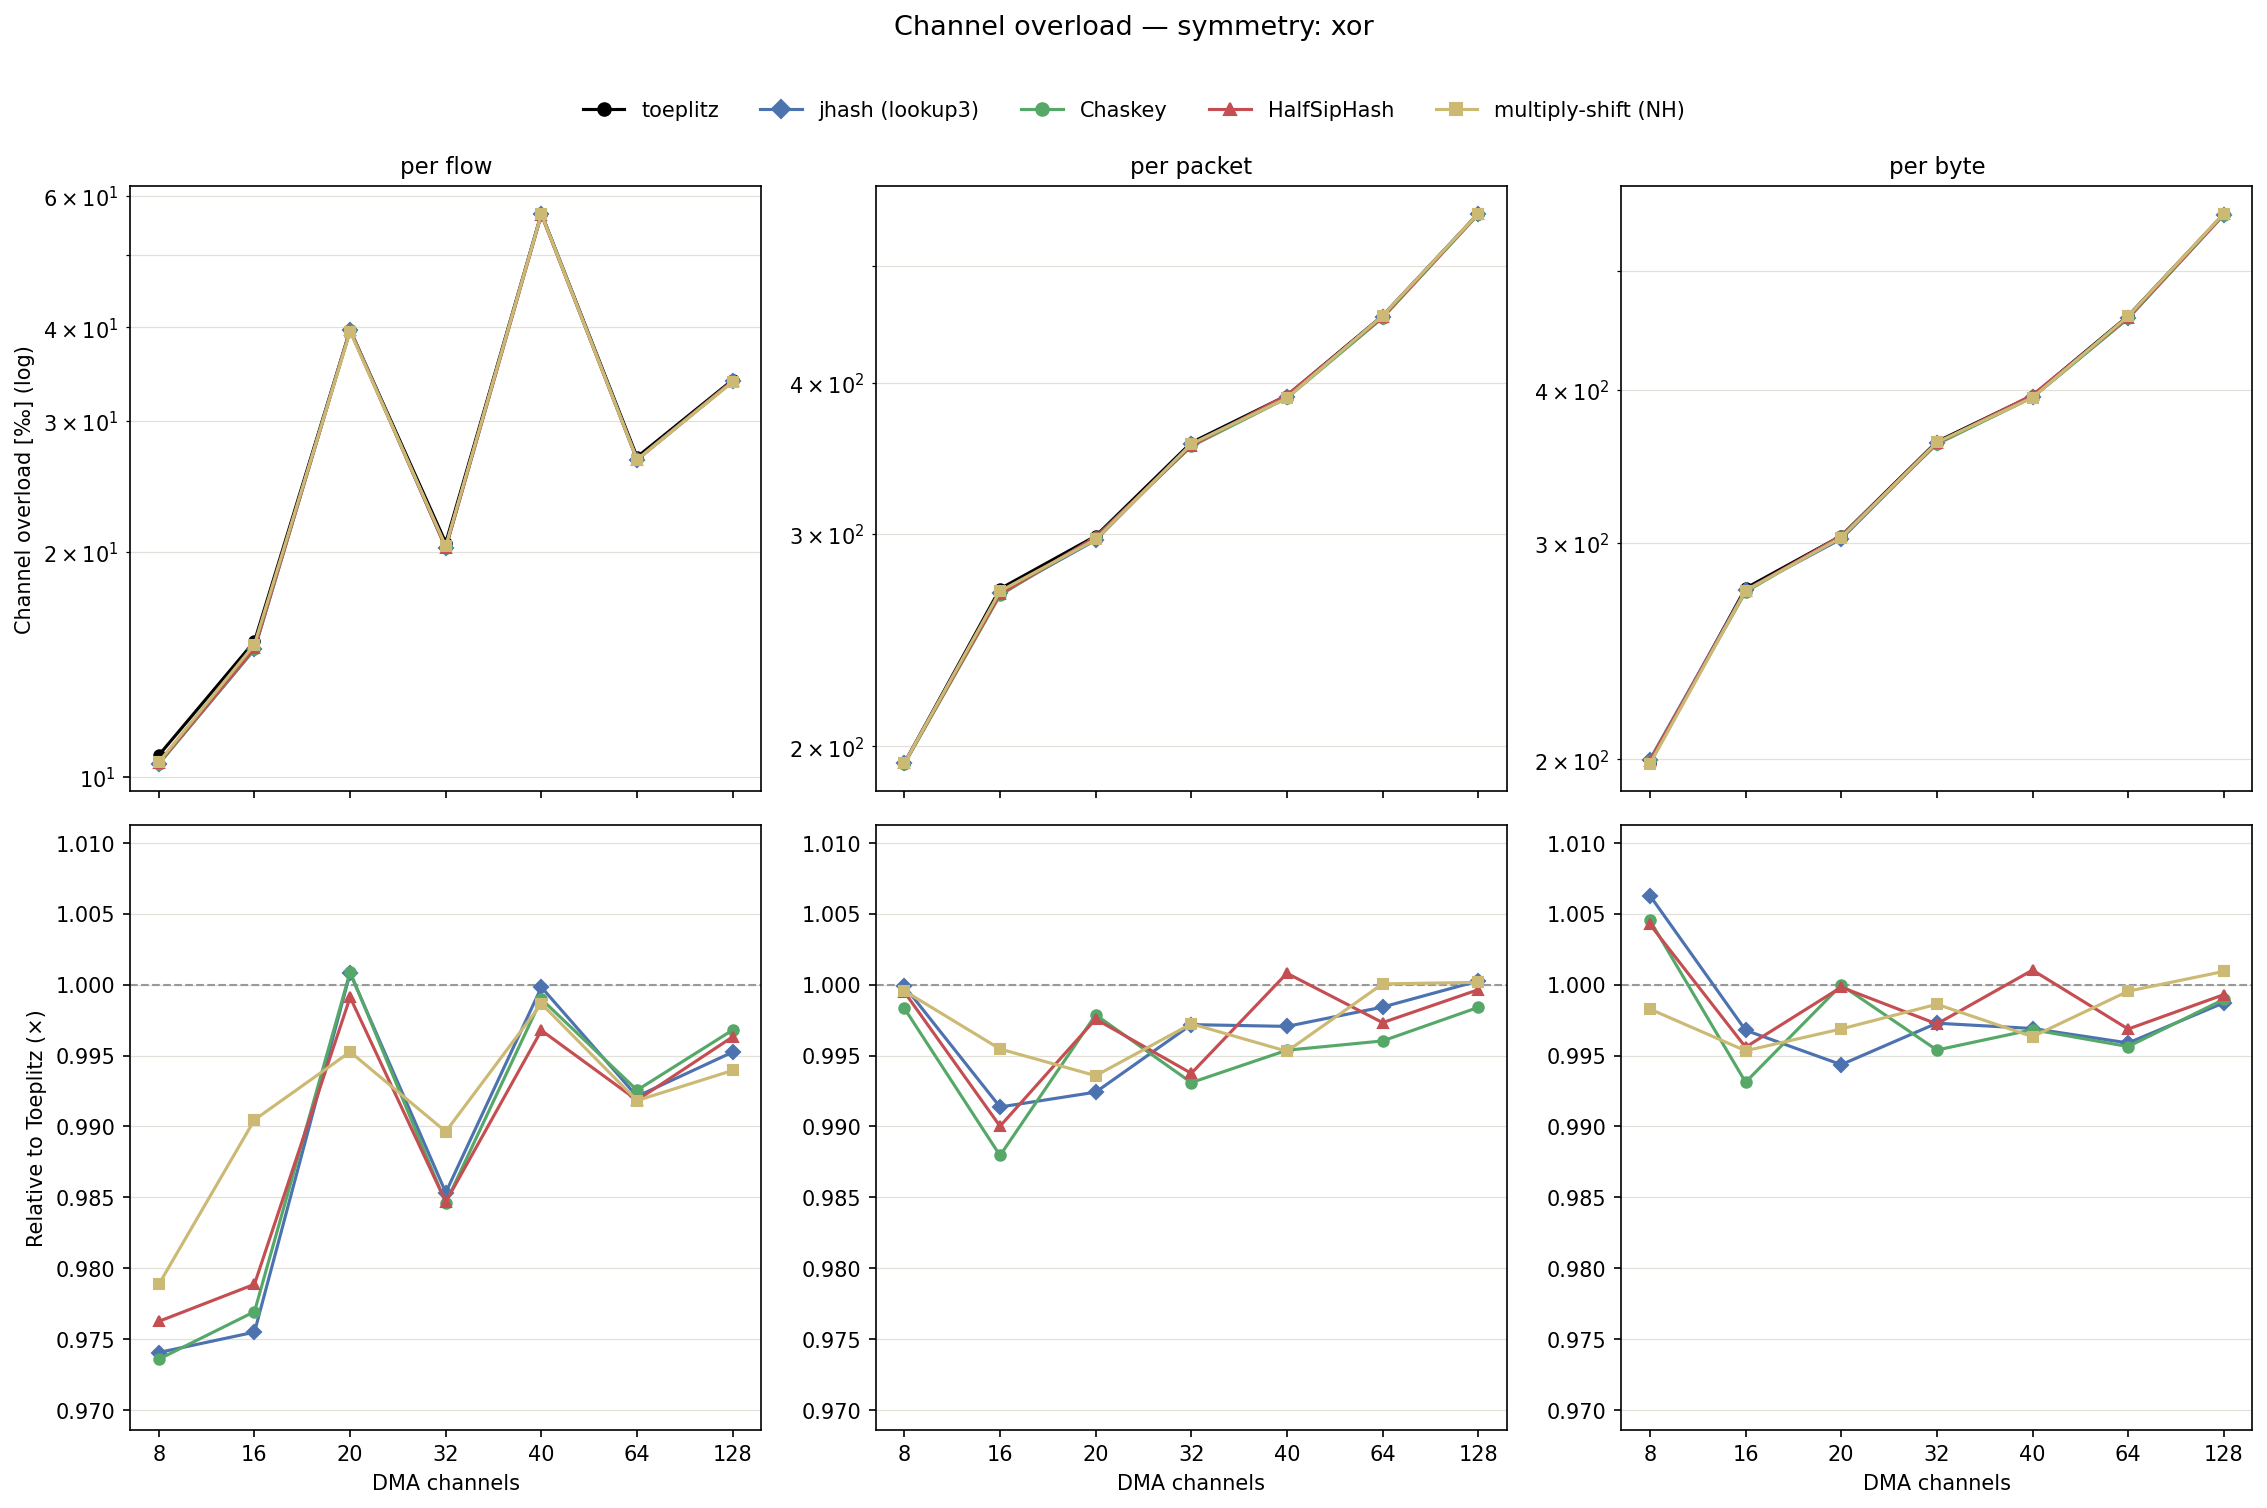
\includegraphics[width=\textwidth]{ostatne_vzorky/odid4_full_tuple/overload_xorfold.png}
    \caption{symetria XOR}
  \end{subfigure}

  \begin{subfigure}{0.60\textwidth}
    \centering
    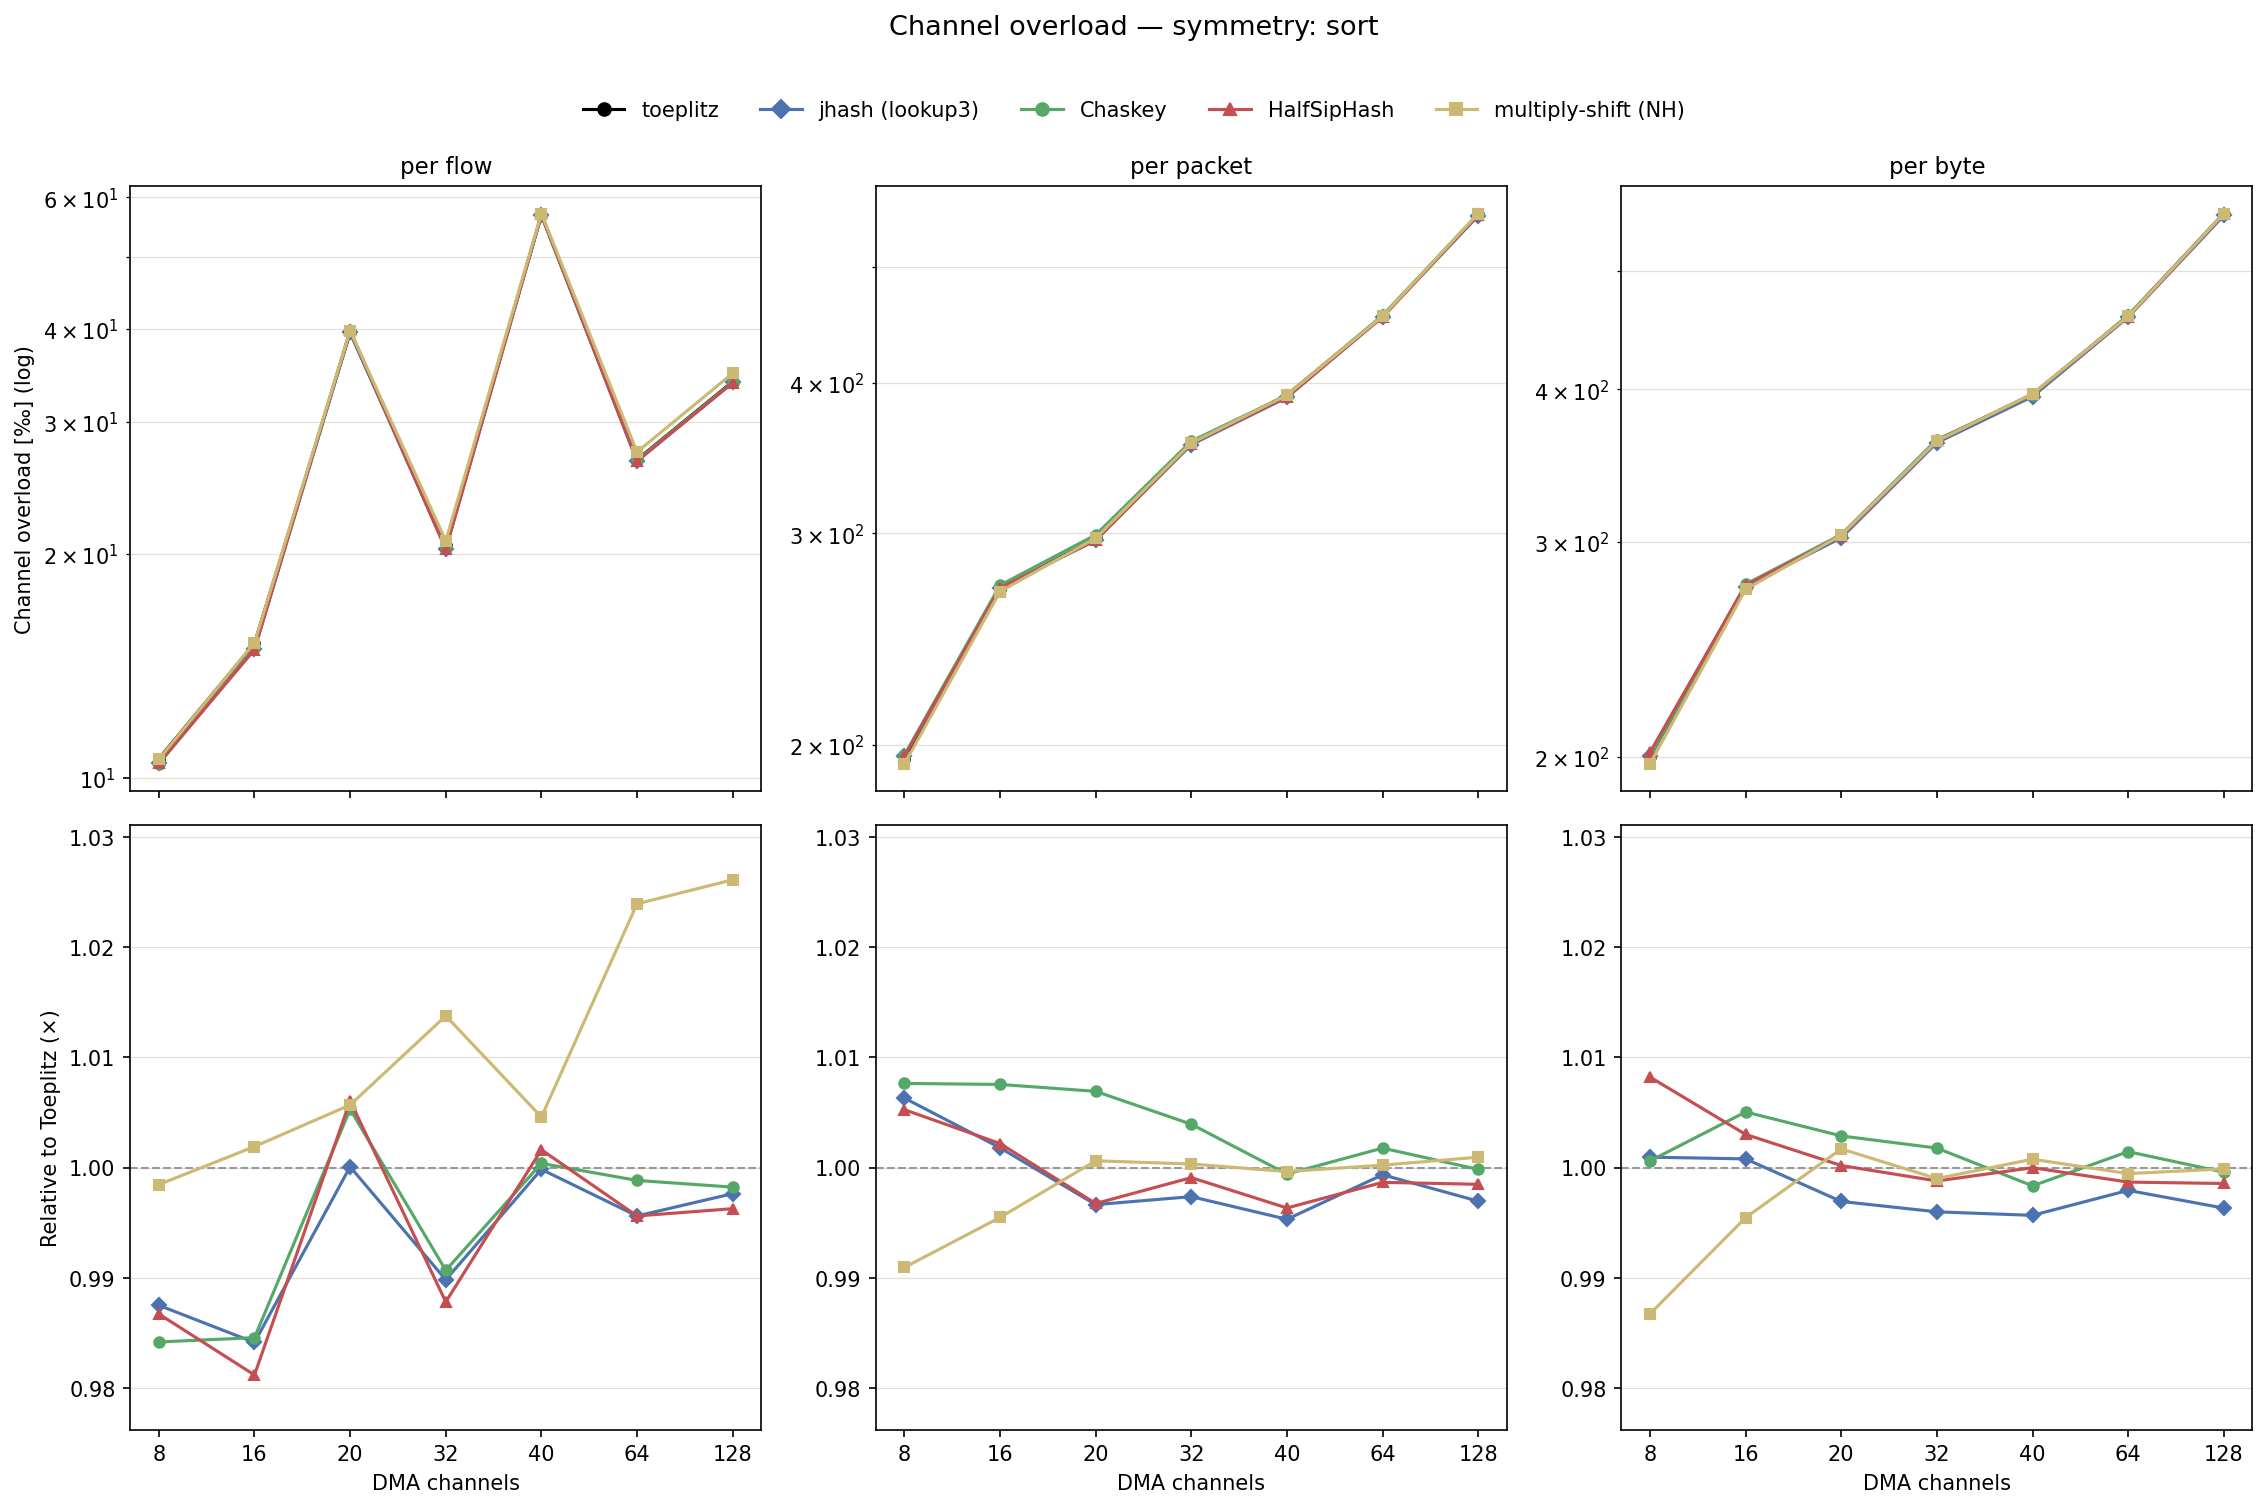
\includegraphics[width=\textwidth]{ostatne_vzorky/odid4_full_tuple/overload_sortfold.png}
    \caption{symetria sort}
  \end{subfigure}

  \caption{Preťaženie funkcií a pomer k~Toeplitzu: \texttt{odid4}, plný tuple.}
  \label{fig:b-odid4-full-tuple-overload}
\end{figure}

\begin{figure}[p]
  \centering
  \begin{subfigure}{0.54\textwidth}
    \centering
    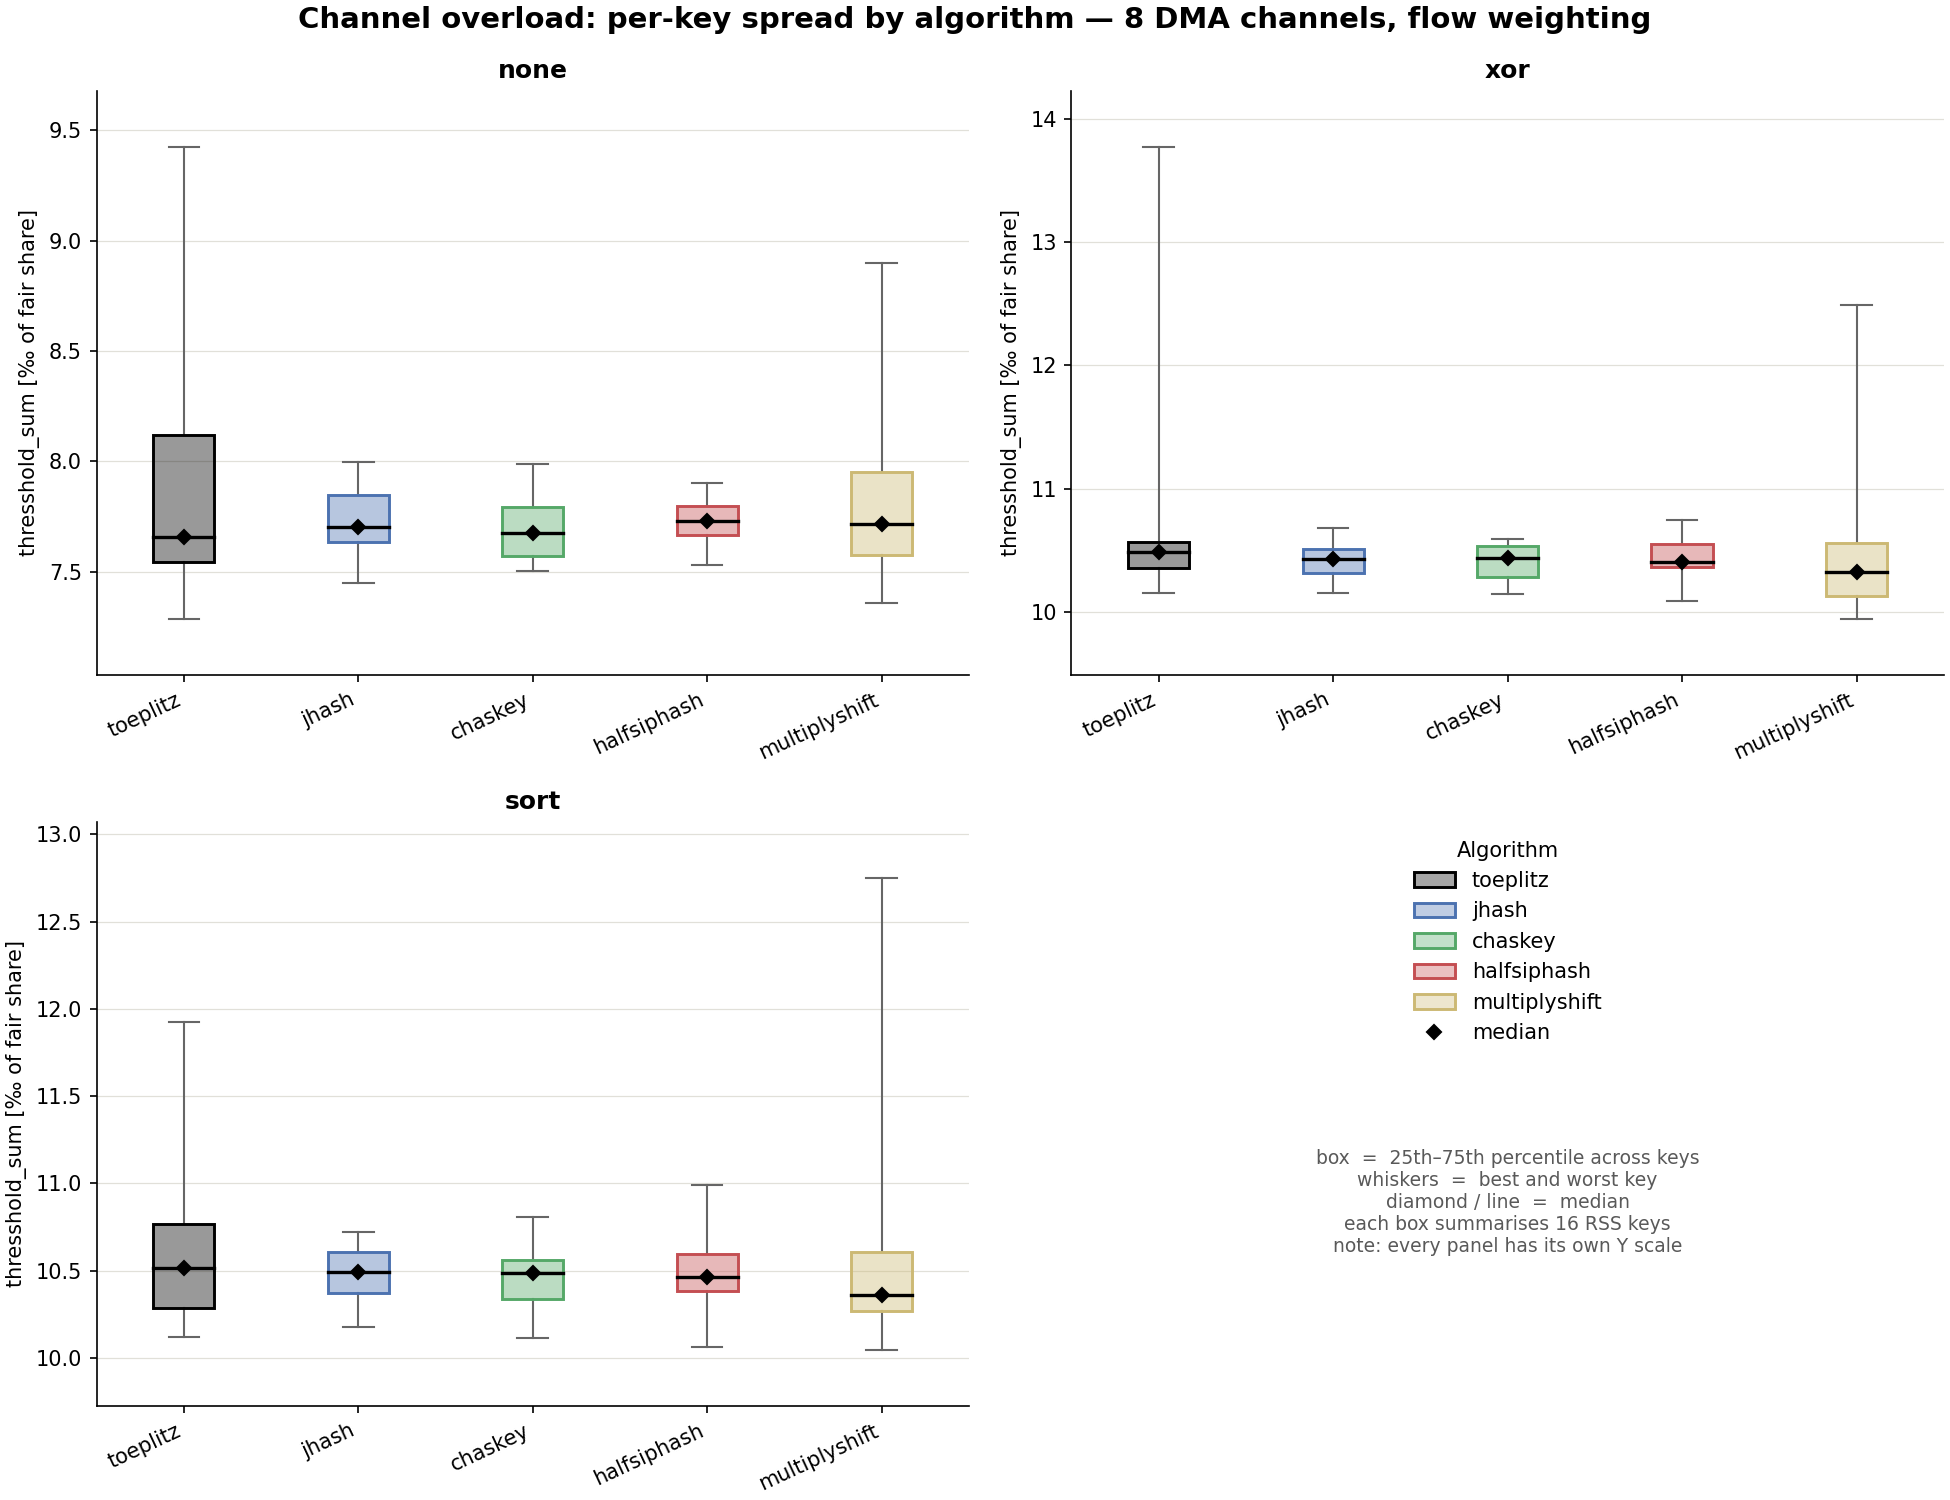
\includegraphics[width=\textwidth]{ostatne_vzorky/odid4_full_tuple/keys_8.png}
    \caption{8 kanálov}
  \end{subfigure}

  \begin{subfigure}{0.54\textwidth}
    \centering
    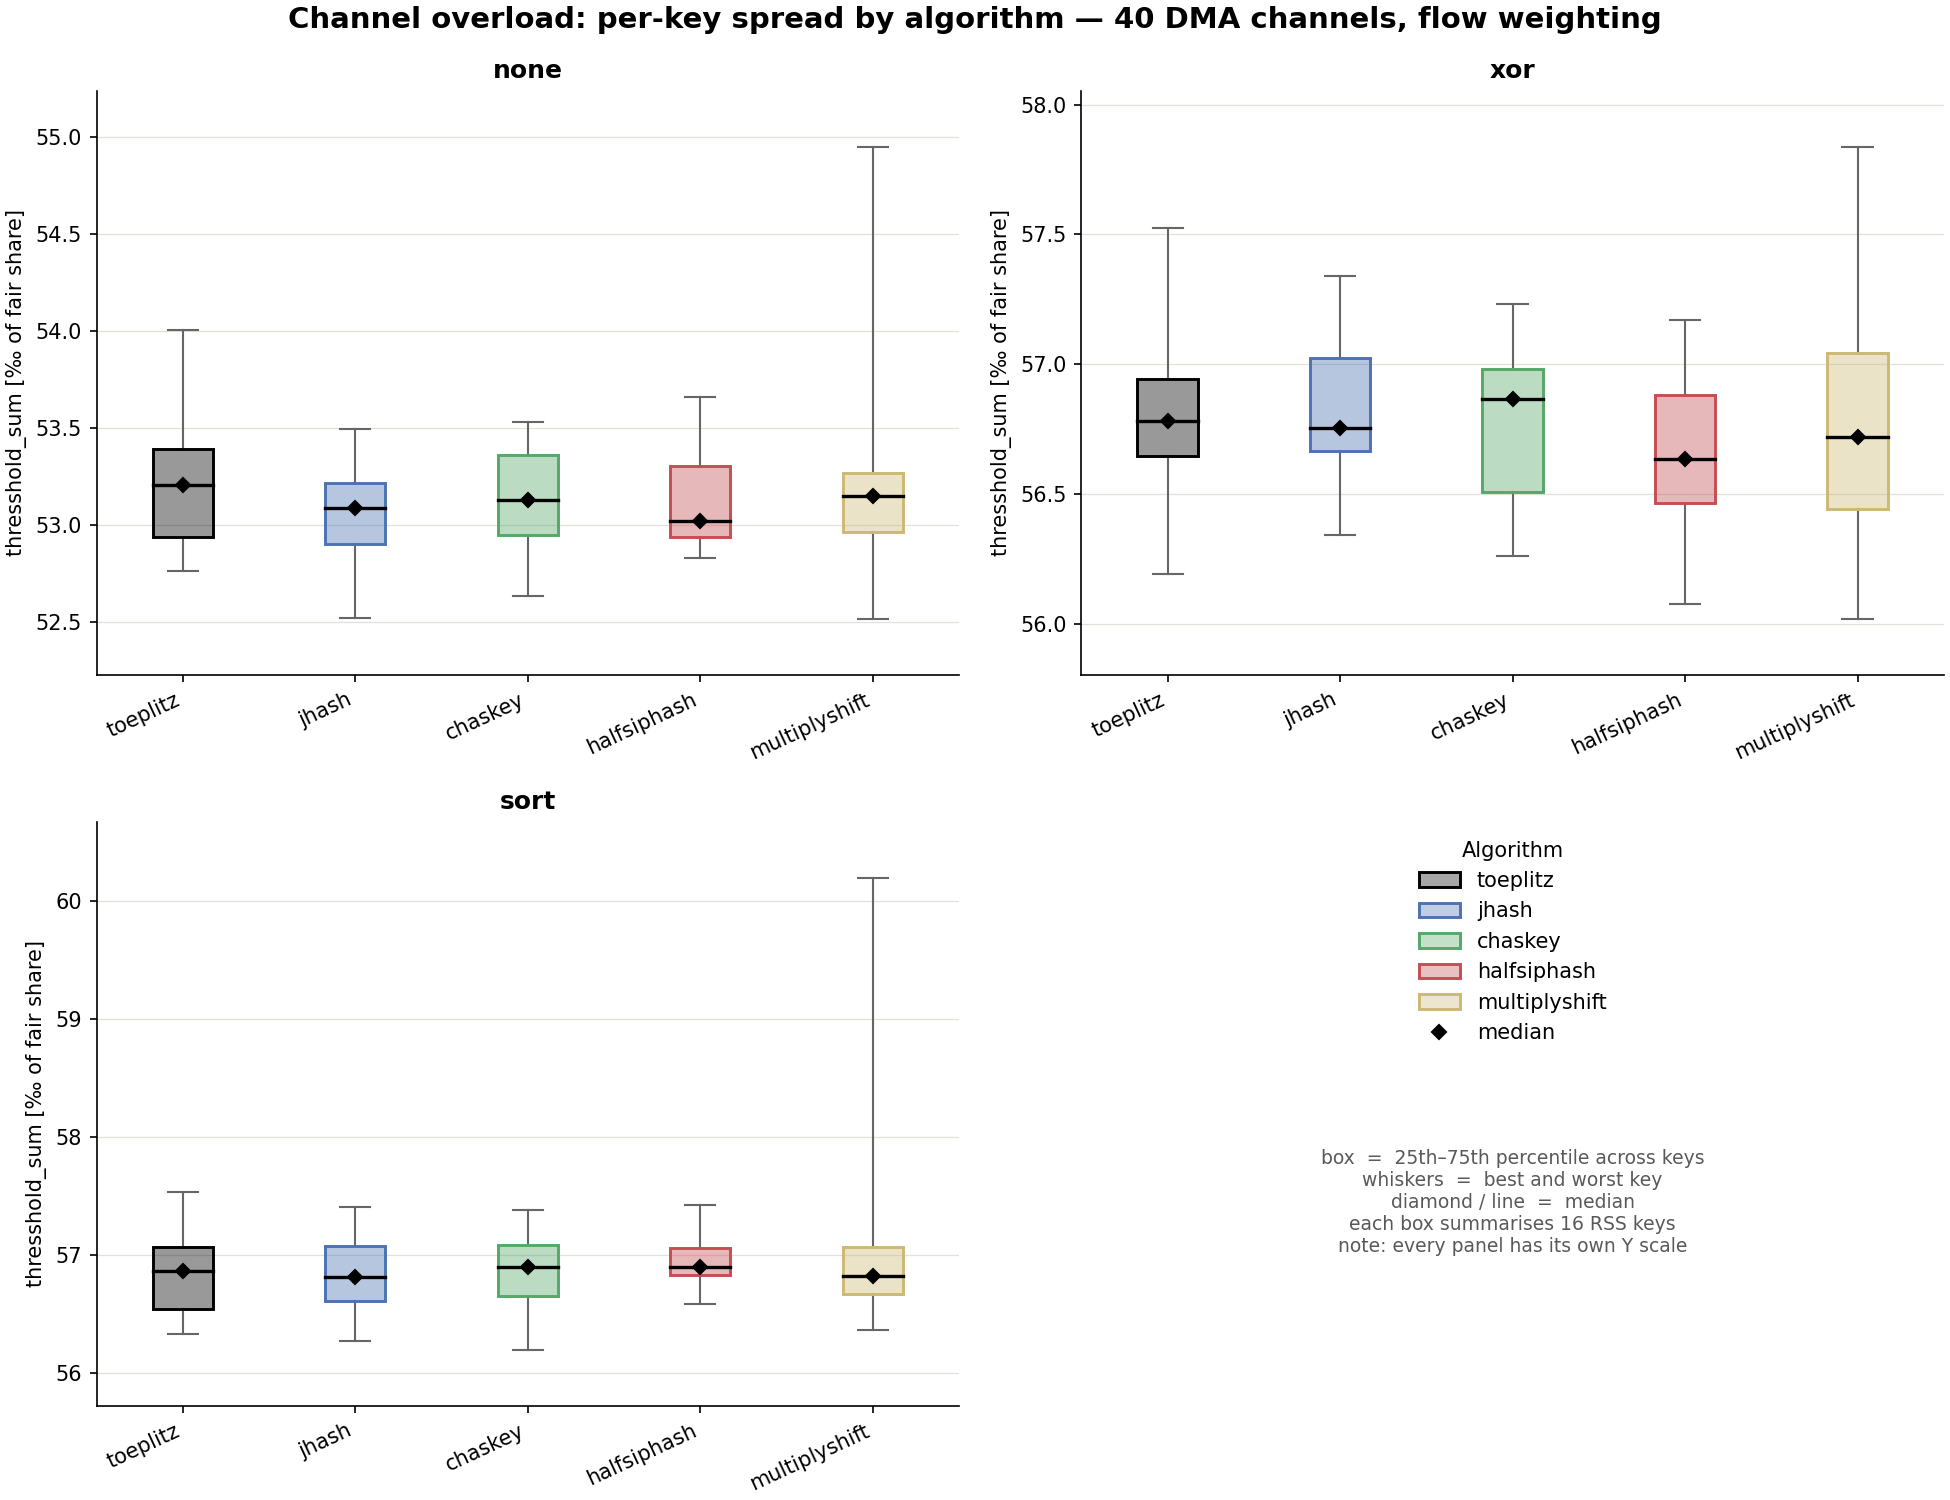
\includegraphics[width=\textwidth]{ostatne_vzorky/odid4_full_tuple/keys_40.png}
    \caption{40 kanálov}
  \end{subfigure}

  \begin{subfigure}{0.54\textwidth}
    \centering
    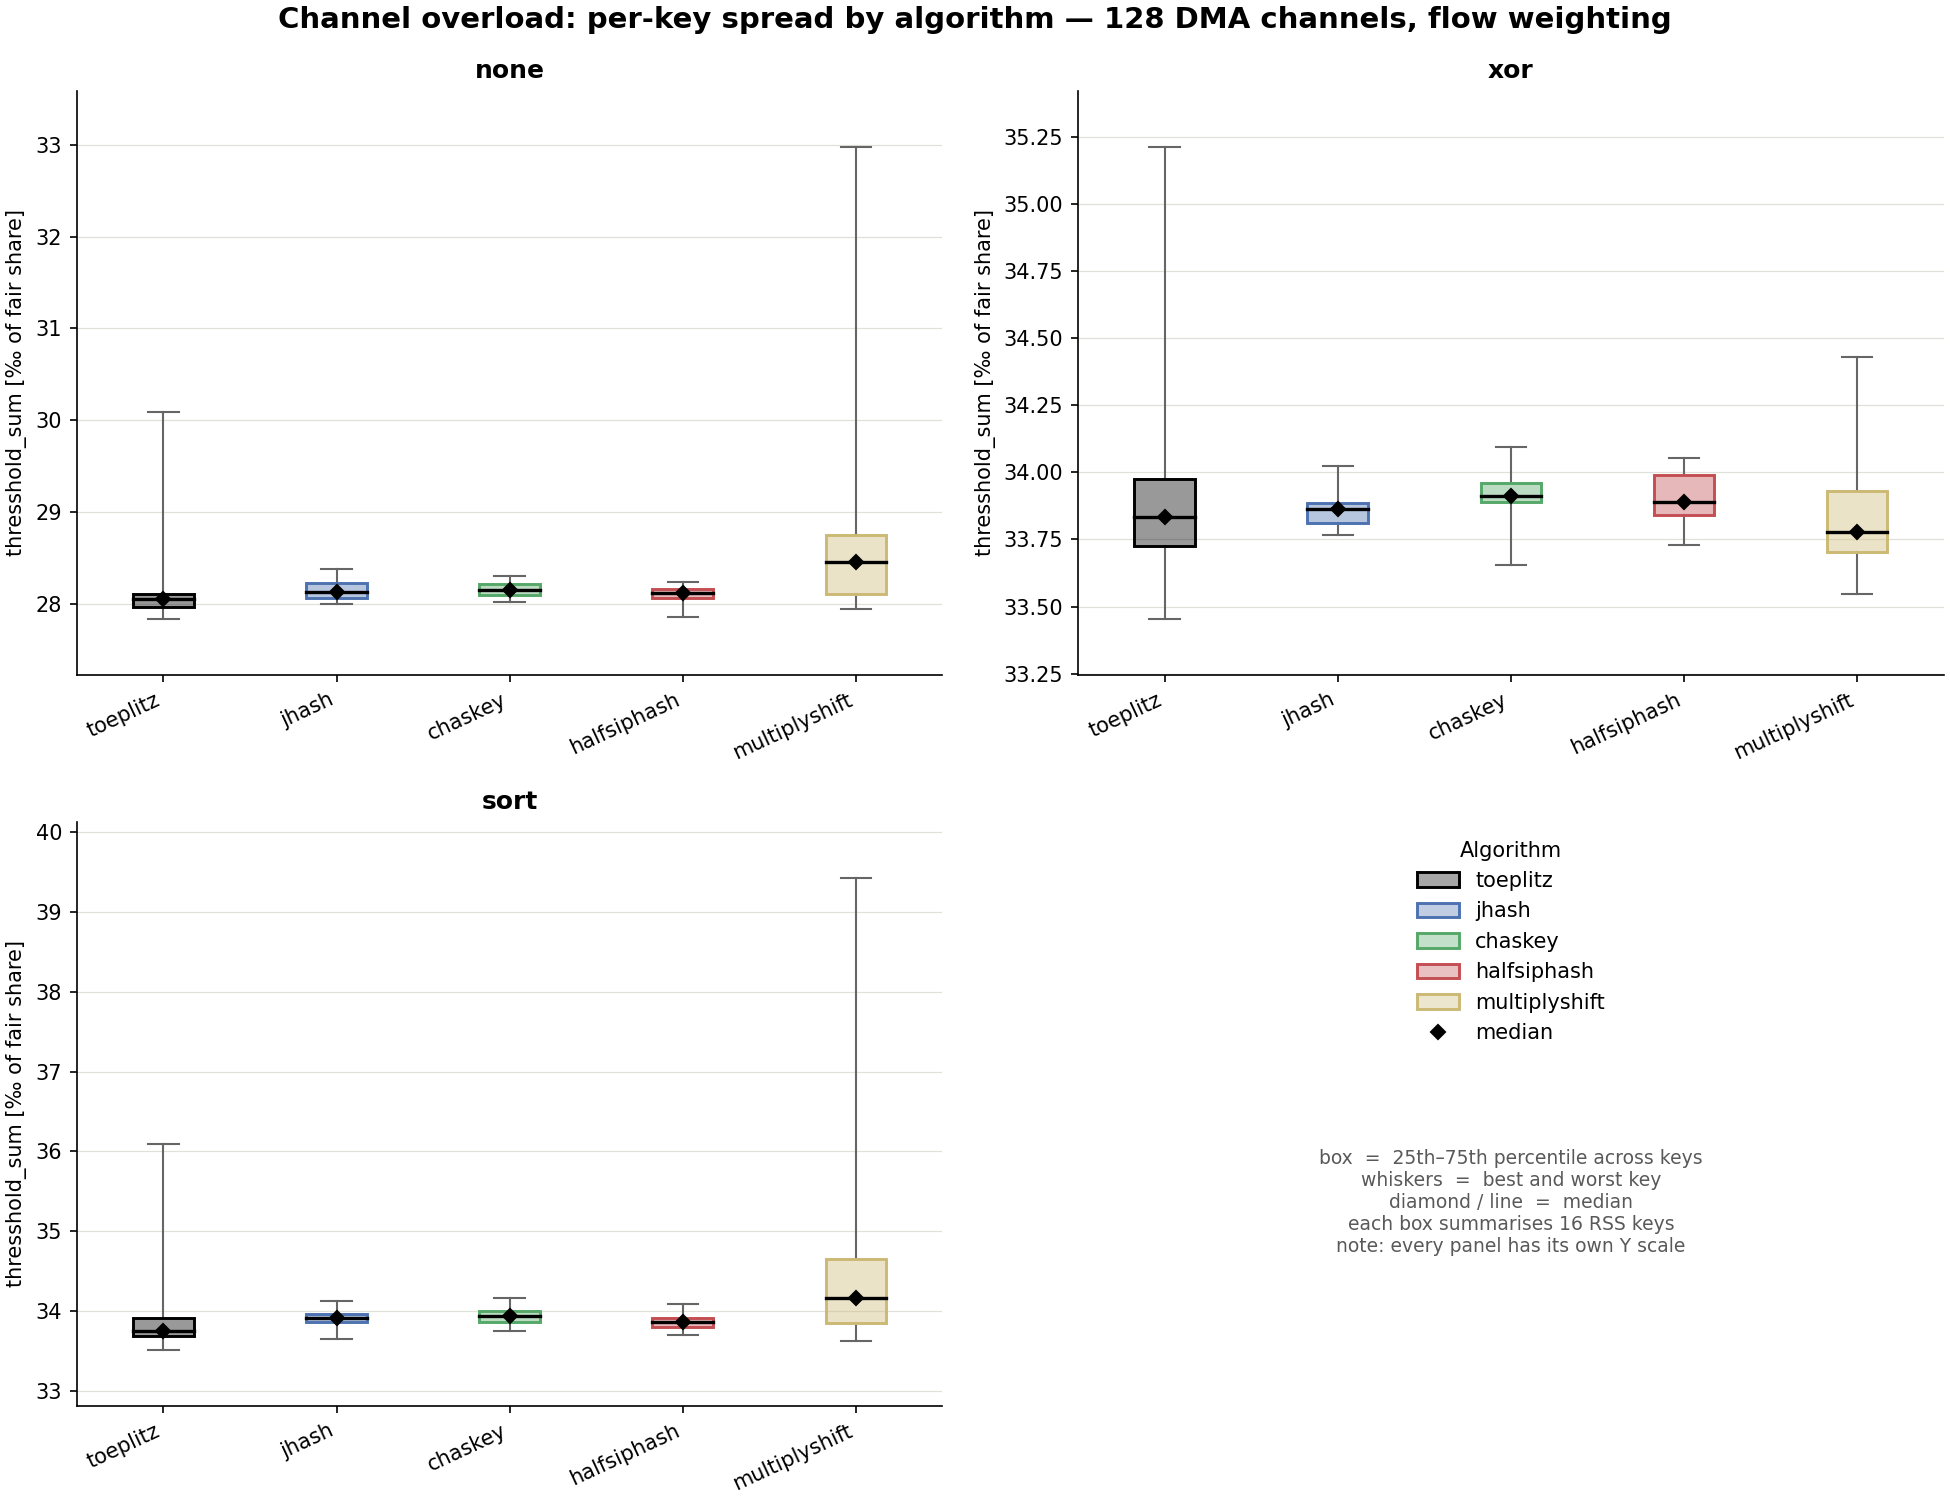
\includegraphics[width=\textwidth]{ostatne_vzorky/odid4_full_tuple/keys_128.png}
    \caption{128 kanálov}
  \end{subfigure}

  \caption{Rozptyl preťaženia medzi 16 kľúčmi pri váhe \texttt{flow}: \texttt{odid4}, plný tuple.}
  \label{fig:b-odid4-full-tuple-keys}
\end{figure}

\begin{figure}[ht]
  \centering
  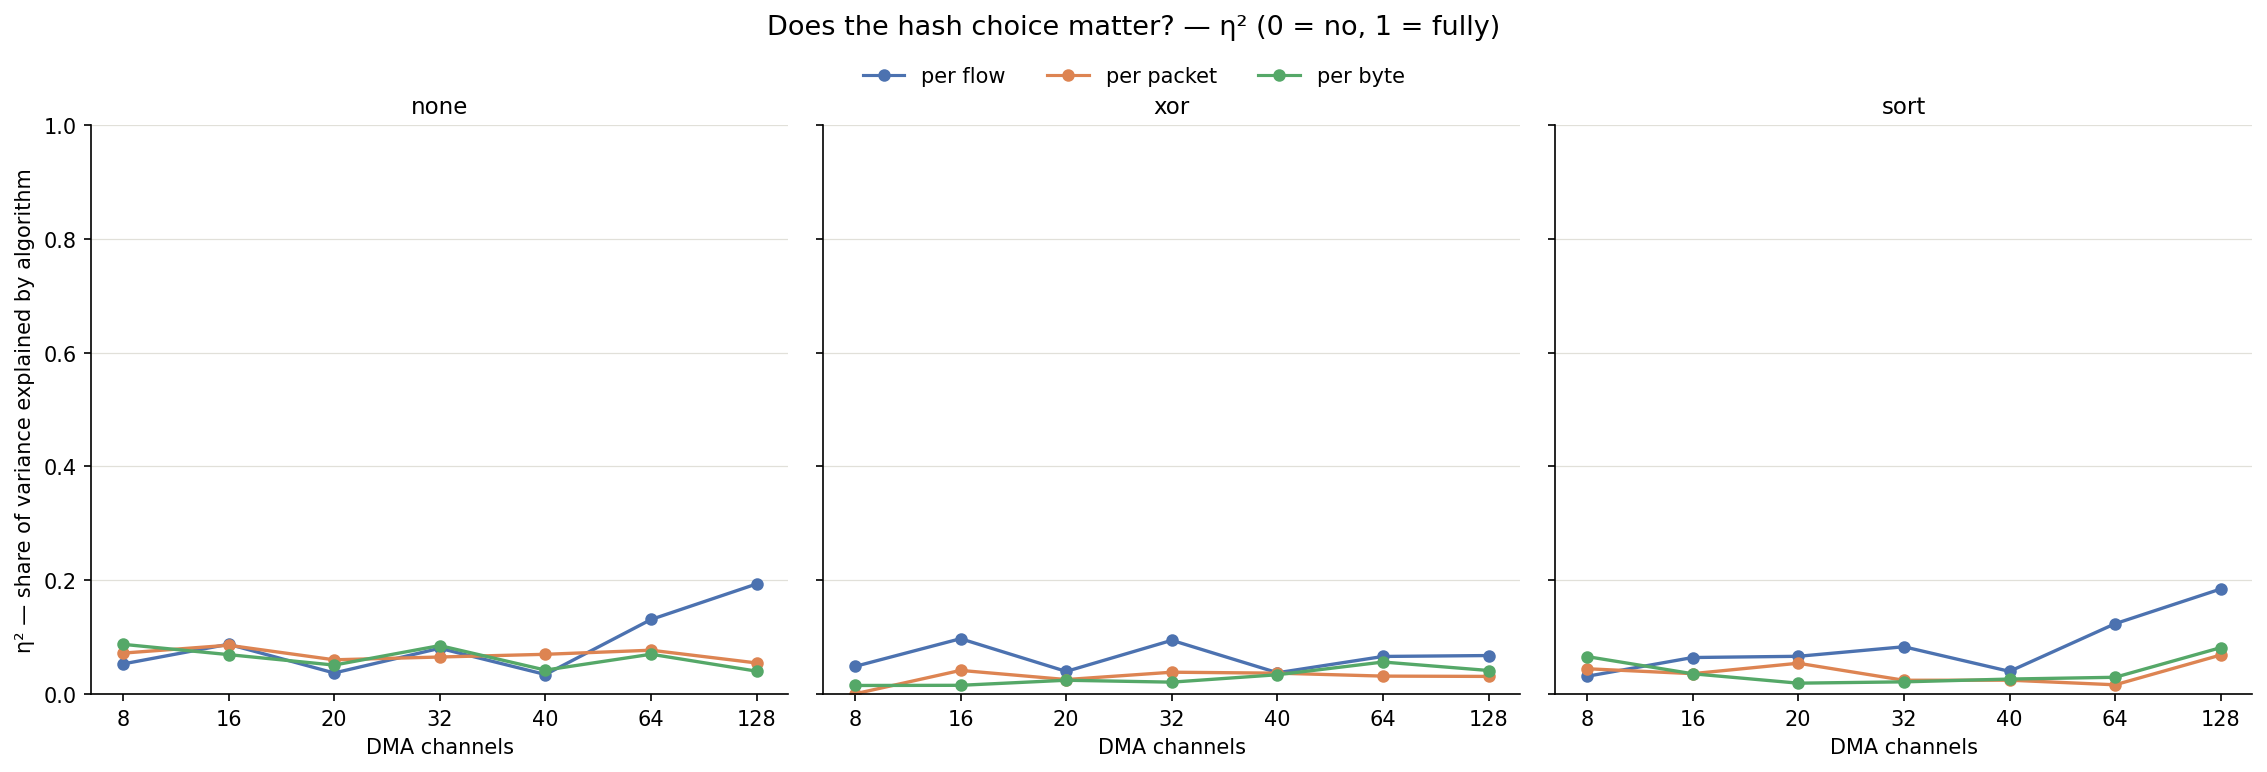
\includegraphics[width=0.9\textwidth]{ostatne_vzorky/odid4_full_tuple/spread.png}
  \caption{Podiel rozptylu vysvetlený voľbou funkcie ($\eta^2$): \texttt{odid4}, plný tuple.}
  \label{fig:b-odid4-full-tuple-spread}
\end{figure}

\clearpage
\begin{figure}[p]
  \centering
  \begin{subfigure}{0.60\textwidth}
    \centering
    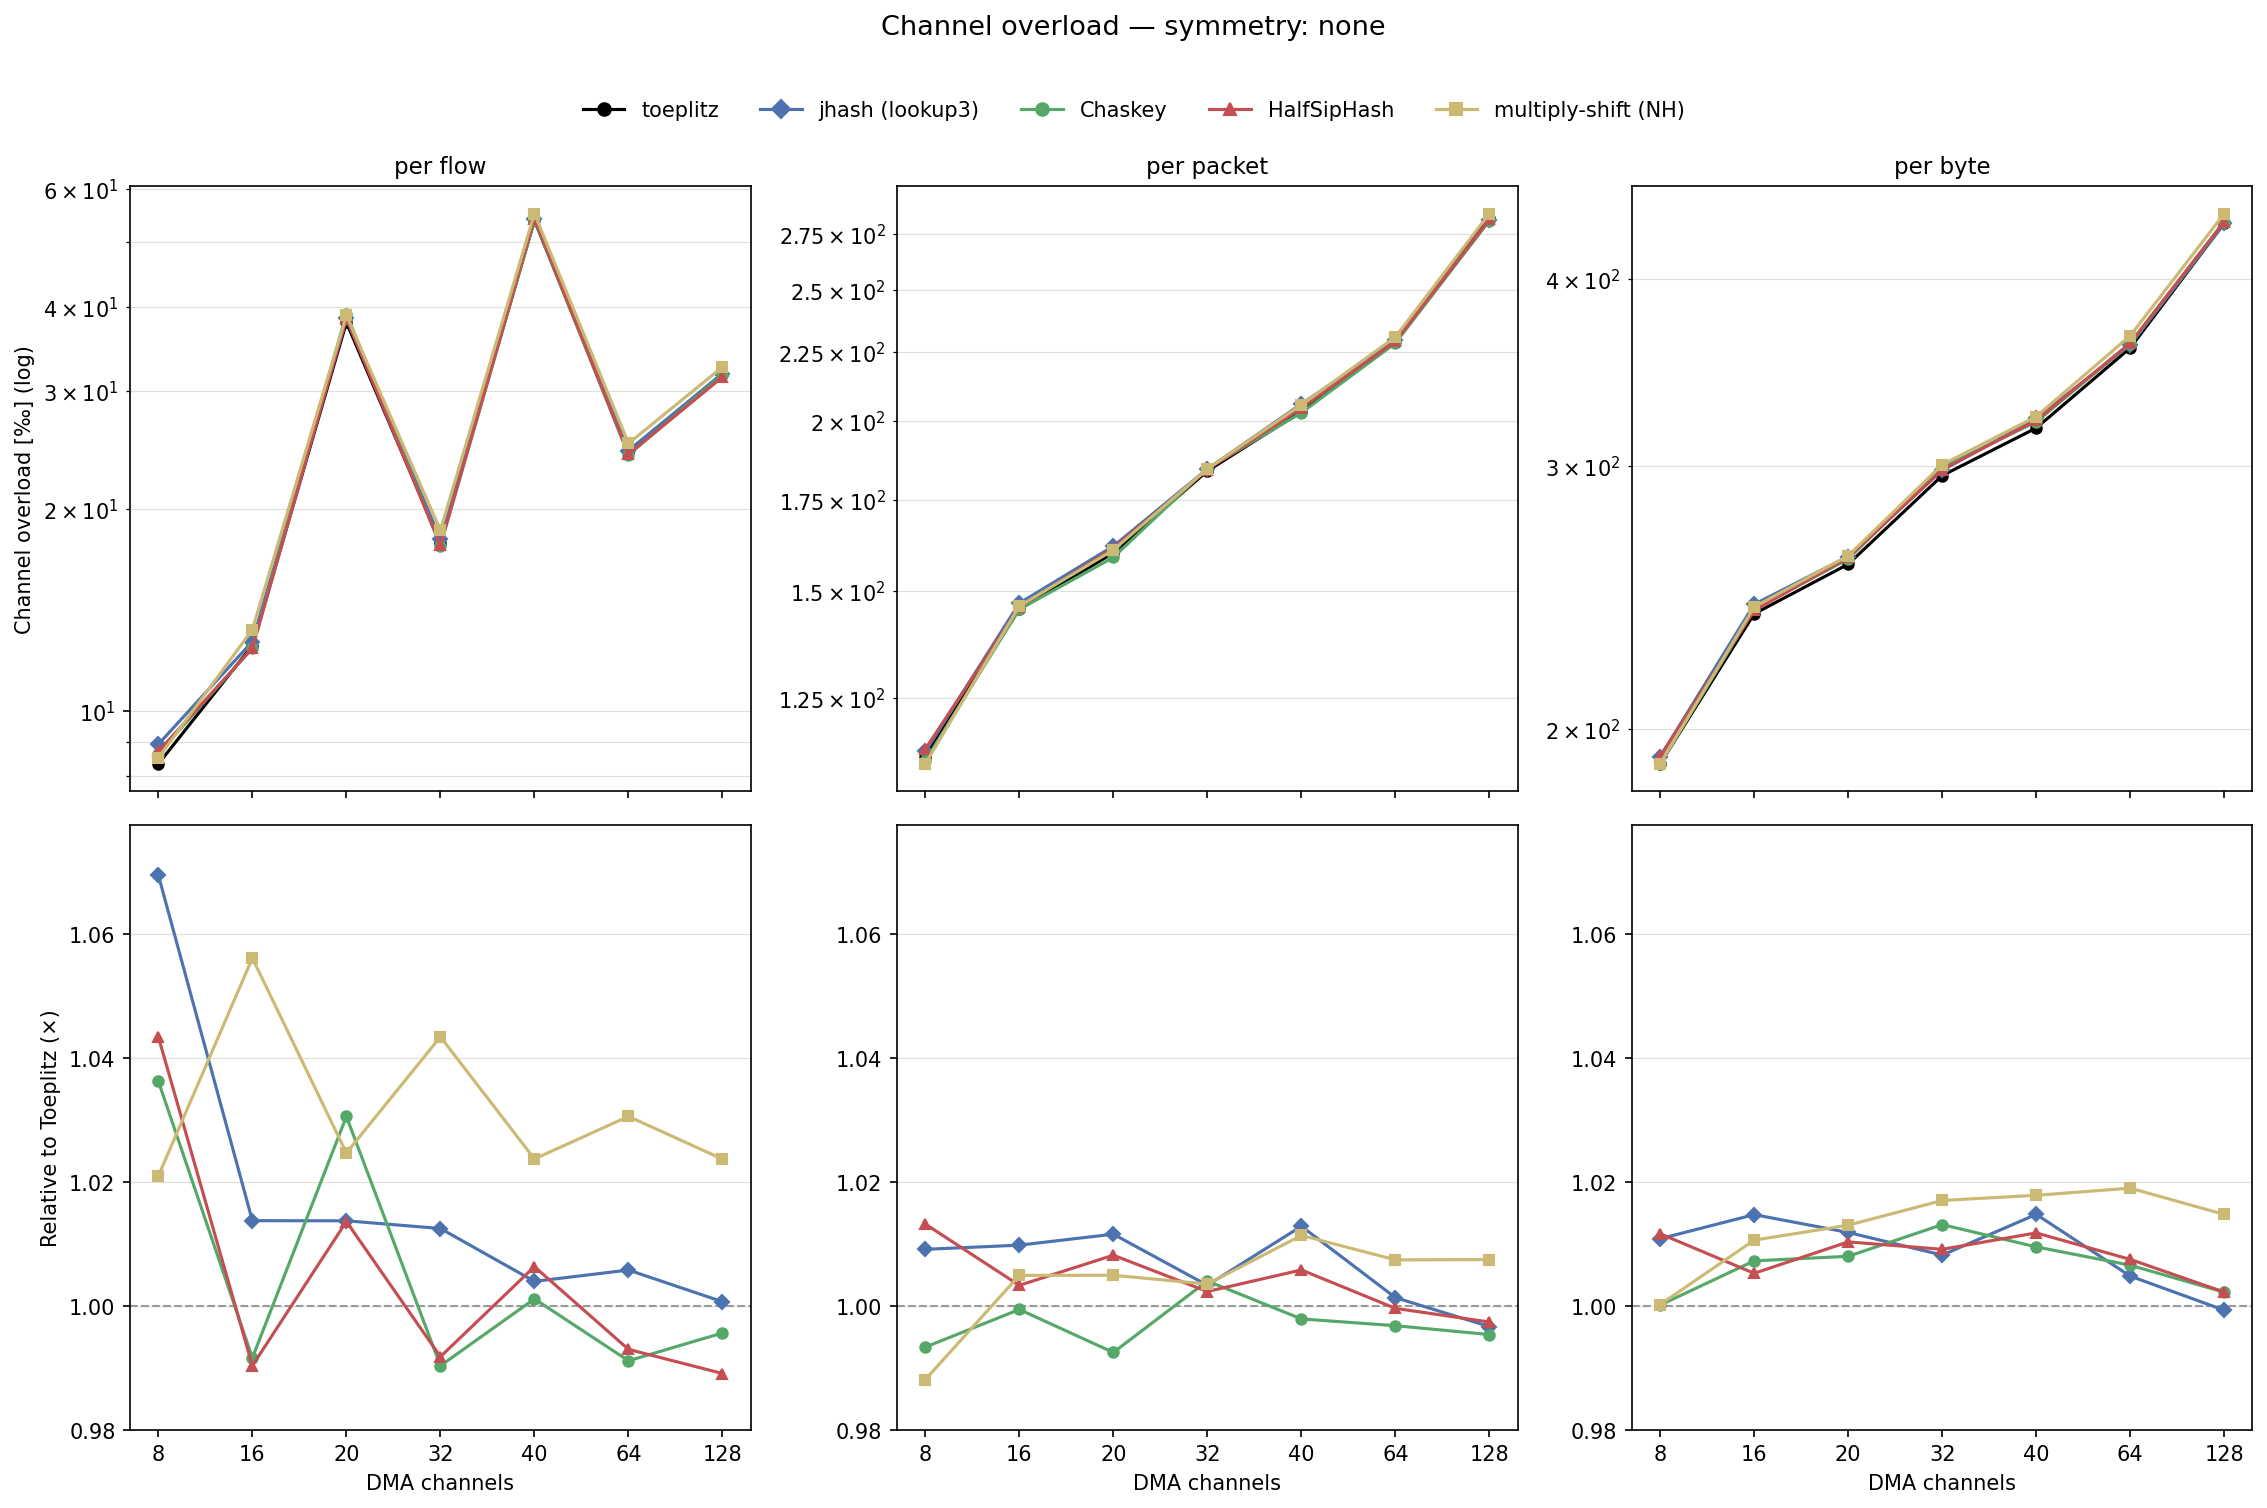
\includegraphics[width=\textwidth]{ostatne_vzorky/odid6_full_tuple/overload_none.png}
    \caption{bez symetrie}
  \end{subfigure}

  \begin{subfigure}{0.60\textwidth}
    \centering
    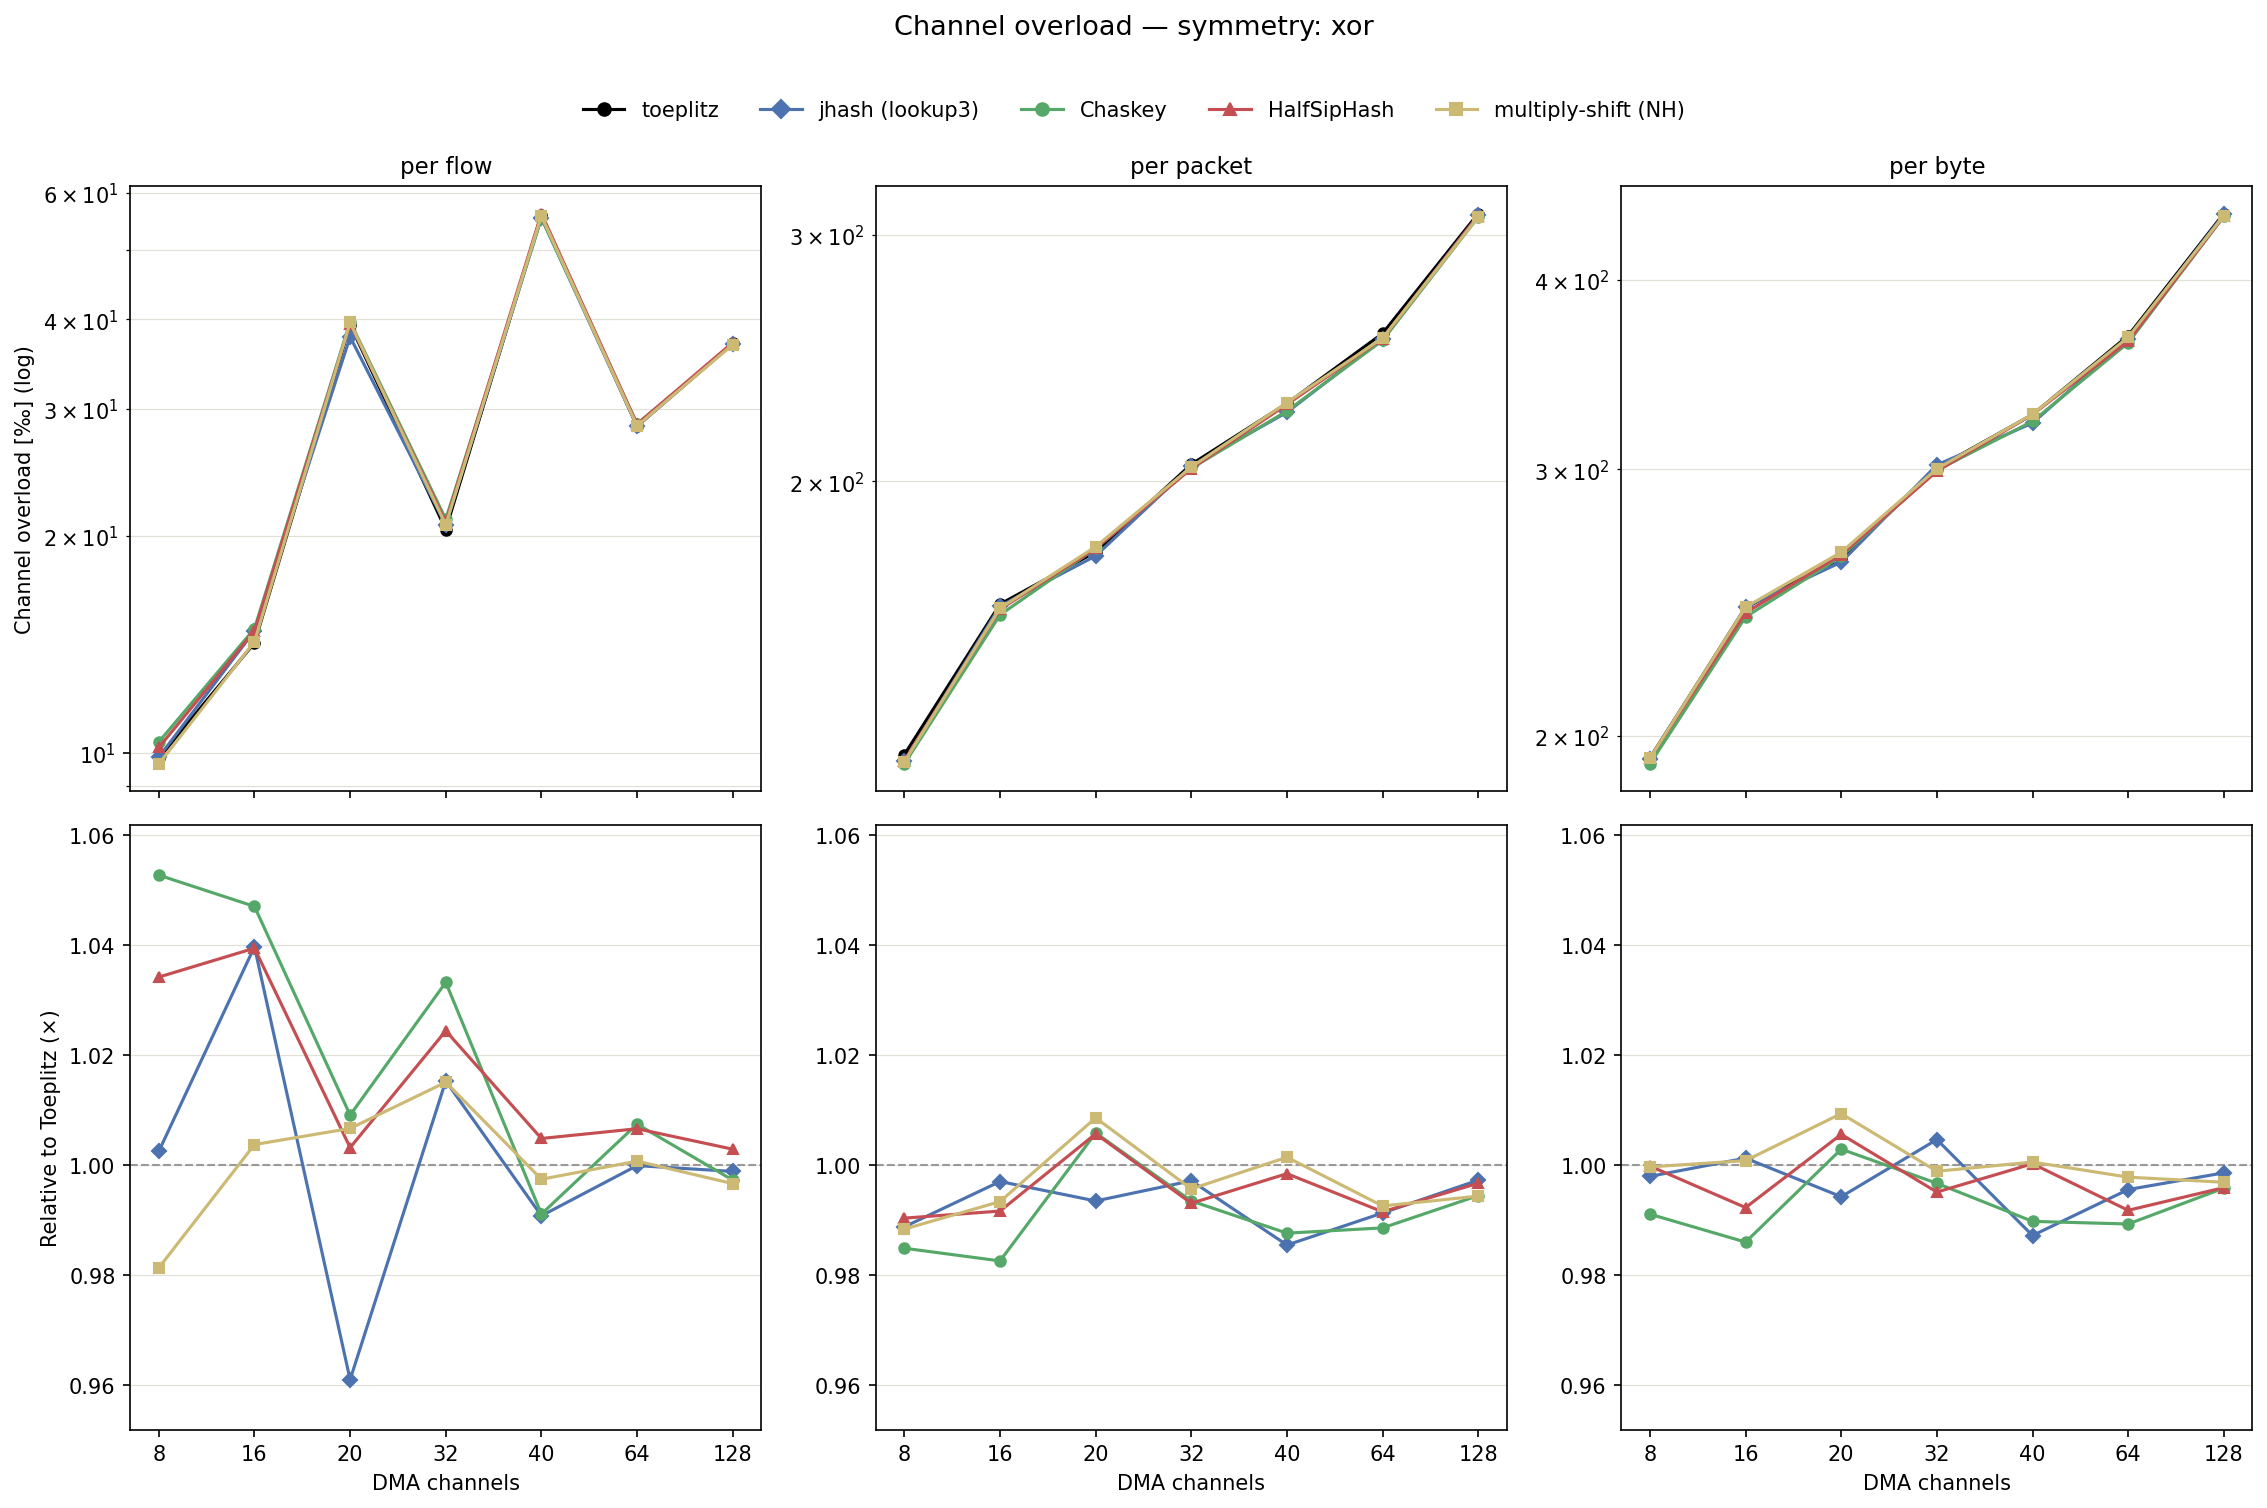
\includegraphics[width=\textwidth]{ostatne_vzorky/odid6_full_tuple/overload_xorfold.png}
    \caption{symetria XOR}
  \end{subfigure}

  \begin{subfigure}{0.60\textwidth}
    \centering
    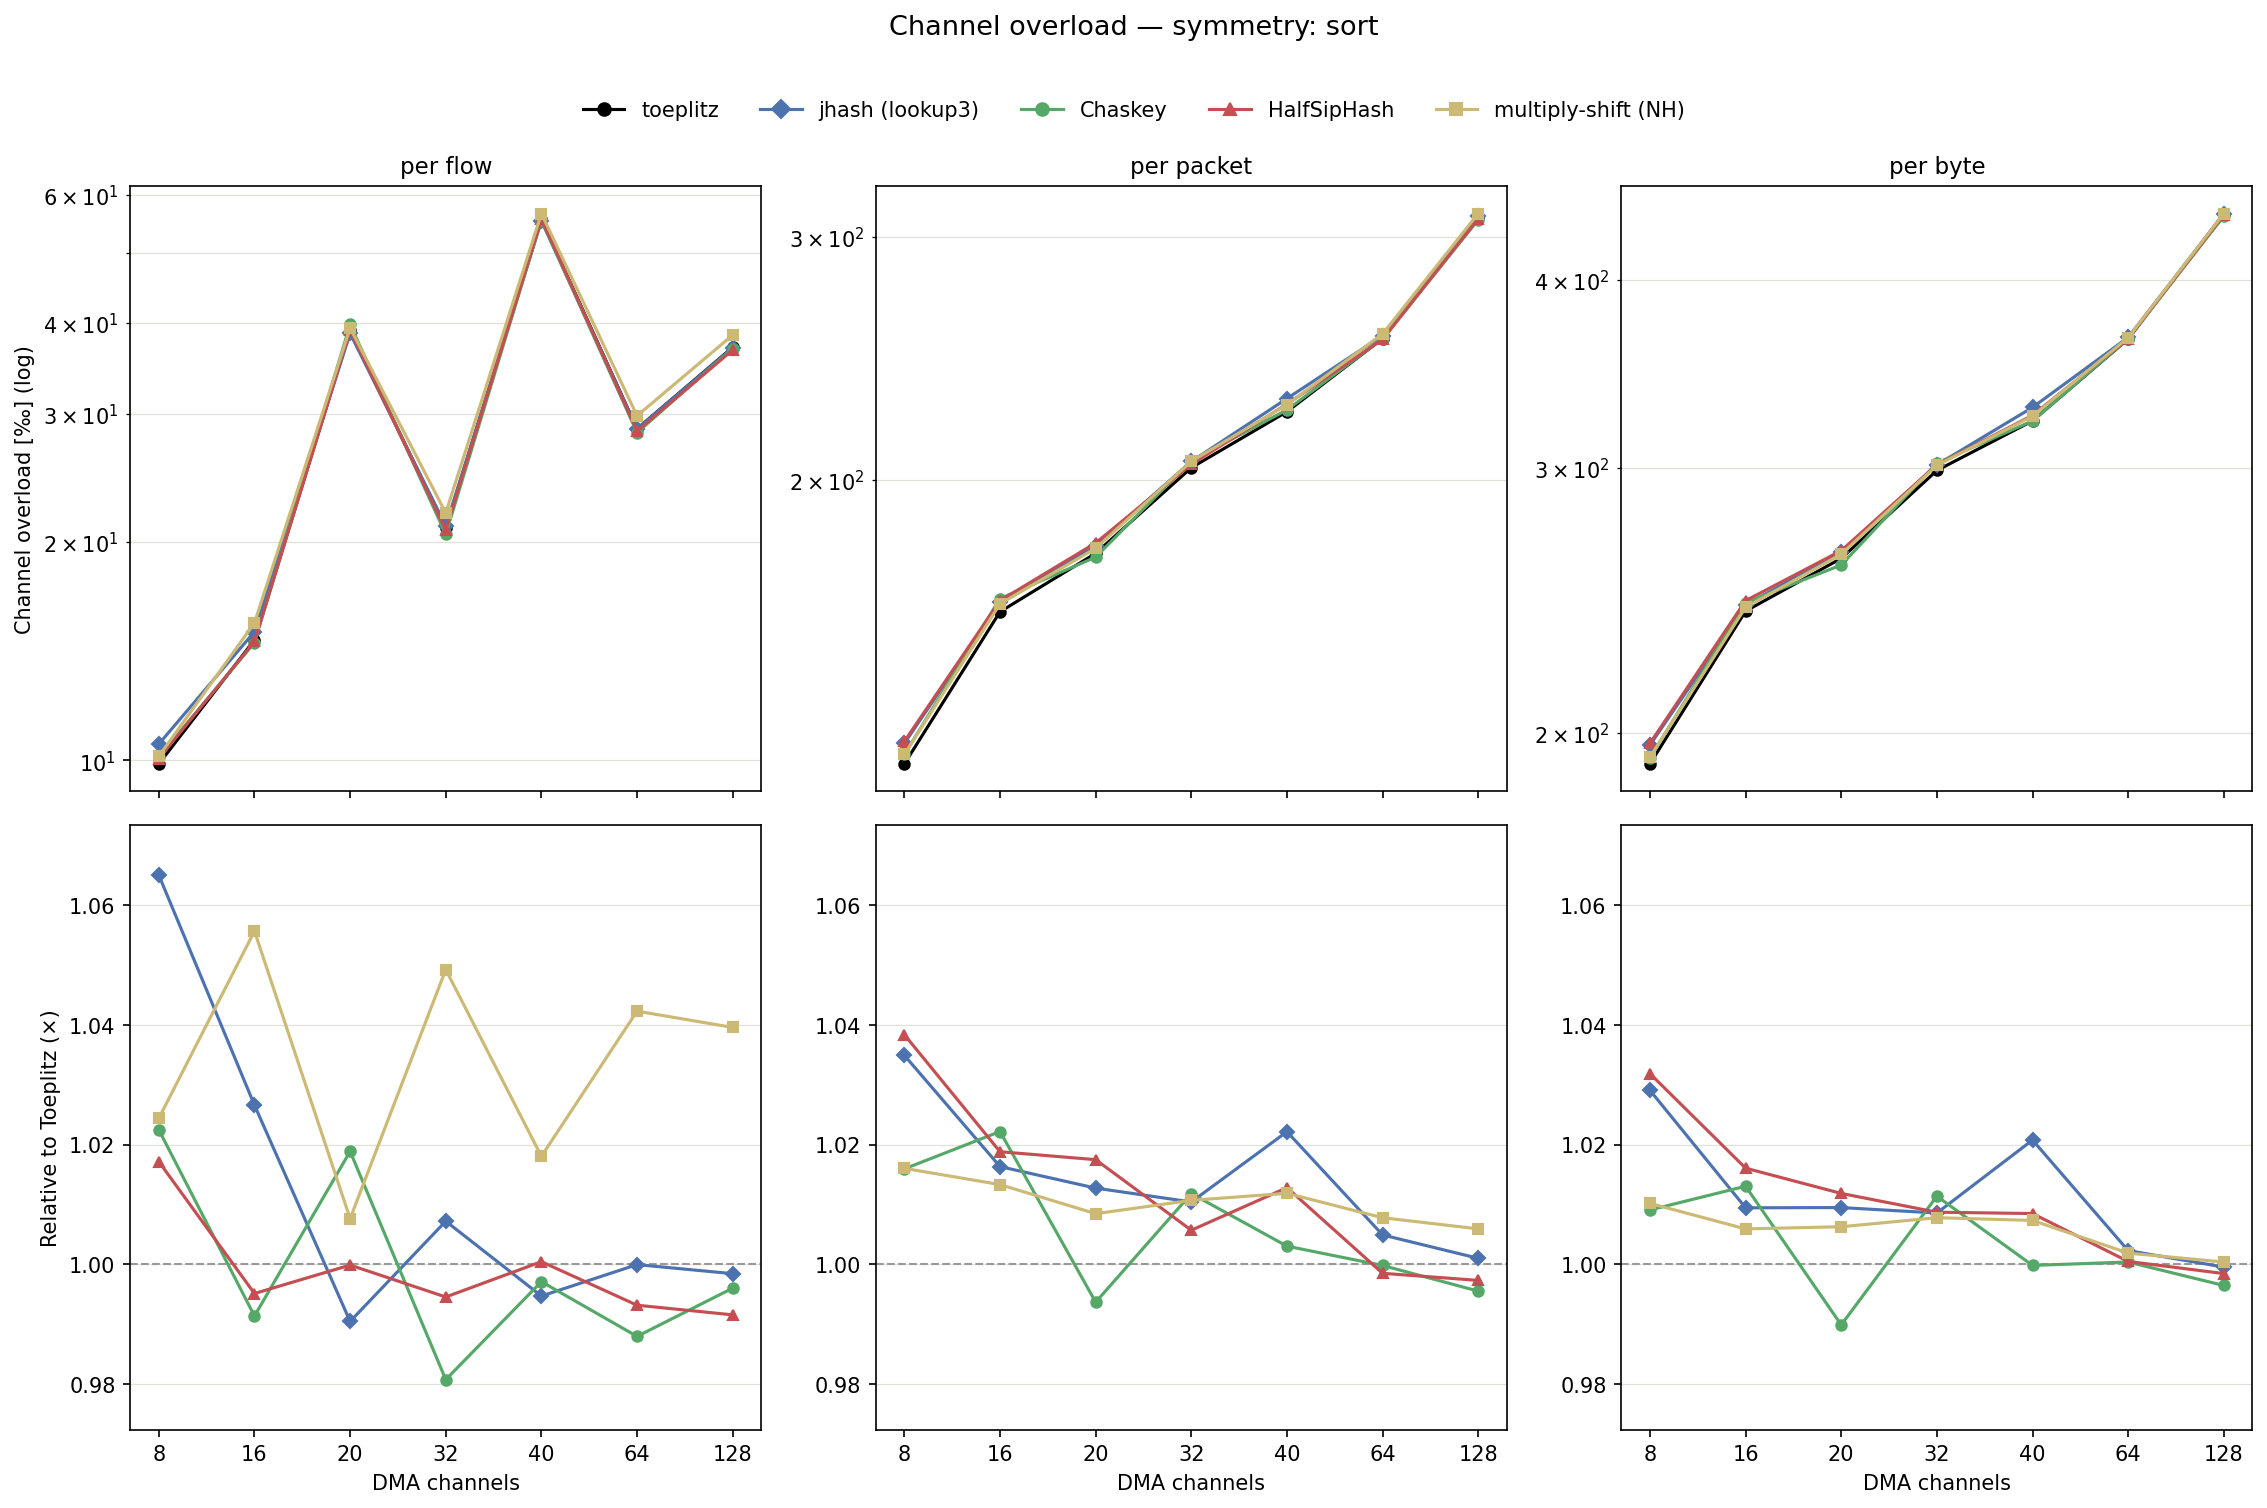
\includegraphics[width=\textwidth]{ostatne_vzorky/odid6_full_tuple/overload_sortfold.png}
    \caption{symetria sort}
  \end{subfigure}

  \caption{Preťaženie funkcií a pomer k~Toeplitzu: \texttt{odid6}, plný tuple.}
  \label{fig:b-odid6-full-tuple-overload}
\end{figure}

\begin{figure}[p]
  \centering
  \begin{subfigure}{0.54\textwidth}
    \centering
    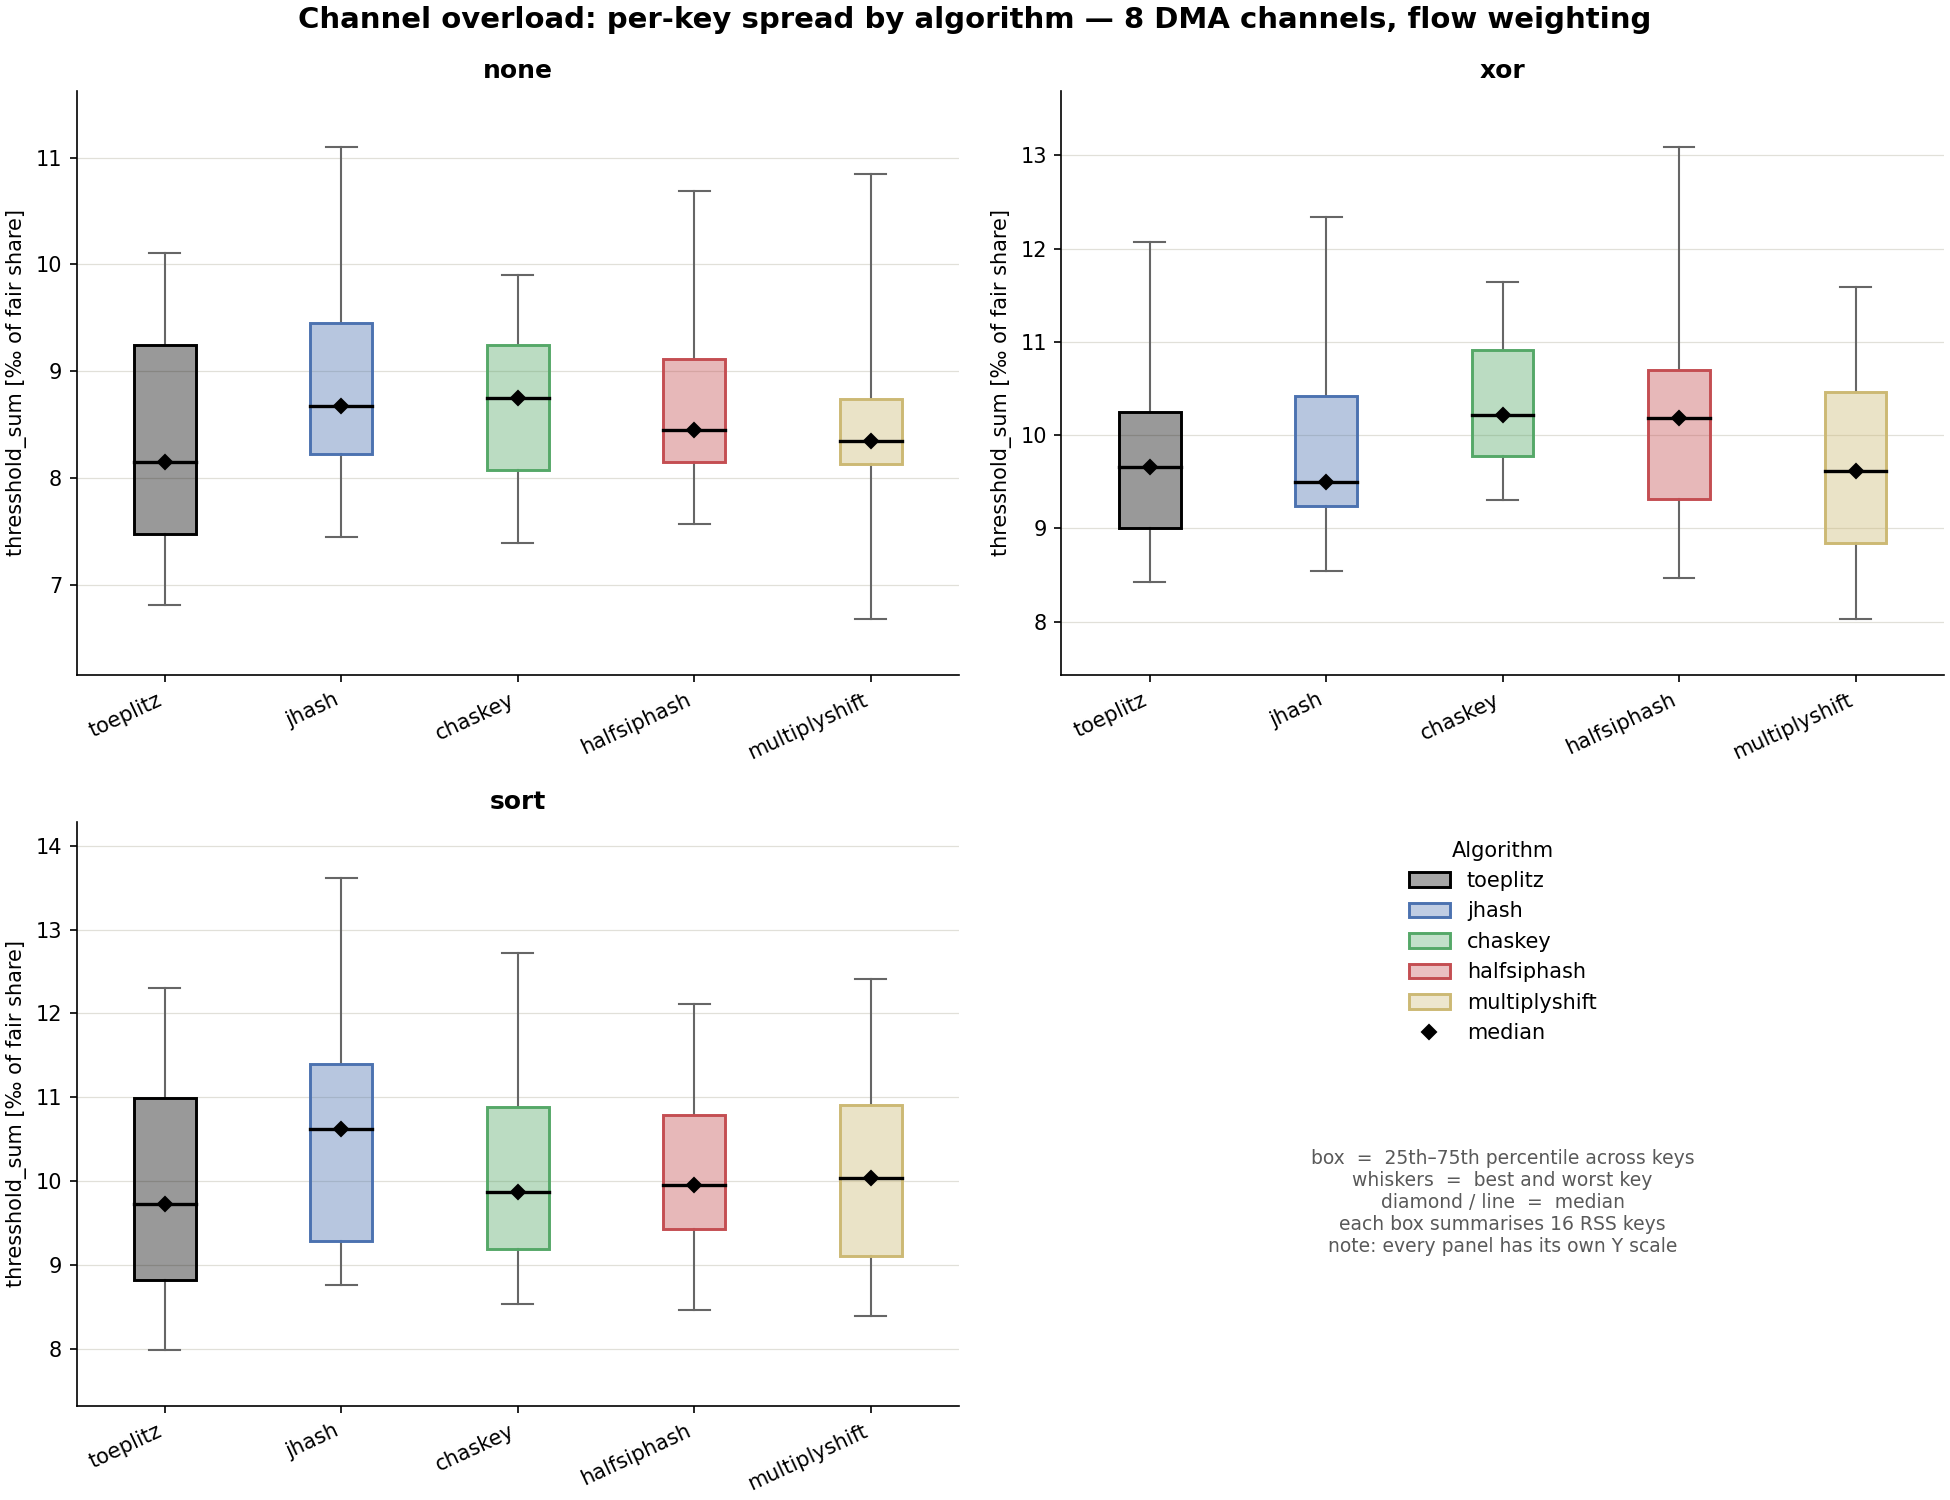
\includegraphics[width=\textwidth]{ostatne_vzorky/odid6_full_tuple/keys_8.png}
    \caption{8 kanálov}
  \end{subfigure}

  \begin{subfigure}{0.54\textwidth}
    \centering
    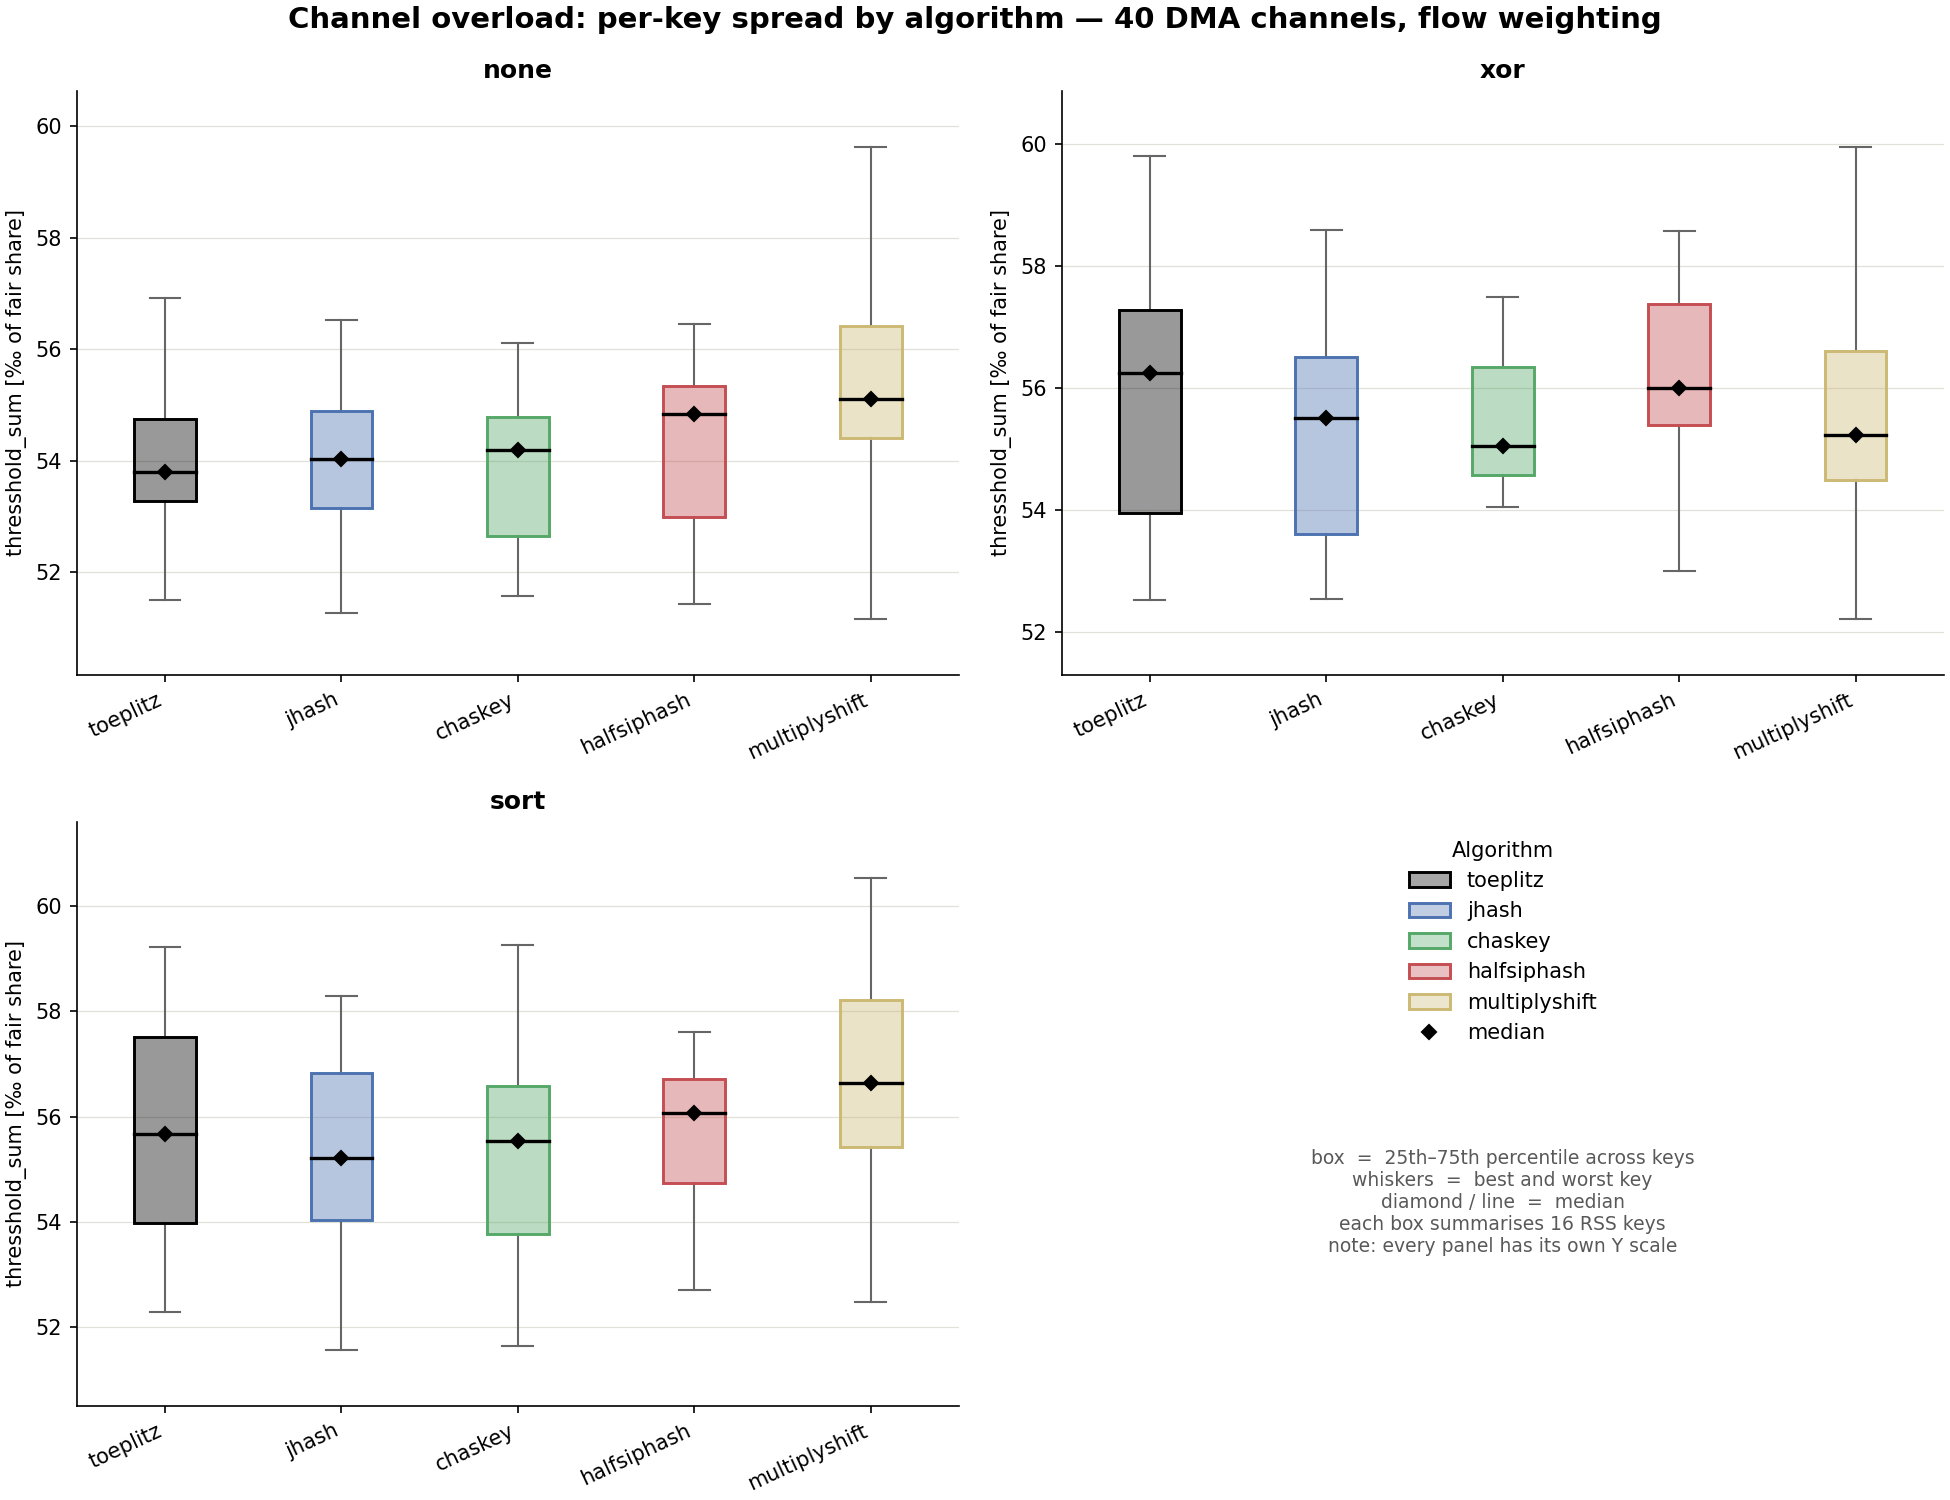
\includegraphics[width=\textwidth]{ostatne_vzorky/odid6_full_tuple/keys_40.png}
    \caption{40 kanálov}
  \end{subfigure}

  \begin{subfigure}{0.54\textwidth}
    \centering
    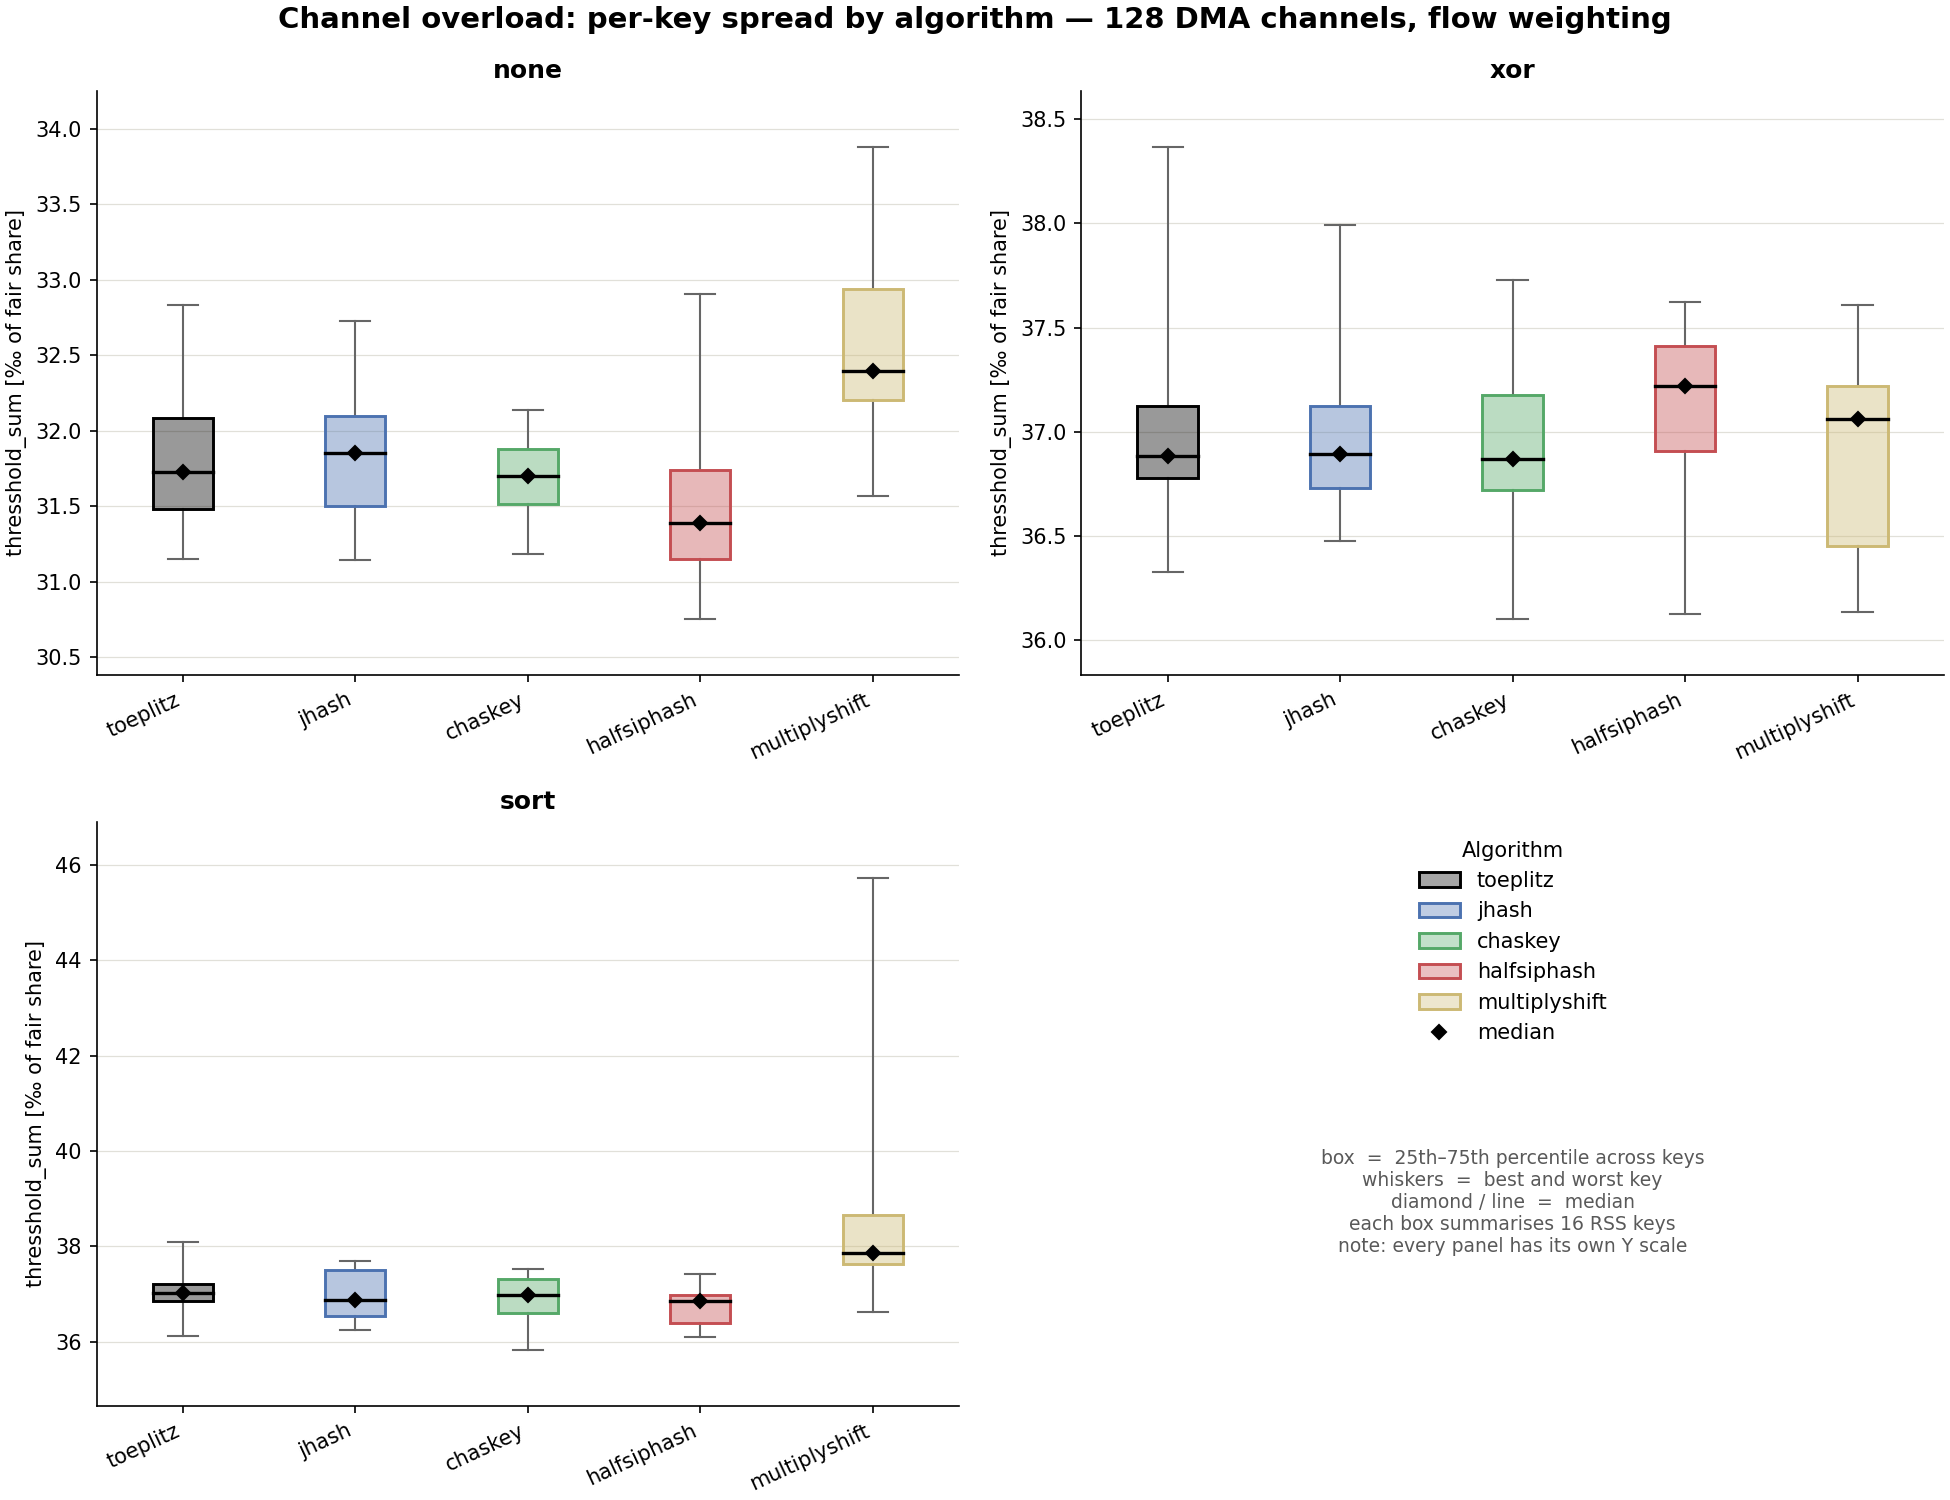
\includegraphics[width=\textwidth]{ostatne_vzorky/odid6_full_tuple/keys_128.png}
    \caption{128 kanálov}
  \end{subfigure}

  \caption{Rozptyl preťaženia medzi 16 kľúčmi pri váhe \texttt{flow}: \texttt{odid6}, plný tuple.}
  \label{fig:b-odid6-full-tuple-keys}
\end{figure}

\begin{figure}[ht]
  \centering
  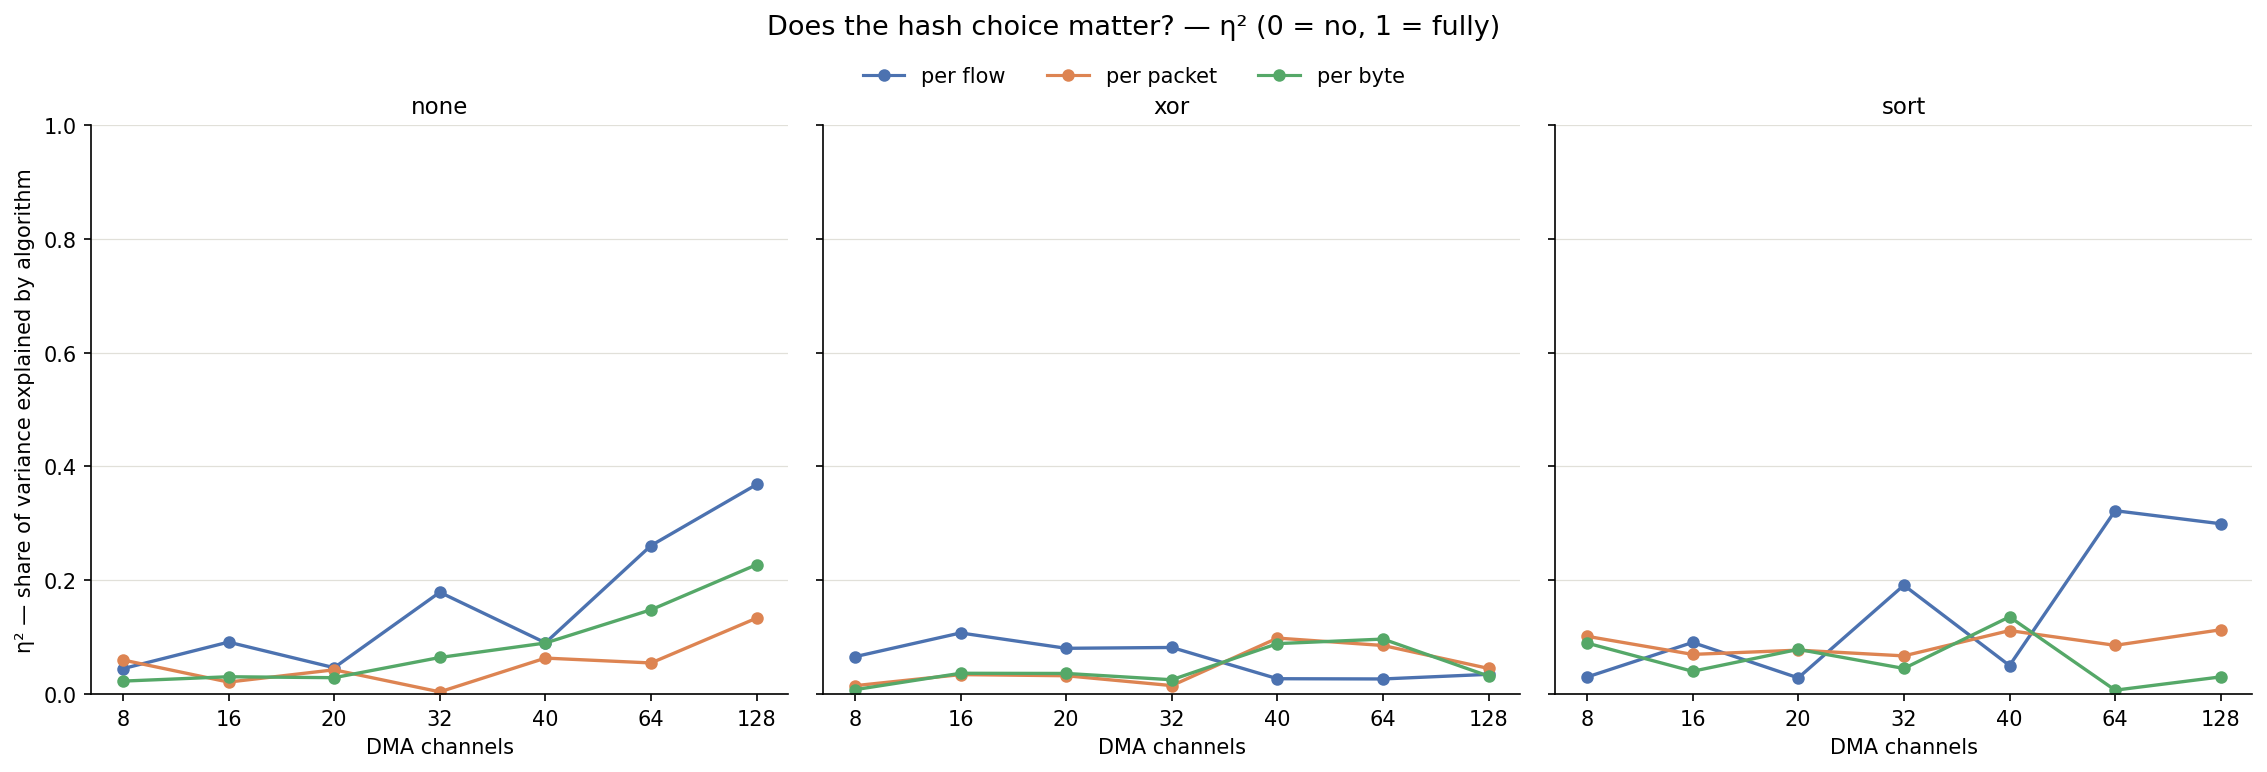
\includegraphics[width=0.9\textwidth]{ostatne_vzorky/odid6_full_tuple/spread.png}
  \caption{Podiel rozptylu vysvetlený voľbou funkcie ($\eta^2$): \texttt{odid6}, plný tuple.}
  \label{fig:b-odid6-full-tuple-spread}
\end{figure}

\clearpage
\begin{figure}[p]
  \centering
  \begin{subfigure}{0.60\textwidth}
    \centering
    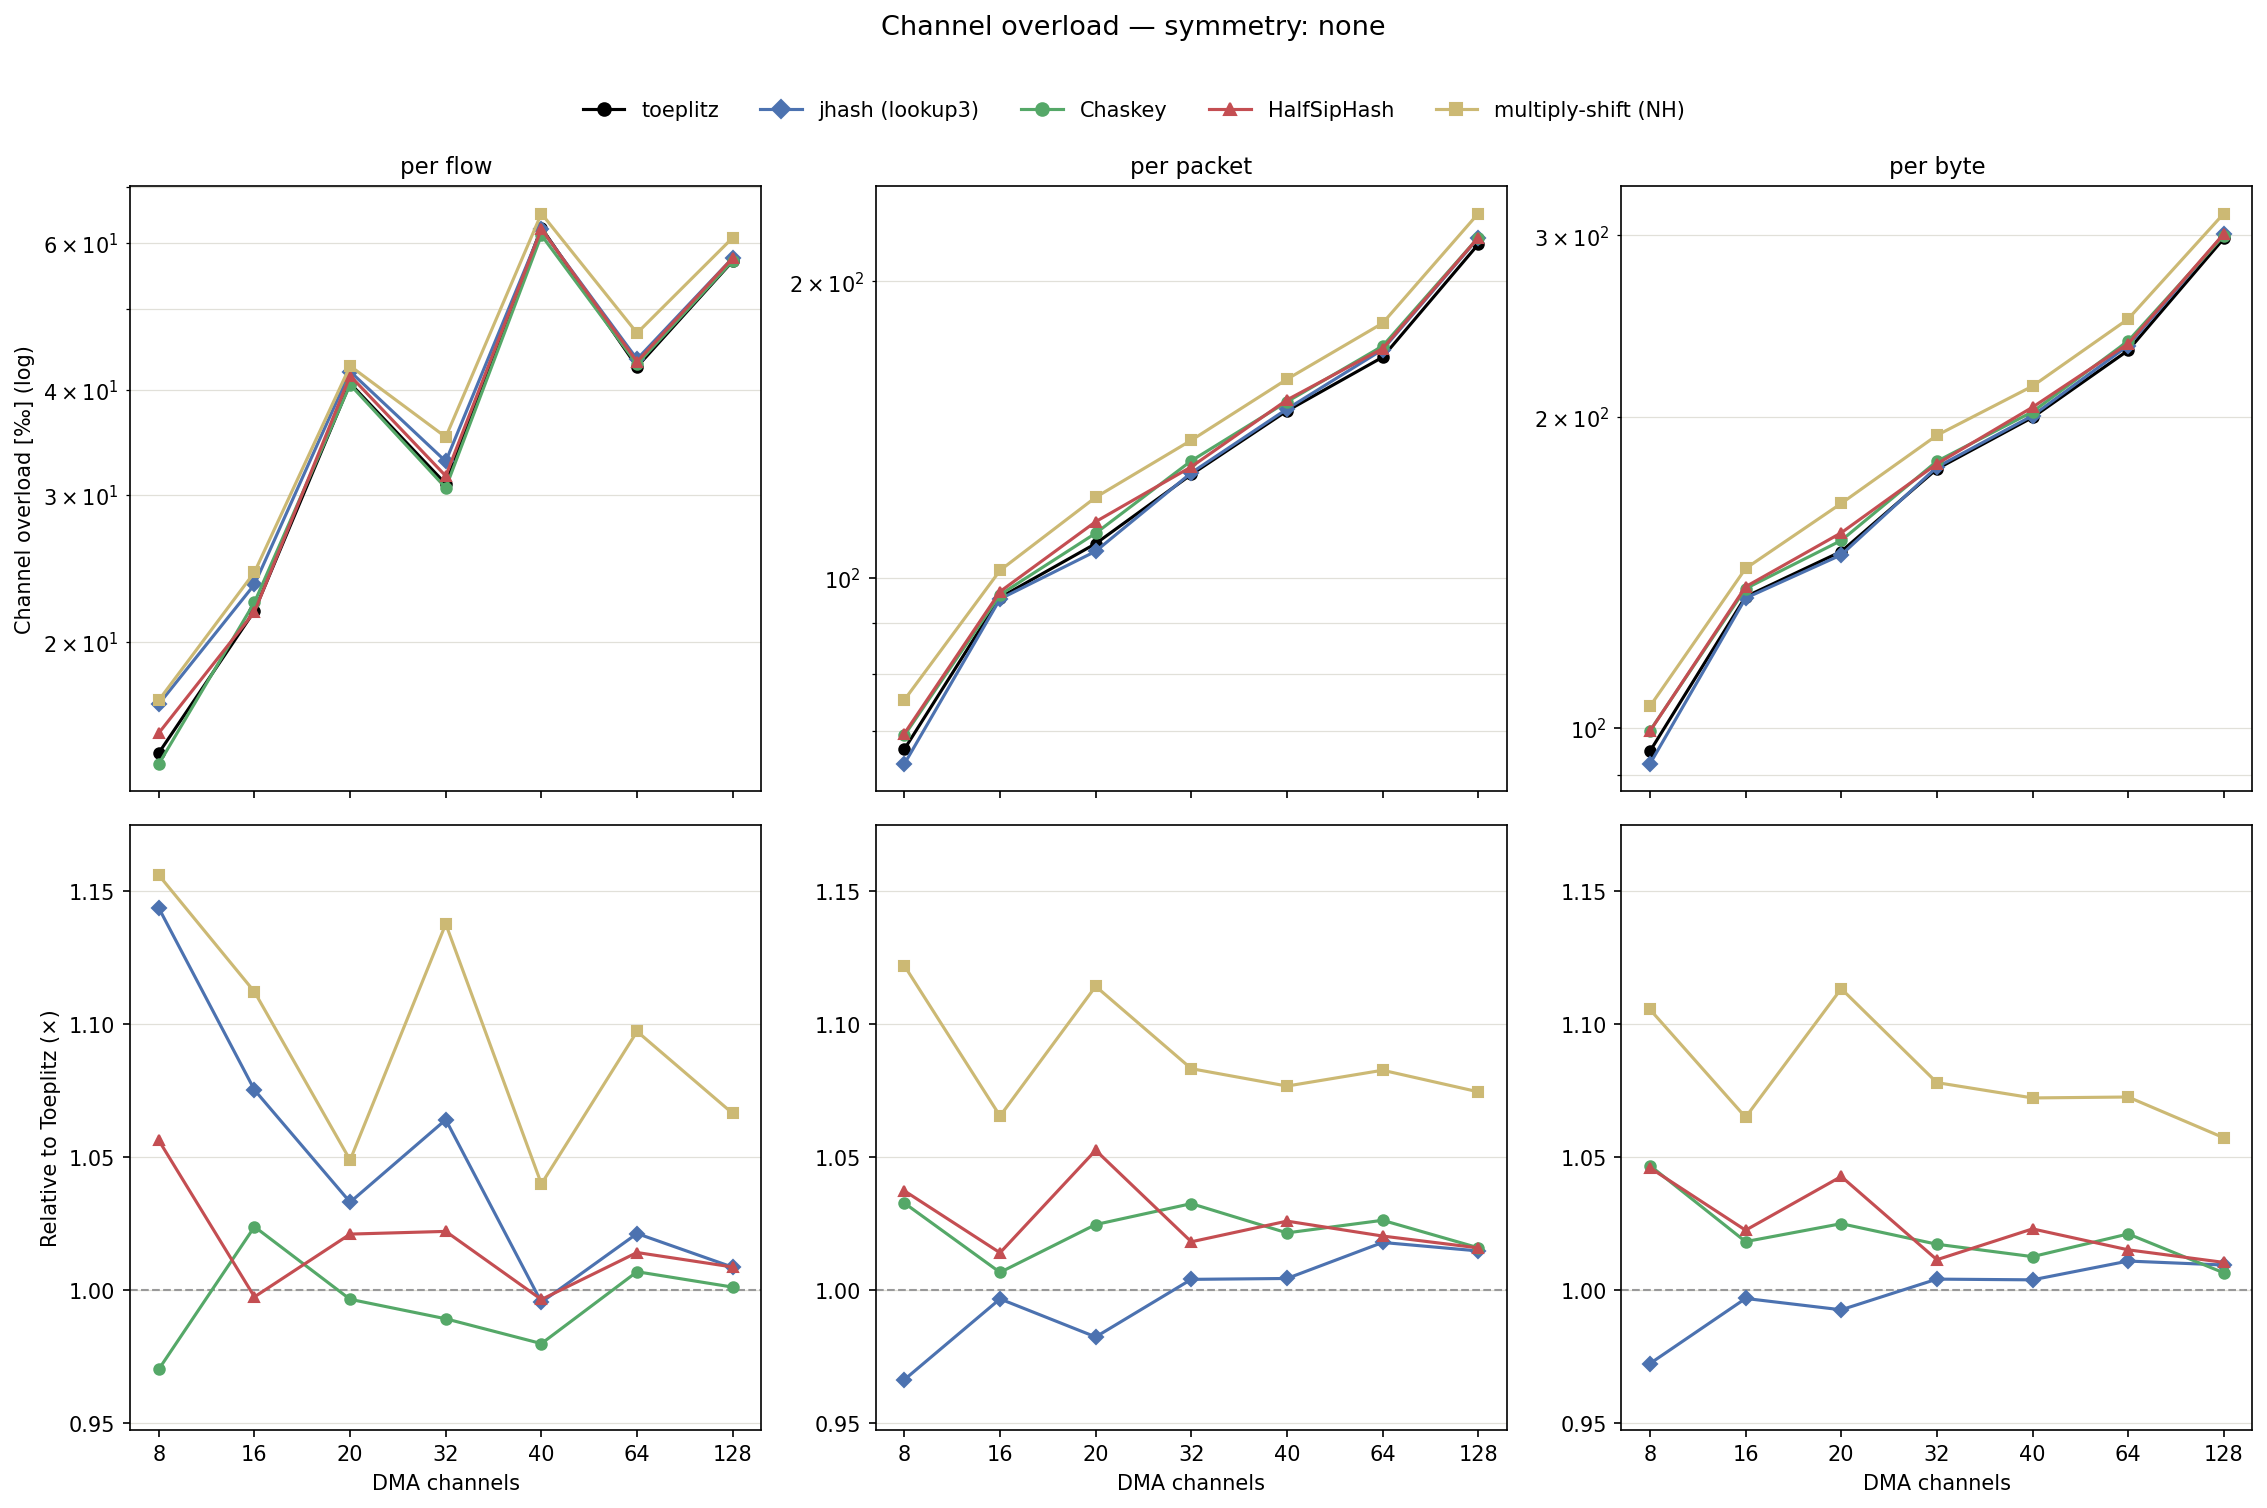
\includegraphics[width=\textwidth]{ostatne_vzorky/odid1_ip_only/overload_none.png}
    \caption{bez symetrie}
  \end{subfigure}

  \begin{subfigure}{0.60\textwidth}
    \centering
    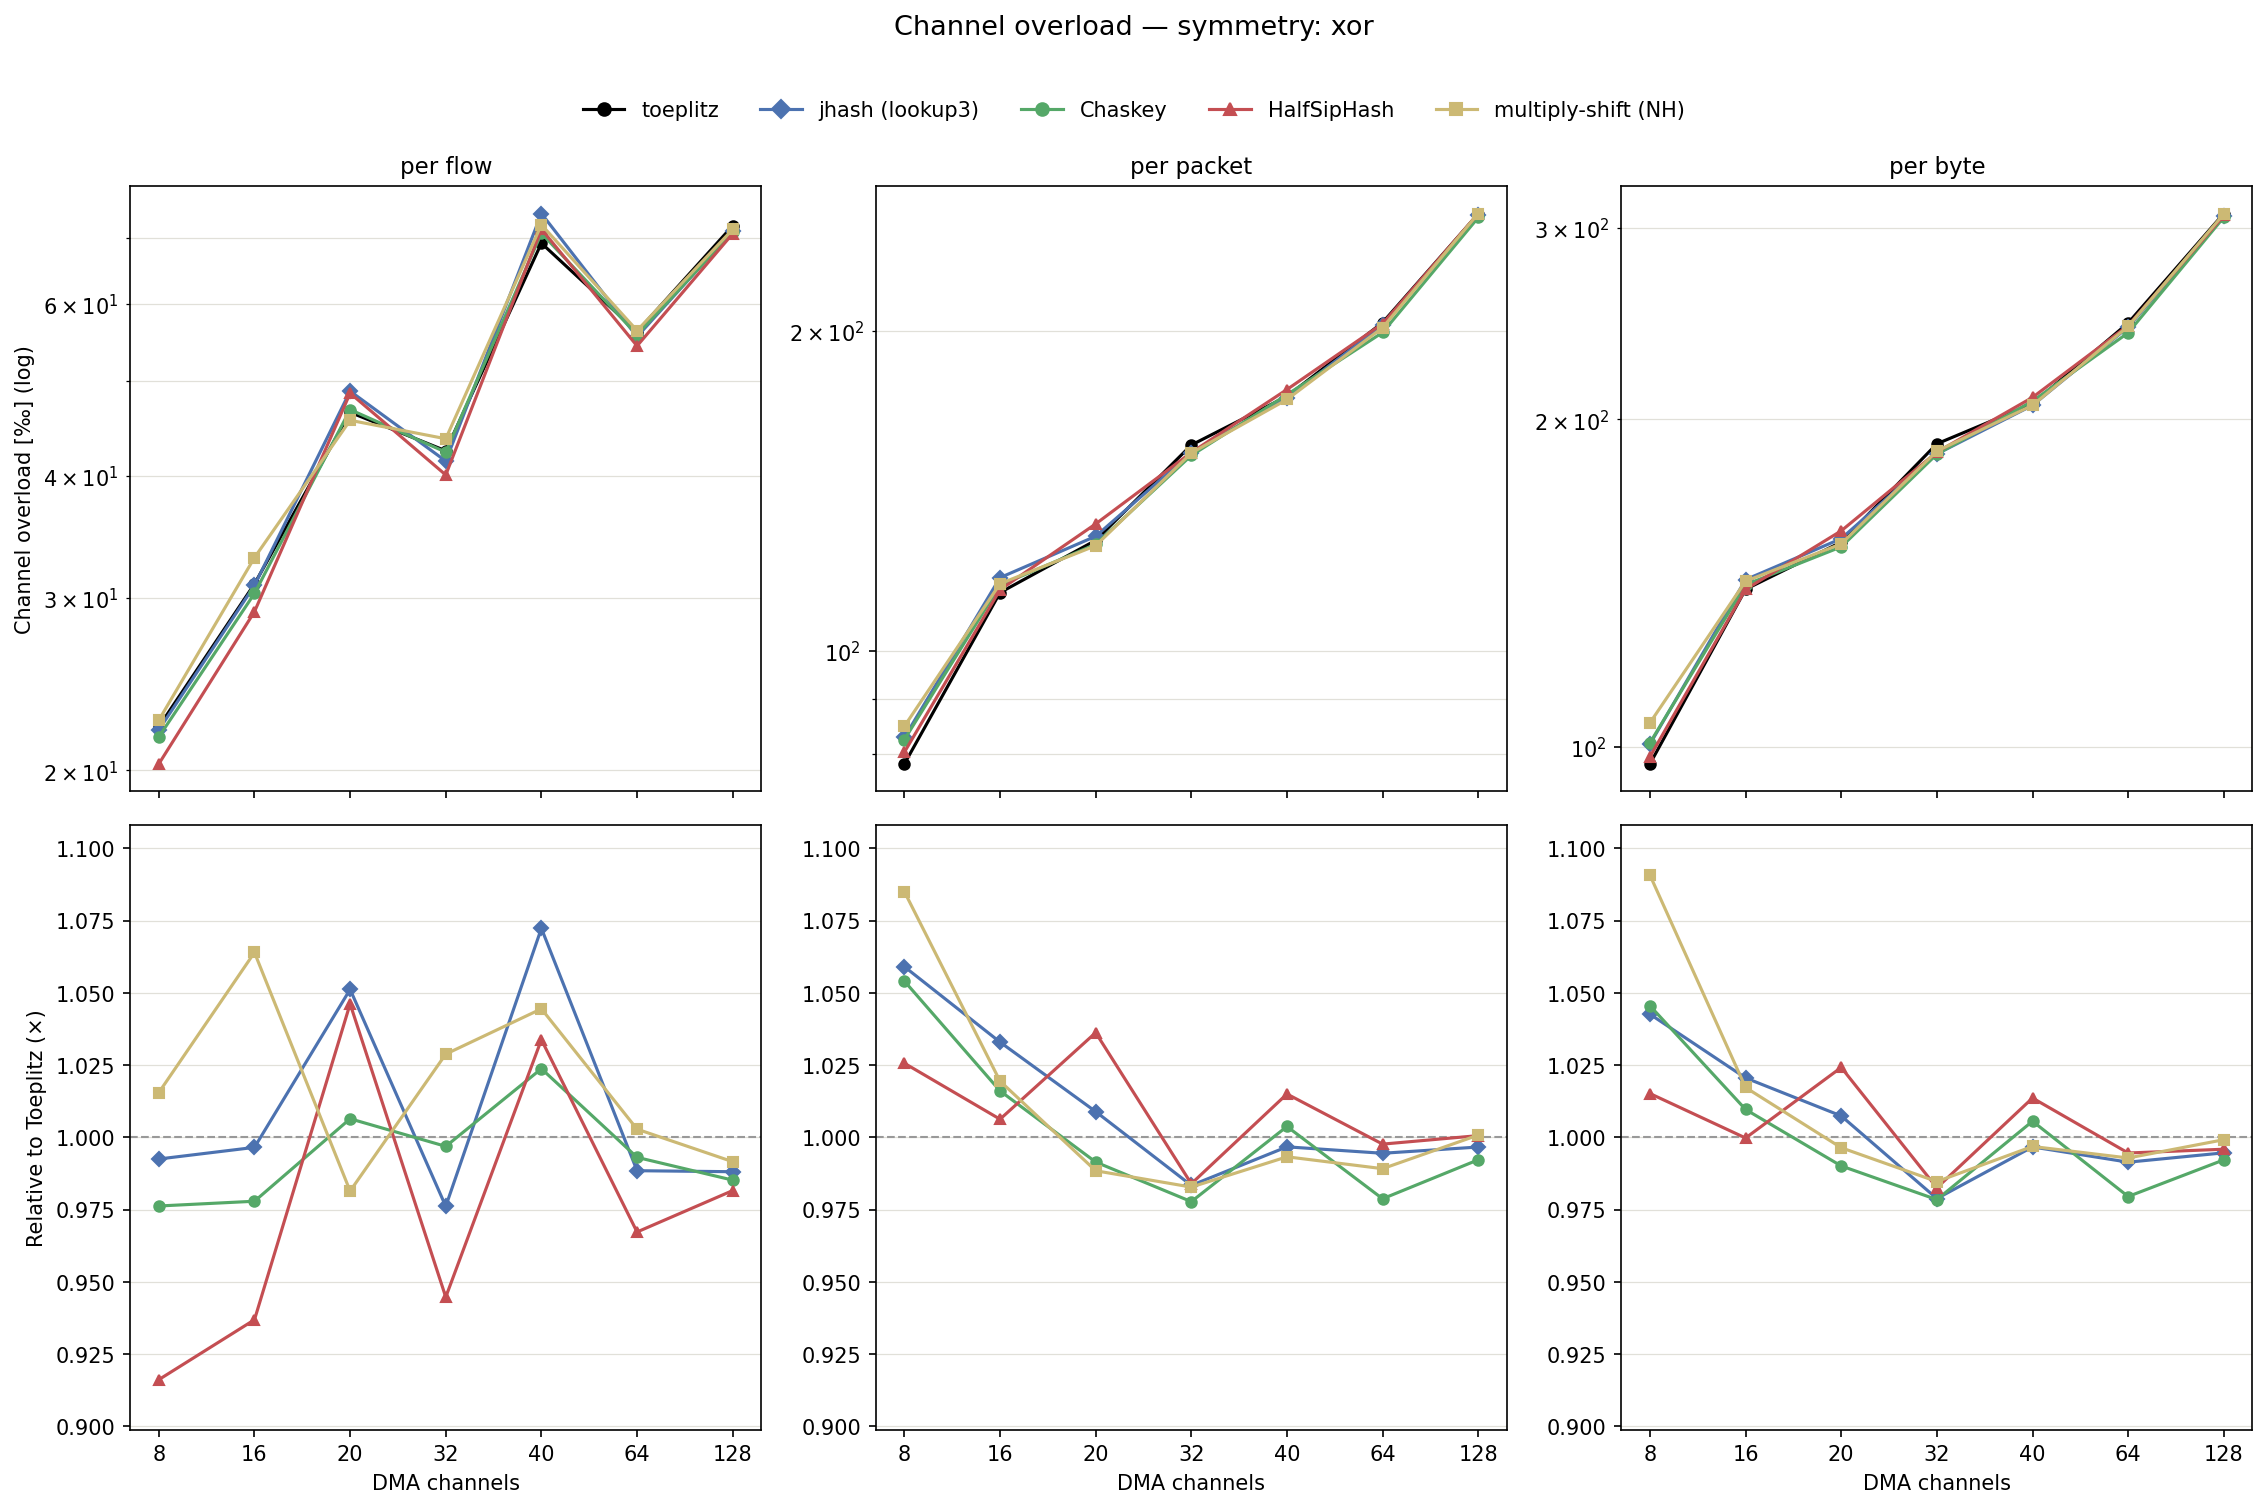
\includegraphics[width=\textwidth]{ostatne_vzorky/odid1_ip_only/overload_xorfold.png}
    \caption{symetria XOR}
  \end{subfigure}

  \begin{subfigure}{0.60\textwidth}
    \centering
    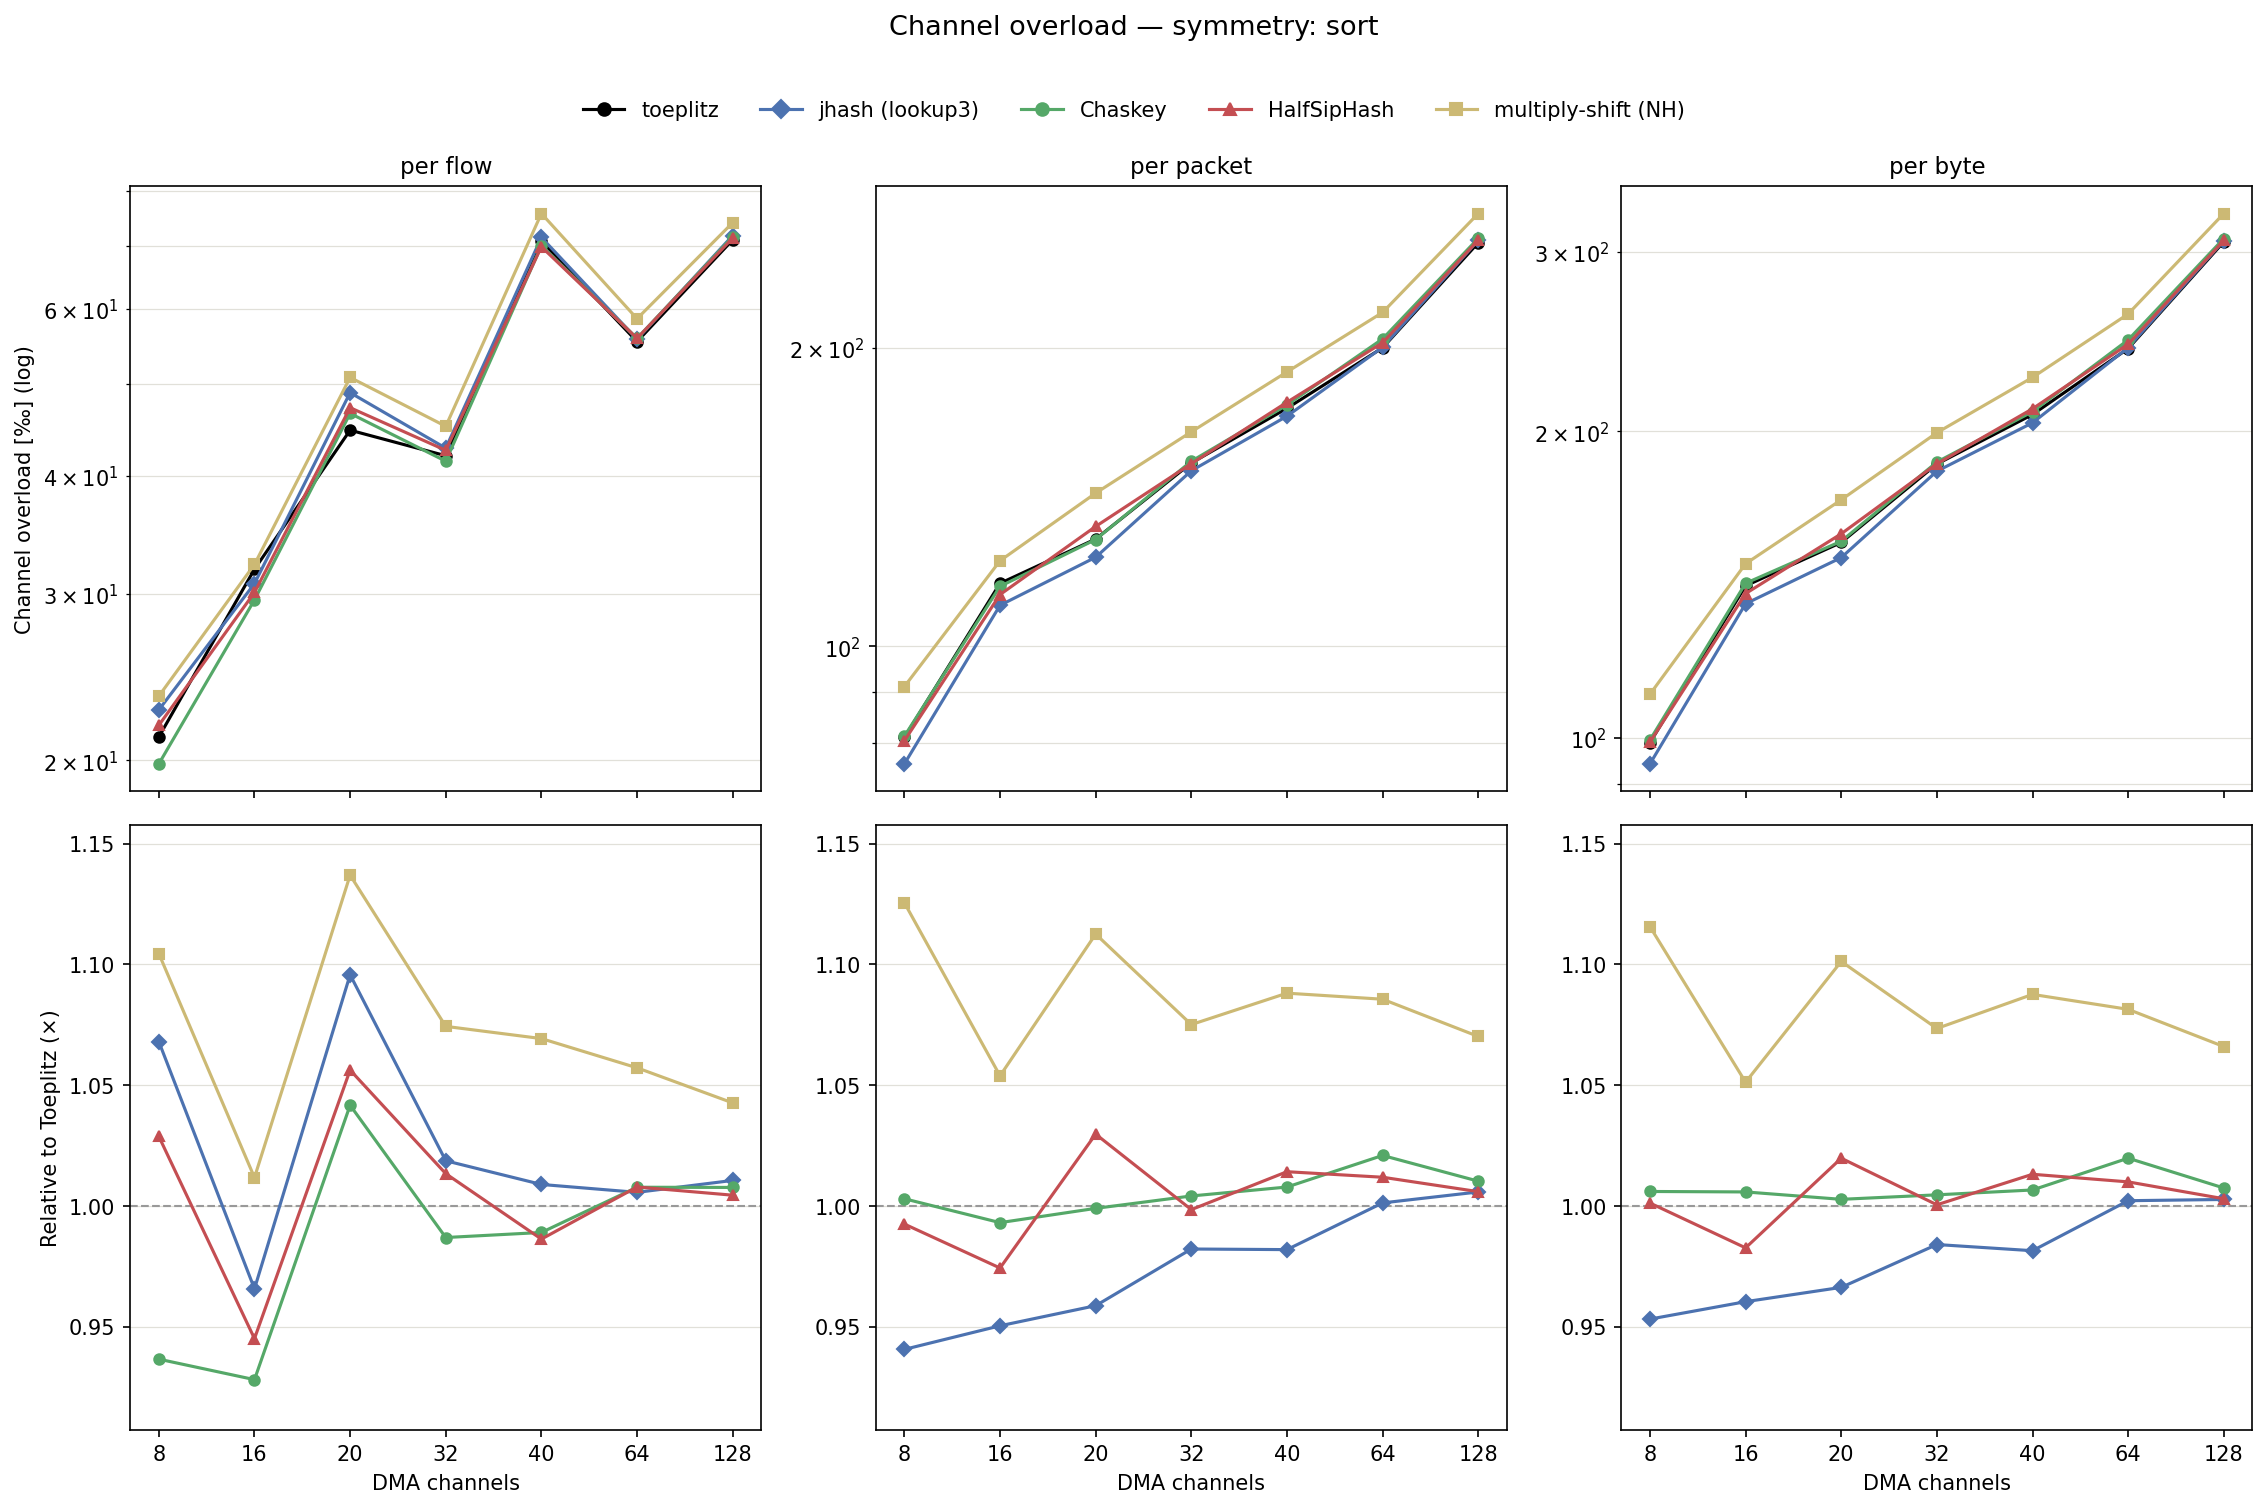
\includegraphics[width=\textwidth]{ostatne_vzorky/odid1_ip_only/overload_sortfold.png}
    \caption{symetria sort}
  \end{subfigure}

  \caption{Preťaženie funkcií a pomer k~Toeplitzu: \texttt{odid1}, iba IP adresy.}
  \label{fig:b-odid1-ip-only-overload}
\end{figure}

\begin{figure}[p]
  \centering
  \begin{subfigure}{0.54\textwidth}
    \centering
    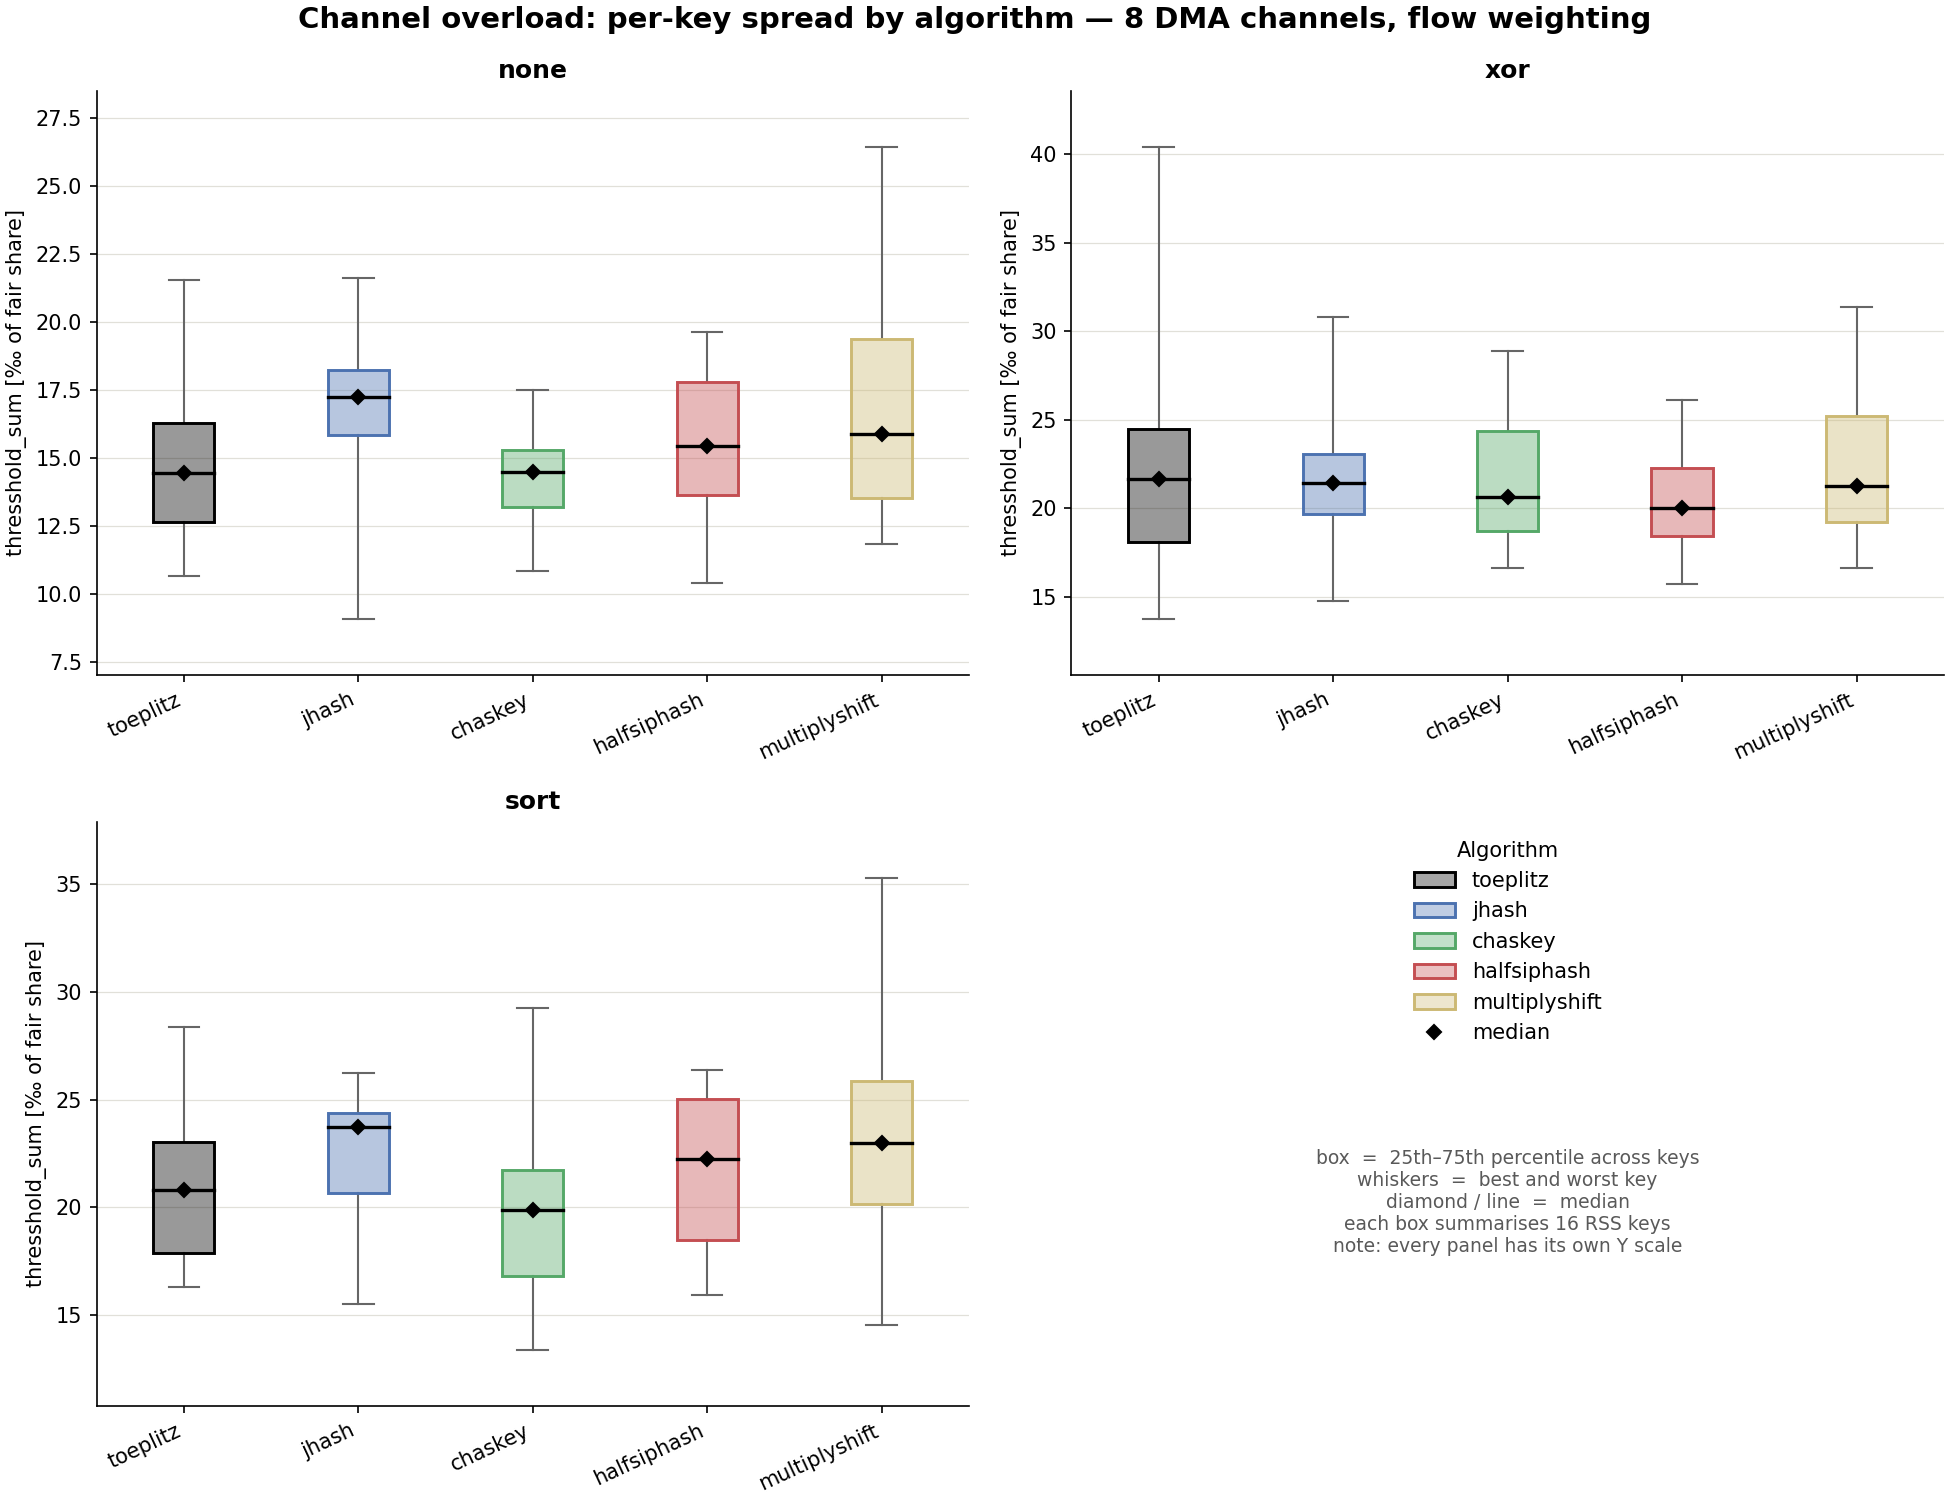
\includegraphics[width=\textwidth]{ostatne_vzorky/odid1_ip_only/keys_8.png}
    \caption{8 kanálov}
  \end{subfigure}

  \begin{subfigure}{0.54\textwidth}
    \centering
    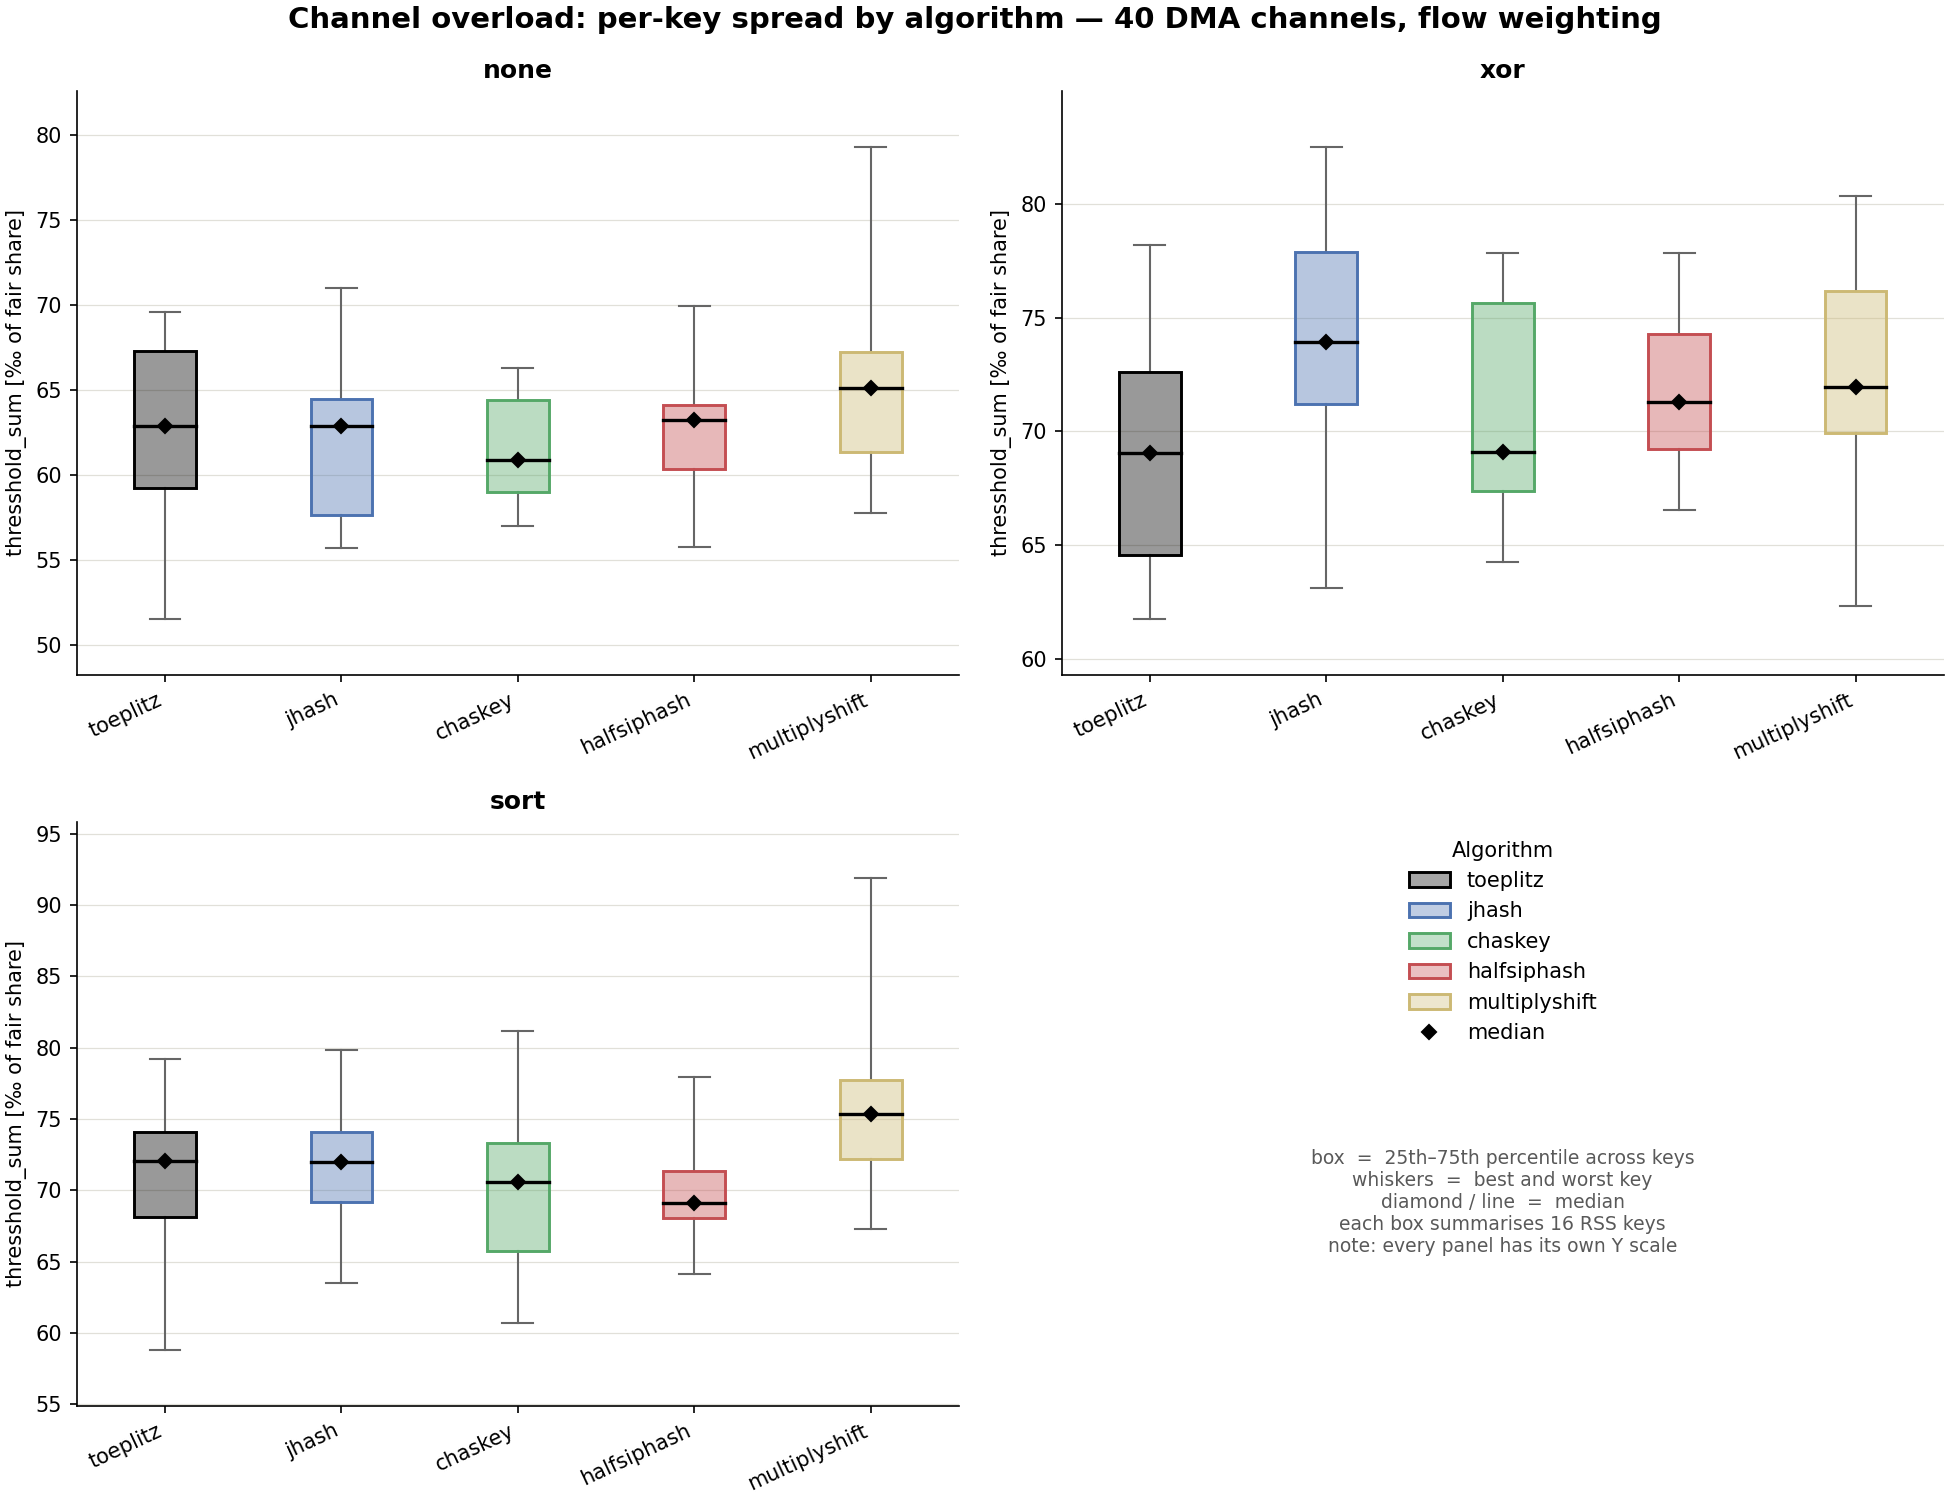
\includegraphics[width=\textwidth]{ostatne_vzorky/odid1_ip_only/keys_40.png}
    \caption{40 kanálov}
  \end{subfigure}

  \begin{subfigure}{0.54\textwidth}
    \centering
    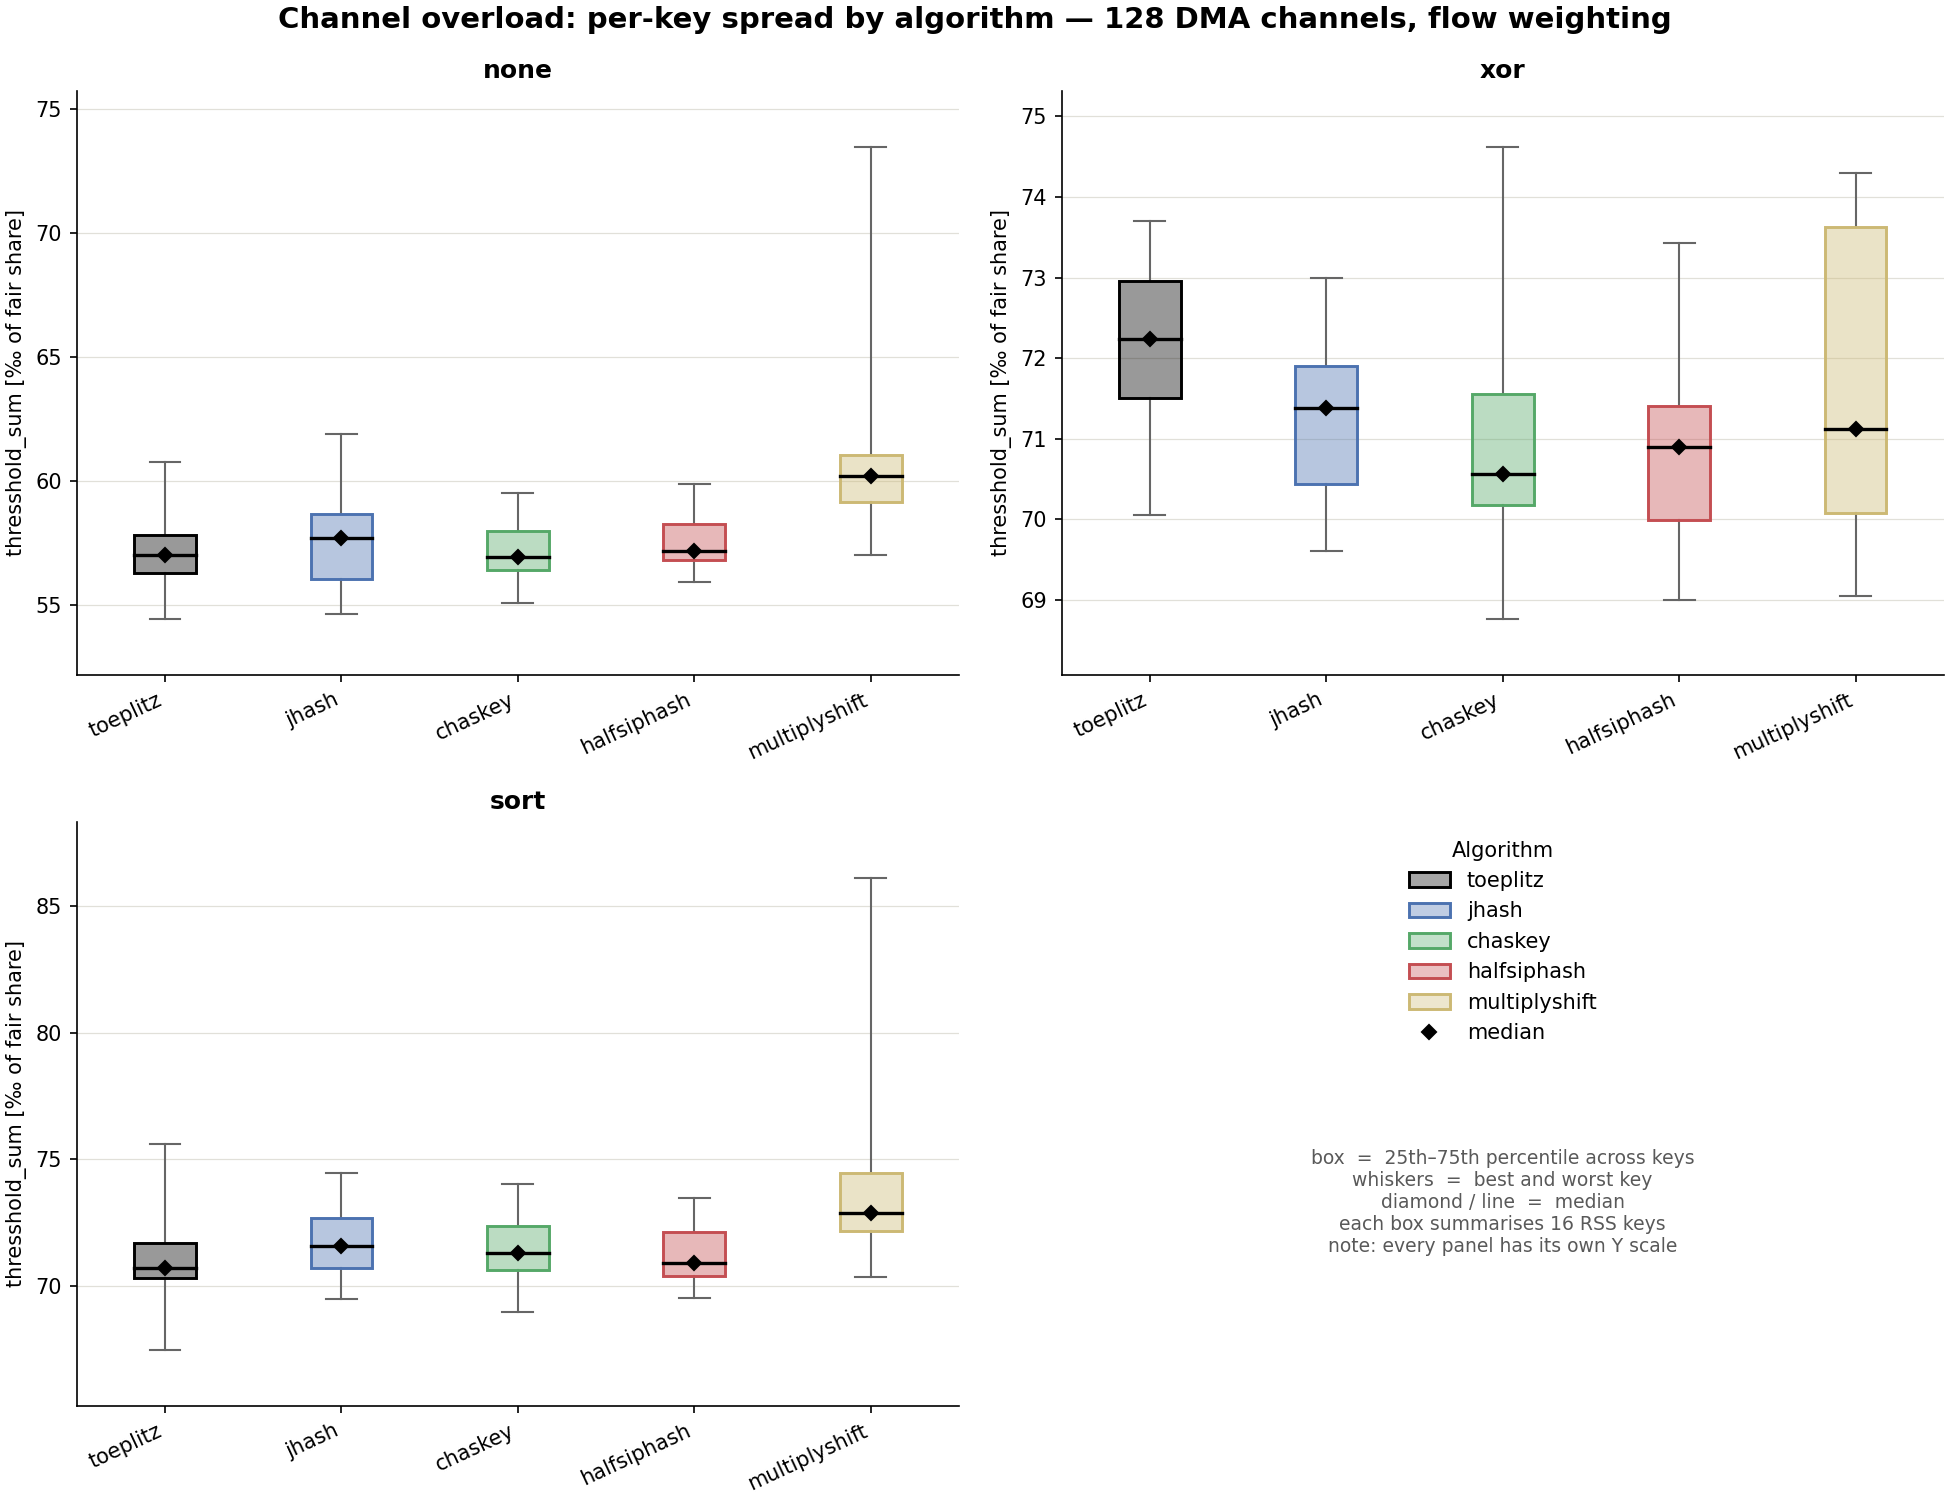
\includegraphics[width=\textwidth]{ostatne_vzorky/odid1_ip_only/keys_128.png}
    \caption{128 kanálov}
  \end{subfigure}

  \caption{Rozptyl preťaženia medzi 16 kľúčmi pri váhe \texttt{flow}: \texttt{odid1}, iba IP adresy.}
  \label{fig:b-odid1-ip-only-keys}
\end{figure}

\begin{figure}[ht]
  \centering
  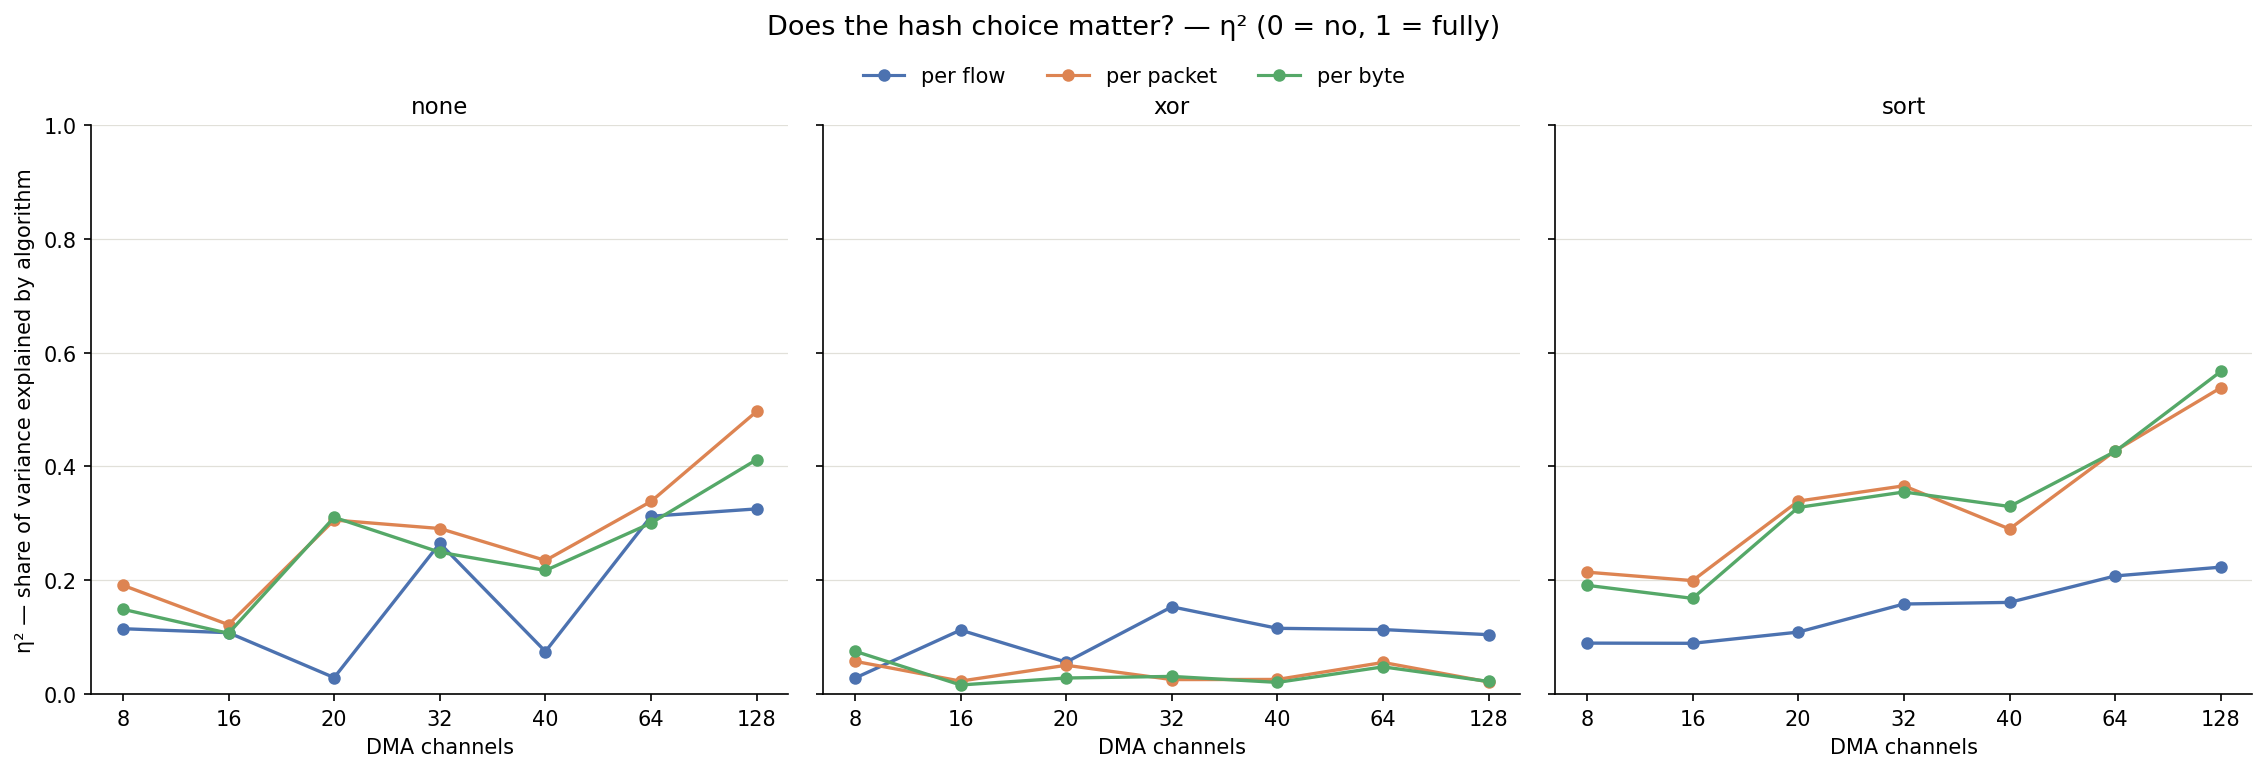
\includegraphics[width=0.9\textwidth]{ostatne_vzorky/odid1_ip_only/spread.png}
  \caption{Podiel rozptylu vysvetlený voľbou funkcie ($\eta^2$): \texttt{odid1}, iba IP adresy.}
  \label{fig:b-odid1-ip-only-spread}
\end{figure}

  % !TEX root = ../projekt.tex
% =============================================================================
% STAV: hotové podľa aktuálneho kódu.
% =============================================================================
\chapter{Návod na spustenie simulátora}
\label{app:manual}

\section*{Preklad a spustenie}
\begin{lstlisting}
make                      # build rss_sim
./run.sh                  # simulation + table + plot, uses config.conf
./run.sh my_test.conf     # the same with another config
./rss_sim config.conf     # simulation only
\end{lstlisting}

\section*{Výstup}
Výsledkom je súbor CSV podľa kľúča \texttt{out} a graf s~rovnakým menom a príponou \texttt{.png}.
\begin{lstlisting}
method,window,num_channels,overload,fairness,chi
hash,1,8,110.914,0.922365,0.0851074
\end{lstlisting}
Riadky \texttt{hash} sú priemerom cez všetky kľúče. Orákulum \texttt{jsq} kľúče nepoužíva.

\TODO{Doplniť závislosti (kompilátor C++17, Python, pandas, matplotlib) a popis všetkých kľúčov.}


\end{document}
